% !TeX root = ../../book.tex
\chapter[函数与基数]{函数与基数:输入、输出和集合的大小}

% !TeX root = ../../../book.tex

\section{引言}

我们将继续探讨函数的第二个章节。在本章中,我们将正式\emph{定义}函数。具体来说,函数实际上是一种具有特定性质的\textbf{关系}。这也是我们之前花时间研究关系的原因 --- 除了关系本身的趣味性和实用性之外。定义函数后,我们将通过大量实例和证明来研究函数可能具有的各种特性。在这个过程中,我们将用到之前所有学过的概念,特别是 \ref{sec:section4.9} 节中的证明技巧。

在本章的后半部分,我们将介绍\emph{双射}函数 (Bijective Function) 的概念,即两个集合元素的一一对应关系,用来讨论集合的``大小''及其比较方法。这个主题被称为\emph{基数} (Cardinality),它将揭示一些关于无限集的惊人且反直觉的事实。这也为我们进入下一章奠定基础,在下一章中,我们将集中研究有限集及其计数方法。

% !TeX root = ../../../book.tex

\subsection{目标}

以下简要说明本章在本书中的定位。我们将阐释先前内容如何发挥作用,阐述研究本章主题的动机,明确学习目标,并提示阅读时的关注重点。我们会先列出本章的核心目标及学成后应掌握的技能,后续章节将详细展开。学完本章后,请返回此处核验:你是否理解所有目标?能否阐述其重要性?能否定义相关术语?能否运用相关技术?

\textbf{学完本章后,你应该能够……}

\begin{itemize}
    \item 定义函数并给出多个示例。
    \item 借助函数的非形式化描述与可视化图示,构建关于函数性质(示例与反例)的形式化论证。
    \item 在函数框架下定义集合的像 (Image) 与原像 (Pre-image),并证明相关运算性质。
    \item 阐述函数的性质特征,运用相关方法判定并证明给定函数是否具备特定性质。
    \item 求函数复合,阐释如何构造新函数,并分析证明复合运算对函数性质的影响。
    \item 描述双射函数 (Bijective Function) 与反函数 (Inverse Function) 的关联,运用其解决问题并证明结论。
    \item 利用双射定义集合的基数 (Cardinality),并证明相关基数定理。
    \item 辨析有限集、可数无限集与不可数无限集之间的区别,并提供各类集合的典型实例。
\end{itemize}

% !TeX root = ../../../book.tex

\subsection{承上}

前一章介绍的重要概念\textbf{关系}将在本章发挥重要作用。我们已经提到,\textbf{函数}实际上是关系的一种特例,这一点将在我们对函数的正式定义中体现。

至于前一章讨论的其他概念,比如等价关系和数论结果,它们在本章中不会直接出现。也就是说,本章中我们探讨的函数及其性质,并不依赖于这些概念。然而,我们会利用这些概念来设计一些有趣的示例和练习。

% !TeX root = ../../../book.tex

\subsection{启下}

正如我们在上一章提到的,你很可能已经对函数的概念和使用方法有了一些直观的理解。这些理解可能来自你之前的数学课程,或者来自计算机编程的经验。我们一直强调,希望能正确、正式地用\emph{数学方式}定义我们所研究的概念,函数也不例外!通过正式定义,我们可以更好地讨论一些你可能以前见过但无法清楚表达的函数性质。此外,函数的某些特定性质还会帮助我们讨论集合的\emph{基数}。请相信我,如果不先探讨函数,我们就无法对这个主题进行深入讨论。


% !TeX root = ../../../book.tex

\subsection{忠告}

我们还要重申上一章中的一些忠告和建议。我们正在继续探索一些抽象的数学领域。本章特别是要将一个你可能在视觉和直觉上熟悉的概念放在更严格的基础之上。我们会尽可能利用大家的直觉,但也无法避免地需要进行抽象思维和问题解决的过程。特别是,我们无法总是将函数与它的图像联系起来,尽管这是我们在数学学习早期常用且有效的方法。此外,在基数的讨论中,我们会遇到一些完全违反直觉的结果。真的!这些奇怪又反直觉的事实需要我们保持开放的心态去理解。

\newpage
% !TeX root = ../../../book.tex
\section{定义与示例}

你通常是如何看待一个函数的?对函数的直观理解是什么?你会如何用数学对象来\emph{定义}函数呢?你以前尝试过这样定义函数吗?试试看吧!想想我们已经学过的概念和工具,能不能仅用这些概念来表达你对\emph{函数}的理解呢?认真试一下!先阅读接下来的几段内容,我们会逐步建立函数的定义,然后你再尝试自己给出一个定义。

我们通常认为函数是一种\emph{规则}或\emph{映射},用来告诉我们如何将输出值分配给任意给定的输入值。例如,定义在 $\mathbb{R}$ 上的函数 $f(x) = x^2$,它接受一个实数作为输入并输出该实数的平方。函数 $f$ 就像一台``机器'',把一个数字变成它的平方;说函数``在 $\mathbb{R}$ 上''意味着我们只能把实数放进这台机器。那么,我们怎么知道机器允许输出什么呢?我们已经发现了对函数解释中的一个缺陷。理想情况下,我们希望在定义函数时传达所有必要的信息:输入可以是什么,输出可以是什么(不一定是所有可能的输出,也可以是什么类型的对象),以及``规则''是什么。如果你把函数看作一个\emph{映射},那么它就像是描述如何通过某种集合间的``道路''(在这个例子中是取输入数的平方),从一组数字(在这种情况下是 $\mathbb{R}$)导航到另一组数字(也是 $\mathbb{R}$)。在这种解释中,我们仍然希望传达刚才提到的所有信息,但也指出了其他的理解方式。

在我们给出定义之前,先来思考一个问题。假设有一个``规则'',它的输入是一个人,而输出是这个人的眼睛颜色。你会如何将其表示为 $f(x) = \dots$ 的形式呢?这很难!你几乎需要将前一句话完整地重写,才能定义这个``规则''。那么,允许的输入和输出是什么呢?它们既不是实数也不是整数,而是完全不同的东西。然而,这个函数是合理的,我们希望在定义中包含它。思考一下这种情况与 $f(x) = x^2$ 在实数集 $\mathbb{R}$ 上的函数有何不同(或者实际上并没有什么不同)。(你甚至可能会反对说这根本就不是一个\emph{函数}!万一一个人有两种不同颜色的眼睛呢?这个``映射''的输出又是什么呢?哦,天哪!)

好了,现在轮到你了。试着用我们在前几章讨论过的概念、术语和数学对象来定义\emph{函数}。

% !TeX root = ../../../book.tex

\subsection{定义}

我们将使用以下定义。或许它与你的定义接近,甚至相同,或者只是措辞略有不同。但这个定义完美地概括了我们前面对函数的直观概念(将函数看作一种分配\emph{规则}),并用我们一直以来在发展的集合和逻辑语言来表达。这样做有几个好处:

\begin{enumerate}[label=(\alph*)]
    \item 它为函数提供了严格的基础,使我们能够在数学意义上放心地使用它们;
    \item 它让我们能够讨论函数的性质,并用数学术语和概念来证明这些性质;
    \item 它使我们能够概括函数的概念,并将其应用于比我们熟悉的标准数集更抽象的场景中。
\end{enumerate}
好了,解释到此为止,我们来看定义。\\

\begin{definition}
    设 $A, B$ 为集合。设 $f$ 为 $A, B$ 间的关系,所以 $f \subseteq A \times B$。同时假设 $f$ 具有如下性质:
    \[\forall a \in A \centerdot \exists! b \in B \centerdot (a, b) \in f\]
    (回想一下,``$\exists!$'' 表示``存在唯一的……'',也就是说``有且只有一个……'')

    这样的关系称为 $A$ 到 $B$ 的 \dotuline{函数}。

    我们称 $A$ 为函数的\dotuline{定义域},$B$ 为函数的\dotuline{值域}。

    写做
    \[f:A \to B\]
    表示 $f$ 是 $A$ 到 $B$ 的函数。

    如果 $(a,b) \in f$,则我们写做
    \[f(a) = b\]
    并且知道对于给定的 $a$,$b$ 是唯一满足该属性的元素。
\end{definition}

就是这样!虽然现在把\emph{函数}看作一种\emph{关系} --- 实际上是一种特殊的\emph{集合} --- 可能有点奇怪,但这正是它的本质。用这种方式定义函数让我们能够用集合和关系的语言来讨论它们,同时我们仍然可以使用一些熟悉的符号。对于每一个``输入'' $a$(即\emph{定义域}中的每一个元素),都有\emph{唯一}一个``输出'' $b$(即\emph{值域}中的一个元素)。因此,我们可以写成 $f(a) = b$,并且知道 ``$=$'' 表示真正的相等关系,因为只有这个唯一的 $b$ 满足这种关系。

这种定义的一部分包含了我们之前提到的想法:我们想知道函数会``输出''什么\emph{类型}的对象。这就是通过指定值域实现的。例如,定义函数 $f : \mathbb{R} \to \mathbb{R}$ 为 $f(x) = \sqrt{x}$ 是不合适的,因为定义域中的某些元素(即负数)会使``输出''未定义。(技术上讲,输出会是一个复数,而复数不是值域 $\mathbb{R}$ 的元素;在 $\mathbb{R}$ 的上下文中,我们认为复数是``未定义''的。)当一个函数被正确定义,且定义域和值域已明确,并且相关的对确实属于集合的笛卡尔积时,我们称这个函数是\textbf{良好定义的}。有时,我们会给出两个集合之间的关系,并要求你判断它是否是\emph{良好定义的函数}。实际上,这就是在问这个关系是否符合函数的定义。

\subsubsection*{范围}

\emph{值域}这个词对你来说可能比较陌生。实际上,你可能更习惯用\textbf{范围}来指代函数的\emph{潜在}``输出''集合。我们想在这个上下文中完全避免使用``范围''一词,因为它可能会产生歧义。有些作者和老师用``范围''来表示我们这里所说的``值域'',即函数的\emph{潜在}``输出''集合;而另一些人则用它来表示本书所说的``像'',即函数的\emph{实际}``输出''集合。在 \ref{sec:section7.3} 节中我们会详细定义这个术语。通常,像是值域的子集,但往往可能是\emph{真}子集。当有人使用``范围''这个词时,他们可能指的是这两种解释中的其中一个,而你可能理解的是另一个!为了避免这种混淆,我们将只使用\emph{值域}和\emph{像}这两个词。

% !TeX root = ../../../book.tex

\subsection{示例}

让我们使用新定义来考察几个函数及非函数的例子。在分析这些例子时,我们将介绍函数的正确定义与表示方法,并描述如何通过``可视化''更好地理解某些函数。

\subsubsection*{表示法}

定义函数有多种正确方式。以下是定义``实数平方函数''的三种正确方法:
\begin{quotation}
    定义函数 $f \subseteq \mathbb{R} \times \mathbb{R}$ 为 $(x, y) \in f \iff y = x^2$。

    定义函数 $f : \mathbb{R} \to \mathbb{R}$ 为 $f=\big\{(x,x^2) \mid x \in \mathbb{R}\big\}$。

    定义函数 $f : \mathbb{R} \to \mathbb{R}$ 为 $\forall x \in \mathbb{R} \centerdot f(x) = x^2$。
\end{quotation}

思考以上每种定义如何符合前文给出的函数定义。
\begin{itemize}
    \item 第一种直接表明函数是 $\mathbb{R}$ 到 $\mathbb{R}$ 的\emph{关系},其本质是有序对的集合;
    \item 第二种通过集合构建符表示 $f$,避免使用\emph{当且仅当}语句;
    \item 第三种则强调每个输入 $x \in \mathbb{R}$ 都有\emph{唯一}一个``输出''。
\end{itemize}

我们\emph{通常}采用第三种表示法,因为它更容易理解且符合我们对函数的直观认识。特殊情况下也会选用其他表示法——例如需要强调函数底层结构或简化书写时。但定义函数时务必明确四个关键要素:\emph{定义域}、\emph{值域}、\emph{函数名}及\emph{映射规则}或\emph{集合}。

如果你还是不太理解为什么在定义函数时指定\emph{值域}如此重要,可以从计算机编程角度来思考。定义函数时通常需要\emph{声明}输出变量的数据类型(具体取决于编程语言)。以 \verb|Java| 为例:
\begin{verbatim}
    public int PlusOne (int x) {
        return x+1;
    }
\end{verbatim}
上面代码定义了一个函数 (\verb|PlusOne|),输入一个整数 (\verb|x|),加一后输出另一个整数。其中 \verb|x| 前的 \verb|int| 是输入的数据类型(整型),函数名 \verb|PlusOne| 前的 \verb|int| 是输出的数据类型(整型)。\\

\begin{example}
    考虑一个将自然数转换为其二进制表示的函数,记为 $B$。根据定义,$B(1) = 1, B(2) = 10, B(10) = 1010$。该函数的定义域是什么?值域是什么?能否严格写出其定义\emph{规则},还是用文字描述更为适宜?

    我们可以这样定义此函数:设 $S$ 为所有由 $0$ 和 $1$ 构成的有限二进制字符串的集合,进而定义函数 $B : \mathbb{N} \to S$ 为
    \[B = \{(n, s) \mid n \in \mathbb{N} \;\text{且}\; s \;\text{为}\; n \;\text{的二进制表示}\}\]
\end{example}

\begin{example}
    再次考察``平方函数'':设 $f : \mathbb{R} \to \mathbb{R}$ 定义为 $\forall x \in \mathbb{R}, f(x) = x^2$。此函数与下列函数是否相同?
    \begin{itemize}
        \item 设函数 $g : \mathbb{R} \to \mathbb{C}$ 定义为
            \[\forall x \in \mathbb{R} \centerdot g(x) = x^2\]
        \item 设函数 $h : \mathbb{Z} \to \mathbb{R}$ 定义为
            \[\forall x \in \mathbb{Z} \centerdot h(x) = x^2\]
    \end{itemize}

    函数 $g$ 的值域虽为复数集,但实际上 $\mathbb{R} \subseteq \mathbb{C}$,因此所有有序对 $(x, x^2) \in g$ 仍然满足 $x \in \mathbb{R}$ 且 $x^2 \in \mathbb{R}$。从这个角度看,$f$ 和 $g$ 可视作\emph{同一}函数,可记作 $f = g$。稍后,我们将详细探讨两个函数相等的确切含义。目前,只需说明 $f$ 和 $g$ 对应的底层关系具有相同的实数有序对即可。理论上,函数 $g$ \emph{允许}输出值为复数,但由于定义域和``规则''的设定,这实际上不会发生。

    函数 $h$ 的定义域 $\mathbb{Z} \subset \mathbb{R}$(是 $\mathbb{R}$ 的真子集)。因此,函数 $f$ 中的有许多有序对并不属于函数 $h$。例如,$(\frac{1}{2}, \frac{1}{4}) \in f$ 但 $(\frac{1}{2}, \frac{1}{4}) \notin h$。换句话说,$f(\frac{1}{2}) = \frac{1}{4}$,但 $h(\frac{1}{2})$ 未\emph{良好定义},因为 $\frac{1}{2}$ 不属于 $h$ 的定义域。
\end{example}

\begin{example}
    函数也可以\textbf{分段}定义。例如,考虑定义在 $\mathbb{R}$ 上的\emph{绝对值函数}:

    设函数 $a : \mathbb{R} \to \mathbb{R}$ 定义为
    \[\forall x \in \mathbb{R} \centerdot a(x) = 
    \begin{cases}
         x &\text{如果\ } x \ge 0 \\
        -x &\text{如果\ } x < 0
    \end{cases}\]

    定义域中的每个元素都\emph{恰好}落入某一种情况,因此没有歧义。
\end{example}

\subsubsection*{``良好定义''的函数}

给定定义域、值域和对应``规则''或集合,如何判定其是否构成函数?以下定义提供了明确的判断标准:

\begin{definition}\label{def:definition7.2.5}
    给定定义域 $A$、值域 $B$ 和``规则''$f$,称 $f$ 是\dotuline{良好定义的函数},当且仅当
    \begin{enumerate}[label=(\arabic*)]
        \item 规则对 $A$ 的所有元素均有定义;
        \item 对于任意 $a \in A$,规则都输出集合 $B$ 中的唯一一个元素。
    \end{enumerate}
\end{definition}

让我们用一个例子来阐释此概念。后面我们还会看到一些非函数的例子,并且会再次引用\textbf{良好定义的函数}的定义。\\

\begin{example}
    设函数 $a : \mathbb{Z} \to \mathbb{N}$ 定义为
    \[\forall z \in \mathbb{Z} \centerdot f(z) = |2z + 1|\]
    我们怎么确定对于任意\emph{整数} $z$,$|2z + 1|$ 均为\emph{自然数}?这并不显而易见,需要进行证明。

    假设 $z \in \mathbb{Z}$ 满足 $z \ge 1$。则 $2z+1 \in \mathbb{Z}$ 且 $|2z+1| = 2z+1 \ge 3$。因此 $f(x) \in \mathbb{N}$。

    假设 $z \in \mathbb{Z}$ 满足 $z \le -1$。则 $2z+1 \in \mathbb{Z}$ 且 $2z+1 \le -1$。故 $f(x) = |2z + 1| \ge 1 \in \mathbb{N}$。因此 $f(x) \in \mathbb{N}$。

    假设 $z = 0$。则 $f(z) = |2 \cdot 0 + 1| = 1$,因此 $f(z) \in \mathbb{N}$。

    无论哪种情况,我们发现定义函数 $f$ 的``规则''确实会生成一个自然数,该数是\emph{值域}中的元素。且只生成唯一一个数。因此,这是一个良好定义的函数。
\end{example}

\begin{example}
    设 $P$ 为世上所有人的集合。函数 $b : P \to \mathbb{N} \cup \{0\}$ 定义为
    \[b = \{(p, n) \mid p \in P \land p \text{\ 有\ } n \text{\ 个姐妹}\}\]
    (请注意,为了练习,我们这里使用了一种强调集合的符号风格。此外,将数学符号和文字杂糅在一起可能看起来有些奇怪,例如 ``$b(p) = p \text{\ 有多少个姐妹}$''。)

    这是一个良好定义的函数吗?我们认为是的。假如你走到某人面前(即某个元素 $p \in P$),问他有多少个姐妹(即 $b(p)$ 的值)。他会告诉你一个非负整数,并且他们不可能给出两个\emph{不同的}数字。

    你可能会指出,在今天这个离婚和再婚普遍的社会中,很多人有\emph{同父异母或同母异父的姐妹} (half-sisters),而 $\frac{1}{2} \notin \mathbb{N} \cup \{0\}$。这个观点有其道理。但是,在``简化假设''下,假设每个人都有\emph{整数数量}的姐妹,这个函数是良好定义的。
\end{example}

\subsubsection*{恒等函数}

设 $S$ 为任意集合。是否\emph{必然}存在一个从 $S$ 到 $S$ 的函数?我们可以想到许多从 $\mathbb{R}$ 到 $\mathbb{R}$ 的函数,但如果 $S$ 是任意集合呢?能否保证存在从 $S$ 到 $S$ 的函数?答案是肯定的!回想讨论关系时曾考虑的类似问题(参见示例 \ref{ex:example6.2.9})。我们知道在集合 $S$ 上总能定义\emph{等价关系}:例如通过 $(x, y) \in R \iff x = y$ 定义 $R$。该关系由所有形如 $(x, x)$ 的有序对组成,其中 $x \in S$。这个关系是否构成函数?只需验证定义性质:每个输入是否对应唯一输出?确实如此!集合中任意元素仅等于其自身。因此 $R$ 确实是一个函数,我们称之为恒等函数。

\begin{definition}[恒等函数]
    设 $S$ 为集合。$S$ 上的\dotuline{恒等函数} $Id : S \to S$ 定义为
    \[\forall x \in S \centerdot Id(x) = x\]
\end{definition}

也就是说,恒等函数的``输出与输入完全相同''。(可以将其想象为一部懒惰的机器,仅原样输出输入内容。)

当涉及\emph{不同}集合的恒等函数时,为避免混淆,使用 $Id_S$ 表示``\textbf{集合 $S$ 上的}恒等函数''。

\subsubsection*{非函数示例}

有时候,在解决问题时,我们可能会提出集合间的``规则''并质疑其是否为函数。那么规则何时不构成函数?回顾\textbf{良好定义的函数}的定义(见定义 \ref{def:definition7.2.5}),可能失败的情形有三种:

\begin{itemize}
    \item 可能存在某个定义域中的元素\textbf{没有对应的``输出''}。
    \item 可能存在某个定义域中的元素\textbf{有多个``输出''}。
    \item 可能存在某个定义域中的元素只有一个``输出'',但该``输出''\textbf{不在值域中}。
\end{itemize}
以下示例说明了这些情况。\\

\begin{example}
    设函数 $G : \mathbb{N} \times \mathbb{N} \to \mathbb{N}$ 定义为
    \[\forall (a, b) \in \mathbb{N} \times \mathbb{N} \centerdot G(a, b) = a - b\]

    这\textbf{不是}一个良好定义的函数,因为定义域中的多个元素其输出不在值域中。例如,$(5, 10) \in \mathbb{N} \times \mathbb{N}$,此时 $G(5, 10) = -5$,但 $-5 \notin \mathbb{N}$。
\end{example}

\clearpage

\begin{example}
    设 $W$ 为所有英语单词的集合。定义 $A: W \to W$ 为输入单词,输出原单词的异序词(即字母相同但顺序不同的单词)。
    
    这\textbf{不是}一个良好定义的函数。例如,HI 和 FUNCTION 不存在异序词。而像 INTEGRAL 这样的单词存在多个(即非唯一)异序词:TRIANGLE, ALERTING, ALTERING……
\end{example}

% !TeX root = ../../../book.tex

\subsection{函数相等}

有时,两个函数虽然由不同的规则或公式定义,但实际上表示了相同的对应关系!此时,这两个函数\textbf{相等}。我们将先从函数符号的角度描述这一情形,再通过对应关系和集合符号加以证明。

两个函数\emph{相等}的条件是什么?首先,其定义域必须相同。若定义域不同,则其中一个定义域包含另一个定义域中不存在的元素。(例如,一个函数在某元素上有定义而另一个函数无定义,二者显然不等)。设集合 $A$ 和 $B$,以及函数 $f : A \to B$ 和 $g : A \to B$。$f$ 与 $g$ 相等需满足何种条件?函数的核心特征在于:对任意输入 $x \in A$,$f$ 和 $g$ 均有\emph{唯一}输出 $f(x)$ 和 $g(x)$。若 $f$ 与 $g$ 为同一函数,则必有 $f(x) = g(x)$!由此可得如下定理。

\begin{theorem}
   设 $A, B$ 为集合。并设 $f : A \to B$ 和 $g : A \to B$ 为函数。若
   \[\forall x \in A \centerdot f(x) = g(x)\]
   则称 $f$ 与 $g$ 相等,记作 $f = g$。
\end{theorem}

这确实是一个\emph{定理}。该思想虽直观,却并未在函数的\emph{定义}中明示,因此需要证明。为此,考察 $f$ 和 $g$ 的所有有序对。通过证明这些有序对相同,可以在集合意义上得出 $f = g$。以下采用\emph{双向包含}论证。

\begin{proof}
   设 $A, B$ 为集合,$f : A \to B$ 和 $g : A \to B$ 为函数,且满足 $\forall x \in A \centerdot f(x) = g(x)$。
   \begin{itemize}
      \item 首先,证明 $f \subseteq g$。\\
            给定 $(a,b) \in f$。因为 $f$ 为函数,这意味着 $f(a) = b$。由题设 $f(a) = g(a)$ 可得 $g(a) = b$。因此 $(a,b) \in g$。这表明
            \[(a, b) \in f \implies (a, b) \in g\]
            即 $f \subseteq g$。
      \item 接着,证明 $g \subseteq f$。\\
            给定 $(c,d) \in g$。因为 $g$ 为函数,这意味着 $g(c) = d$。由题设 $f(c) = g(c)$ 可得 $f(c) = d$。因此 $(c,d) \in f$。这表明
            \[(c, d) \in g \implies (c, d) \in f\]
            即 $g \subseteq f$。
   \end{itemize}
    
   综上,由 $f \subseteq g$ 和 $g \subseteq f$,可得 $f = g$。
\end{proof}

这为我们提供了一种简便的方法来证明两个函数相等,而不需要深入探讨它们的底层关系或集合结构。我们只需要证明两个函数对于定义域中的每一个元素,其输出是相同的。接下来,我们通过几个例子来说明这一点。\\

\begin{example}
    设 $A = \{-1, 0, 1\}$。定义函数 $f_1 : A \to \mathbb{Z}$ 和 $f_2 : A \to \mathbb{Z}$ 为
    \[\forall x \in A \centerdot \big(f_1(x) = x\big) \land \big(f_2(x) = x^3\big)\]
    证明 $f_1 = f_2$。由于定义域只包含三个元素,我们可以逐一检验输出。
    \begin{align*}
        f_1(-1) = -1 &= (-1)^3 = f_2(-1)\\
        f_1(0) = 0 &= 0^3 = f_2(0)\\
        f_1(1) = 1 &= 1^3 = f_2(1)
    \end{align*}
    可见,对于每个合法输入(即 $\forall x \in A$)函数 $f_1$ 和 $f_2$ 均有相同的输出(即 $f_1(x) = f_2(x)$)。因此 $f_1 = f_2$。
\end{example}

\begin{example}
    设 $B = \{1, 2, 3\}$。定义函数 $g_1 : B \to \mathbb{Z}$ 和 $g_2 : B \to \mathbb{Z}$ 为
    \[\forall n \in B \centerdot \big(g_1(n) = n^3-n^2-6\big) \land \big(g_2(n) = 5n^2-11n\big)\]
    证明 $g_1 = g_2$。定义域还是只有三个元素,所以我们可以直接验证所有输出相等。
    \begin{align*}
        g_1(1) &= 1^3 - 1^2 - 6 = 1 - 1 - 6 = -6 \\
        g_2(1) &= 5 \cdot 1^2 - 11 \cdot 1 = 5 - 11 = -6 
   \end{align*}
   \begin{align*}
        g_1(2) &= 2^3 - 2^2 - 6 = 8 - 4 - 6 = -2 \\
        g_2(2) &= 5 \cdot 2^2 - 11 \cdot 2 = 20 - 22 = -2
   \end{align*}
   \begin{align*}
        g_1(3) &= 3^3 - 3^2 - 6 = 27 - 9 - 6 = 12 \\
        g_2(3) &= 5 \cdot 3^2 - 11 \cdot 3 = 45 - 33 = 12
    \end{align*}

    可见 $\forall n \in B \centerdot g_1(n) = g_2(n)$,因此 $g_1 = g_2$。
\end{example}

以上两个例子的定义域较小,可以逐一检查每个元素。然而,并非所有情况都如此简单。有时需要考虑定义域内任意元素(因为待证性质以``$\forall$''量词开头),并据此展开分析。实际上,针对此类情形存在一种巧妙的方法,接下来我们将演示其具体实现。

给定 $n \in B$。由于 $g_1(n)$ 和 $g_2(n)$ 都属于 $\mathbb{Z}$,考虑它们的差
\begin{align*}
    g_1(n) - g_2(n) &= (n^3 - n^2 - 6) - (5n^2 - 11n) \\
    &= n^3 - 6n^2 - 11n - 6 \\
    &= (n - 1)(n - 2)(n - 3)
\end{align*}

(注意:可以通过简单地展开这三项的乘积来验证最后的等式。)

由于 $n \in B$,因此 $n$ 只可能是 $1,2,3$。在每种情况下,$(n - 1), (n - 2), (n - 3)$ 其中一项必定为零。因此
\[g_1(n) - g_2(n) = (n - 1)(n - 2)(n - 3) = 0\]
由此可得 $g_1(n) = g_2(n)$。此式对任意 $n \in B$ 都成立,故得出结论 $g_1 = g_2$。

需要指出的是,此法比``逐项验证''更复杂。我们是怎么知道要做差的呢?我们又是如何知道它会以这样的形式因式分解的呢?这正是数学的魅力所在!或许是通过思考如何解决更一般的问题从而得到某种巧妙的方法,因为在此情形下,定义域太大,根本无法逐一验证。或许是识别出 $B = \{1, 2, 3\}$ 隐含的因式分解结构。只要仔细思考,便可领悟此例是如何巧妙构造出来的!$\smiley{}$

让我们来看一个更复杂的函数相等问题。下例涉及若干对你来说可能陌生的概念,后续也不会深入讨论,然而鉴于这个问题的趣味性与启发性,所以将其呈现在这里。\\

\begin{example}
    本例中,我们将定义两个函数,并说明它们为何相等。设每个函数的定义域和值域为 $\mathbb{R}^2$(实平面)。接下来,通过几何方式(即视觉上)定义两个函数 $F_1$ 和 $F_2$。定义 $F_1$ 输入平面上的一个点 $p$,并输出将 $p$ 绕原点逆时针旋转 $90 \degree$ 后再根据原点镜像得到的点。定义 $F_2$ 输入点 $p$,并输出将 $p$ 顺时针旋转 $90 \degree$ 后得到的点。为了更好地理解这两个函数的含义,请看下页中 $F_1$ 和 $F_2$ 的示意图。
    
    我们声称在函数意义上 $F_1 = F_2$。通过尝试几个例子,我们发现这可能是成立的,因为我们无法找到反例,甚至你可能已经``看出''为什么它成立。但这些都不是严格的证明,而只是一种直观的理解方法。为了严格证明这个事实,我们需要使用一些超出本课程范围的数学工具和方法。因此,我们只会概述证明过程,并将技术细节留给感兴趣的读者探索。

    \begin{multicols}{2}
        \begin{center}
            {\begin{tikzpicture}
                \draw[latex-latex] (-3,0) -- (3,0); 
                \draw[latex-latex] (0,-3) -- (0,3); 
                \draw (0,0) -- (1.5,1.5);
                \node at (1.5, 1.5)[circle,fill,inner sep=2pt]{};
                \draw[shift={(1.6, 1.5)}] node[right] {$p$};
                \draw (0,0) -- (-1.5,1.5);
                \node at (-1.5, 1.5)[circle,fill,inner sep=2pt]{};
                \draw[rotate=45] (0,0) rectangle (0.3,0.3);
                \draw (0,0) -- (1.5,-1.5);
                \node at (1.5, -1.5)[circle,fill,inner sep=2pt]{};
                \draw[shift={(1.6, -1.7)}] node[right] {$F_1(p)$};
                \draw[dashed,-latex] (1.5, 1.5) .. controls (0.5, 2.5) and (-0.5, 2.5) .. (-1.4, 1.6);
                \draw[shift={(-0.5, 2.5)}] node[left] {\small 旋转 $90 \degree$};
                \draw[dashed,-latex] (-1.5, 1.5) .. controls (-2, 0) and (-1.5, -2) .. (1.4, -1.6);
                \draw[shift={(-1.0, -0.3)}] node[right] {\small 相对};
                \draw[shift={(-1.0, -0.7)}] node[right] {\small 原点};
                \draw[shift={(-1.0, -1.1)}] node[right] {\small 镜像};
            \end{tikzpicture}}
        \end{center}

        \begin{center}
            {\begin{tikzpicture}
                \draw[latex-latex] (-3,0) -- (3,0); 
                \draw[latex-latex] (0,-3) -- (0,3); 
                \draw (0,0) -- (1.5,1.5);
                \node at (1.5, 1.5)[circle,fill,inner sep=2pt]{};
                \draw[shift={(1.6, 1.5)}] node[right] {$p$};
                \draw (0,0) -- (1.5,-1.5);
                \node at (1.5, -1.5)[circle,fill,inner sep=2pt]{};
                \draw[shift={(1.6, -1.7)}] node[right] {$F_2(p)$};
                \draw[rotate=-45] (0,0) rectangle (0.3,0.3);
                \draw[dashed,-latex] (1.5, 1.5) .. controls (2.5, 0.5) and (2.5, -0.5) .. (1.6, -1.4);
                \draw[shift={(0.5, 0.3)}] node[right] {\small 旋转 $90 \degree$};
            \end{tikzpicture}}
        \end{center}
    \end{multicols}

    主要思想是:我们可以用\emph{向量}表示平面上的点,用\emph{矩阵}表示函数,并通过矩阵乘法描述函数对点的作用。如果你对矩阵或向量不太熟悉,不用担心;你可以跳过这个例子,不会错过关键内容!不过,如果你想进一步了解,我们可以这样解释:矩阵是实数数组,而向量是单列矩阵。例如,实平面上的点 $(1, 1)$ 可表示为向量 $\begin{bmatrix}
        1 \\
        1
     \end{bmatrix}$。向量的\emph{旋转}可以通过\emph{旋转矩阵}实现(你可能在中级物理课程,如电磁学或力学中学过)。例如,逆时针旋转 $90 \degree$ 的矩阵表示为:
     \[\begin{bmatrix}
        0 & -1 \\
        1 & 0
     \end{bmatrix}\]
     将点 $(a, b)$ 逆时针旋转 $90 \degree$,等价于将对应向量与此矩阵相乘,遵循标准矩阵乘法规则(即行与列对应元素相乘并相加)。例如,旋转点 $(1, 1)$:
     \[\begin{bmatrix}
        0 & -1 \\
        1 & 0
     \end{bmatrix}\begin{bmatrix}
        1 \\
        1
     \end{bmatrix} = \begin{bmatrix}
        0+(-1) \\
        1+0
     \end{bmatrix}=\begin{bmatrix}
        -1 \\
        1
     \end{bmatrix}\]
     结果正如预期!请参阅上方图片了解旋转的实际效果。

     类似地,顺时针旋转 $90 \degree$ 的矩阵可以表示为:
     \[\begin{bmatrix}
        0 & 1 \\
        -1 & 0
     \end{bmatrix}\]

     (注意这些项的相似性,这是有原因的,建议通过搜索引擎探索细节。)

   以原点为中心的镜像也可用矩阵乘法表示,但更简单的理解是:将两个坐标取相反数。例如,镜像 $(-1, 1)$ 得到 $(1, -1)$。

   这使我们能完整描述 $F_1$ 和 $F_2$ 的动作。由于 $F_1$ 表示``逆时针旋转 $90 \degree$ 后取反坐标'',因此可以写作:
    \[F_1\Bigg(\begin{bmatrix}
        a \\
        b
     \end{bmatrix}\Bigg) = -\begin{bmatrix}
        0 & -1 \\
        1 & 0
     \end{bmatrix}\begin{bmatrix}
        a \\
        b
     \end{bmatrix}=\begin{bmatrix}
        b \\
        -a
     \end{bmatrix}\]
     (负号用于取反操作)。由于 $F_2$ 表示``顺时针旋转 $90 \degree$'',可以写作:
     \[F_2\Bigg(\begin{bmatrix}
        a \\
        b
     \end{bmatrix}\Bigg) = \begin{bmatrix}
        0 & 1 \\
        -1 & 0
     \end{bmatrix}\begin{bmatrix}
        a \\
        b
     \end{bmatrix}=\begin{bmatrix}
        b \\
        -a
     \end{bmatrix}\]
     根据矩阵与向量的乘法规则,我们可以轻易看出,对于任意 $a$ 和 $b$,这两个表达式相等。因此,假如你熟悉旋转矩阵,这就证明了 $F_1 = F_2$!
\end{example}

% !TeX root = ../../../book.tex

\subsection{示意图}

在我们深入讨论函数的抽象性质及其证明方法之前,我们先介绍一种有助于表示函数的方法。需要强调的是,这种方法在数学上并不\emph{严谨},在\emph{证明}中使用可能不是最佳选择。(例如,在评分的作业中,即使你有正确的想法,可能也不会得满分。)然而,这种方法确实能直观地展示函数的工作原理,并帮助你发现问题并进行更严格的证明。特别是,这种方法在构造函数性质的\emph{反例}时非常有用。

\textbf{示意图}的概念类似于我们用\emph{韦恩图}表示集合。集合是元素的集合,而不是纸上的阴影圆圈,但这些阴影圆圈及其重叠可以帮助我们理解和描述集合。同样,函数是两个集合之间具有特定属性的关系,而不是像这样:

\begin{center}
    {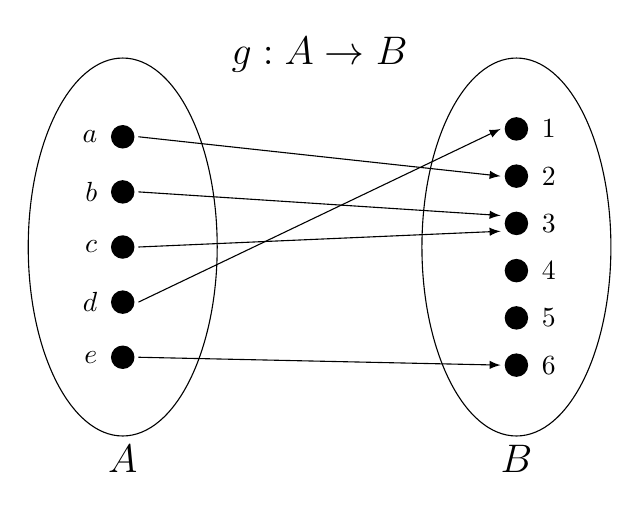
\begin{tikzpicture}[scale=1]
        \foreach \x in  {1,...,6}
        {
            \node at (5, -\x*0.6)[circle,fill,inner sep=3pt]{};
            \draw[shift={(5.2, -\x*0.6)}] node[right] {$\x$};
        }
        \draw (5,-2.1) ellipse (1.2 and 2.4);

        \foreach \x/\s in  {1/a,2/b,3/c,4/d,5/e}
        {
            \node at (0, -\x*0.7)[circle,fill,inner sep=3pt]{};
            \draw[shift={(-0.2, -\x*0.7)}] node[left] {$\s$};
        }
        \draw (0,-2.1) ellipse (1.2 and 2.4);

        \draw[-latex] (0.2,-0.7) -- (4.8,-1.2); 
        \draw[-latex] (0.2,-1.4) -- (4.8,-1.7); 
        \draw[-latex] (0.2,-2.1) -- (4.8,-1.9); 
        \draw[-latex] (0.2,-2.8) -- (4.8,-0.6); 
        \draw[-latex] (0.2,-3.5) -- (4.8,-3.6);
        
        \node[below] at (0, -4.5){\Large $A$};
        \node[below] at (5, -4.5){\Large $B$};
        \node[above] at (2.5, 0){\Large $g:A \to B$};
    \end{tikzpicture}}
\end{center}

然而,这在某种程度上确实\emph{代表}了函数的概念。在这幅图中,我们用椭圆分别表示了定义域 $A$ 和值域 $B$。$A$ 和 $B$ 的元素则用椭圆内的点来表示,并且进行了标记。我们根据函数 $g: A \to B$ 在这些点之间画上箭头。

这种方法通常用于探索函数的特性,或者构造反例来反驳某个主张。通过绘制一些点和箭头,并尝试它们的连接方式,我们可以逐步构建一个例子的基础\emph{结构}。然后,再为图中的各部分分配名称和公式,使其更加严谨。

在我们的讨论中,我们会用一些示意图来说明某些属性和概念,同时提供更严谨的陈述或描述。我们鼓励你也采用这种方法。

% !TeX root = ../../../book.tex

\subsection{习题}

\subsubsection*{温故知新}

以口头或书面的形式简要回答以下问题。这些问题全都基于你刚刚阅读的内容,如果忘记了具体定义、概念或示例,可以回顾相关内容。确保在继续学习之前能够自信地作答这些问题,这将有助于你的理解和记忆!

\begin{enumerate}[label=(\arabic*)]
    \item 在不查阅资料的情况下,写出\textbf{函数}的定义。然后,与我们的定义进行比较。你的定义是否传达了相同的信息?如果没有,遗漏了什么内容?
    \item 函数的\textbf{定义域}和\textbf{值域}有何区别?
    \item 函数\textbf{良好定义}的含义是什么?
    \item 什么是\textbf{恒等函数}?它是如何定义的?
    \item 如何证明两个函数\textbf{相等}?
\end{enumerate}

\subsubsection*{小试牛刀}

尝试解答以下问题。这些题目需动笔书写或口头阐述答案,旨在帮助你熟练运用新概念、定义及符号。题目难度适中,确保掌握它们将大有裨益!

\begin{enumerate}[label=(\arabic*)]
    \item 用符号定义函数:输入整数,输出其绝对值的平方根。\\
          该函数的定义域是什么?值域是什么?
    \item 用符号定义函数:输入一对自然数,输出其算术平均数。\\
          该函数的定义域是什么?值域是什么?
    \item 设 $A = \{-2, -1, 0, 1, 2\}$,定义 $g : A \to A$ 为 $\forall x \in A \centerdot g(x) = x^2 - 3$。绘制示意图来判断 $g$ 是否是良好定义的?
    \item 设 $X$ 为任意集合。用符号定义函数:输入 $X$ 的\emph{子集},输出其在 $X$ 上的补集。\\
          该函数的定义域是什么?值域是什么?
    \item 设 $B = \{-1, 0, 1\}$。定义 $h : B \to B$ 为 $\forall b \in B \centerdot h(b) = b^3$。这与哪个特殊函数相等?
    \item 设 $f : \mathbb{Z} \times \mathbb{Z} \to \mathbb{N}$ 为 $\forall (x, y) \in \mathbb{Z} \times \mathbb{Z} \centerdot f(x, y) = \frac{1}{2}|x + 1| \cdot |y|$。这是一个良好定义的函数吗?为什么?
\end{enumerate}

\newpage
% !TeX root = ../../../book.tex
\section{像与原像}\label{sec:section7.3}

% !TeX root = ../../../book.tex

\subsection{像:定义与示例}

回顾函数的定义,我们要求每个输入都有唯一的输出,这确保了函数在其定义域上的每个元素都有定义。那么值域呢?我们仅要求所有输出都属于值域,但未说明值域的``覆盖程度''。函数的像正是为了描述这一特性。如后续示例所示,即使已知值域,精确确定函数的像也并非总是易事。因此,我们才先定义\emph{函数}及其\emph{值域},再引入\emph{像}的概念。所以请不要误解,我们并不是在有意误导你。

\subsubsection*{定义}

\begin{definition}
    设 $A, B$ 为集合,$f:A \to B$ 为函数,且 $X \subseteq A$。

    \dotuline{$X$ 在函数 $f$ 下的像} 记作 $\im_f(X)$,定义为
    \[\im_f(X) = \{b \in B \mid \exists a \in X \centerdot f(a) = b\}\]
    即 $X$ 在函数 $f$ 下的像是 $X$ 中所有``输入''对应``输出''的集合。

    等价定义为
    \[\im_f(X) = \{f(a) \mid a \in X\}\]
    (当函数明确无歧义时,可简写为 $\im(X)$,并将其称为``$X$ 的像''。)

    当我们说 \dotuline{$f$ 的像}时,指的是整个定义域的像,即 $\im_f (A)$。
\end{definition}

此定义适用于定义域的任意子集 $X \subseteq A$,因此可以讨论定义域的任意``部分''或整体的像。后续示例及练习将涉及 $A$ 的真子集 $X \subset A$ 和全集 $A$。

\subsubsection*{一个发现}

请注意,\emph{对任意} $f, A, B$,恒有
\[\im_f(A) \subseteq B\]
此结论\emph{由定义直接得出},因为像通过 $B$ 的元素构造。下一节将探讨 $\im_f(A) = B$ 的情形。

接下来练习识别函数的像。有时需要验证给定像的正确性,有时需要运用特定方法确定函数的像。

\subsubsection*{示例}

\begin{example}\label{ex:example7.3.2}
    定义函数 $g : A \to B$ 为 $A = \{a, b, c, d, e\}, B = \{1, 2, 3, 4, 5, 6\}$ 且
    \[g = \{(a, 2),(b, 3)(c, 3),(d, 1),(e, 6)\}\]
    设 $X_1 = \{a, b, c\}, X_2 = \{a, c, e\}, X_3 = \{c, d, e\}$。

    你可能已经注意到,此函数与上一节示意图定义的函数相同。参考示意图有助于理解下列像集的计算。

    \begin{center}
        {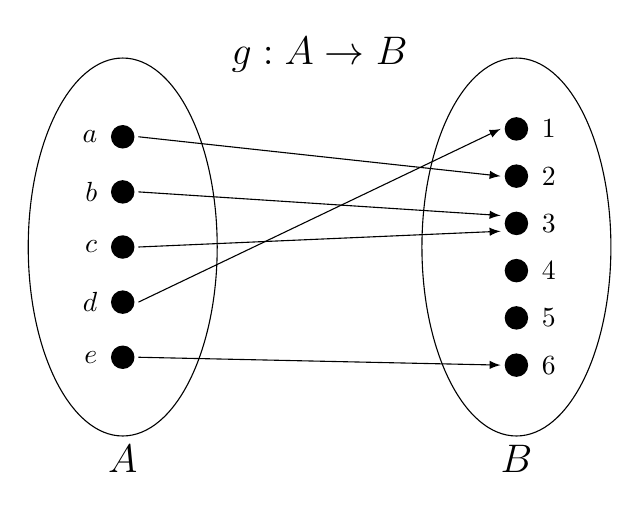
\begin{tikzpicture}[scale=1]
            \foreach \x in  {1,...,6}
            {
                \node at (5, -\x*0.6)[circle,fill,inner sep=3pt]{};
                \draw[shift={(5.2, -\x*0.6)}] node[right] {$\x$};
            }
            \draw (5,-2.1) ellipse (1.2 and 2.4);
    
            \foreach \x/\s in  {1/a,2/b,3/c,4/d,5/e}
            {
                \node at (0, -\x*0.7)[circle,fill,inner sep=3pt]{};
                \draw[shift={(-0.2, -\x*0.7)}] node[left] {$\s$};
            }
            \draw (0,-2.1) ellipse (1.2 and 2.4);
    
            \draw[-latex] (0.2,-0.7) -- (4.8,-1.2); 
            \draw[-latex] (0.2,-1.4) -- (4.8,-1.7); 
            \draw[-latex] (0.2,-2.1) -- (4.8,-1.9); 
            \draw[-latex] (0.2,-2.8) -- (4.8,-0.6); 
            \draw[-latex] (0.2,-3.5) -- (4.8,-3.6);
            
            \node[below] at (0, -4.5){\Large $A$};
            \node[below] at (5, -4.5){\Large $B$};
            \node[above] at (2.5, 0){\Large $g:A \to B$};
        \end{tikzpicture}}
    \end{center}

    \begin{enumerate}[label=(\arabic*)]
        \item $\im_g(\{a\}) = \{2\}$ \\
            请注意此处\emph{大括号}的使用。像永远是\emph{集合}的像,因此写成 $\textcolor{red}{\im_g(a)}$ 是\emph{错误的}。
        \item $\im_g(\{b, c\}) = \{3\}$ \\
            因为 $g(b) = g(c) = 3$。
        \item $\im_g(X_1) = \{2, 3\}$ \\
            因为 $g(b) = g(c) = 3, g(a) = 2$。
        \item $\im_g(X_2) = \{2, 3, 6\}$ \\
            因为 $g(a) = 2, g(c) = 3, g(e) = 6$。
        \item $\im_g(X_3) = \{1, 3, 6\}$ \\
            因为 $g(c) = 3, g(d) = 1, g(e) = 6$。
        \item $\im_g(A) = \{1, 2, 3, 6\}$ \\
            观察示意图中的集合 $B$,可以发现这些值是唯一被函数``命中''的。注意,虽然 $4,5 \in B$,但 $4,5 \notin \im_g(A)$,因此 $\im_g(A) \subset B$,即 $\im_g(A)$ 是 $B$ 的\emph{真}子集)。
    \end{enumerate}
\end{example}

\begin{example}
    考虑液态水的温度范围(以摄氏度为单位)。具体来说,定义集合
    \[C = \{x \in \mathbb{R} \mid 0 < x < 100\}\]
    以及函数 $F : C \to \mathbb{R}$
    \[\forall c \in C \centerdot F(c) = \frac{9}{5}c + 32\]
    $\im_F (C)$ 是什么?其物理意义是什么?

    要解决此问题,我们需要
    \begin{enumerate}[label=(\alph*)]
        \item 通过定义集合来\emph{声明} $\im_F (C)$ 的含义;
        \item 证明该集合\emph{等于} $\im_F (C)$;即二者在集合意义上相等。 
    \end{enumerate}
    
    为此,我们将采用\emph{双向包含论证法}!

    \textbf{解}:定义 $S = \{y \in \mathbb{R} \mid 32 < y < 212\}$。(注意,这表示液态水的温度范围,以华氏度为单位。)我们声称 $S = \im_F(C)$。

    \begin{center}
        \begin{tikzpicture}
            \begin{axis}[
                ymin=0,
                ymax=220,
                xmin=0, 
                xmax=105,
                minor tick num=5,
                axis lines*=middle,
                xtick align=inside,
                ytick align=inside
                ]       
                \addplot[blue, line width=1pt, domain=0:100, samples=2] {x*1.8+32};
            \end{axis}
        \end{tikzpicture}
    \end{center}

    一般来说,很难给出如何提出这种主张的建议。这需要对函数进行一些尝试,可能还需要对其性质有深入洞察。在此例中,我们注意到函数是递增的,即若两个输入值 $c_1 < c_2$,则 $F(c_1) < F(c_2)$。这一结论可从函数图像(见上图)得出,或通过识别其为线性多项式得到。因此,为了确定值域只需计算最小输入值和最大输入值的输出:
    \[F(0) = 0 + 32 = 32 \qquad F(100) = \frac{900}{5} + 32 = 212\]
    由此定义集合 $S$(注意:由于 $0 \notin C$ 不在定义域内,不等式中必须使用``$<$'')。我们特意命名该集合以便后续引用,避免隐含假设其为函数的像——这是微妙而重要的区别!现在,我们来证明该主张。

    \begin{proof}
        首先,证明 $I\im_F (C) \subseteq S$。(即证明函数 $F$ 的每一个输出实际上都满足 $S$ 定义中的不等式。)

        (为此,我们将从 $\im_F (C)$ 的任意元素出发,利用像的\emph{定义}来引入\emph{定义域}中的元素。)

        设 $y \in \im_F (C)$ 为任意固定元素。根据像的定义,这意味着 $\exists x \in C$ 满足 $F(x) = y$。给定这样的 $x$。

        由 $C$ 的定义可知 $ 0 < x < 100$。由 $F$ 的定义可知 $F(x) = \frac{9}{5}x + 32$。由于乘以一个\emph{正数}对加法不会改变不等号的方向,因此可以推导出
        \[ \frac{9}{5} \cdot 0 + 32 < F(x) <  \frac{9}{5} \cdot 100 + 32\]
        化简后得
        \[32 < F(x) < 212\]
        因此,$F(x) \in S$,即 $y \in S$。故 $\im_F(C) \subseteq S$。\\
        
        接着,证明 $S \subseteq \im_F (C)$。(即证明 $S$ 的每一个元素实际上都通过某种方式由函数 $F$ 得到。这相当于证明一个存在性命题,即定义域中存在某个元素。)

        设 $s \in S$ 为任意固定元素。由 $S$ 的定义可知 $S \in \mathbb{R}$ 且 $32 < s < 212$。我们需要证明 $\exists c \in C \centerdot F(c) = s$。

        (通过一些演算可以很容易完成。我们提出了以下思路:只需用 $s$ 表达 $c$ 并求解 $c$……)

        定义 $c = \frac{5}{9}(s-32)$。

        我们要证明 $c \in C$。利用 $s$ 的已知信息并带入不等式,可得
        \begin{align*}
            32 < s < 212 &\implies 0 < s - 32 < 180 \\
            &\implies 0 < \frac{5}{9}(s - 32) < \frac{5}{9} \cdot 180 = 100 \\
            &\implies 0 < c < 100
        \end{align*}

        因为 $c \in \mathbb{R}$,因此 $c \in C$。

        接下来我们证明 $F(c) = s$。不难发现
        \begin{align*}
            F(c) &= \frac{9}{5}c + 32 = \frac{9}{5}\Big(\frac{5}{9}(s-32)\Big)+32\\
            &= (s - 32) + 32 = s
        \end{align*}

        这证明了 $s \in \im_F (C)$,因此 $S \subseteq \im_F (C)$。\\

        综上,利用双向包含论证,我们得到结论 $S = \im_F (C)$。
    \end{proof}
\end{example}

上面证明的后半部分确实较为复杂,这在类似证明中很常见。在选择候选值 $c$ 时,我们本质上需要``逆转''函数 $F$ 的过程,即根据给定输出 $s$ 寻找输入 $c$。当函数涉及实数的数值运算时,最佳方法是建立目标等式,例如
\[\frac{9}{5}c + 32 = s\]
并通过求解得到 $c$。由于该函数是线性的,此过程仅产生唯一的 $c$ 值;但在一般情况下,可能会得到多个符合条件的候选值。完成证明仅需一个有效值,因此任选其一即可。不过,寻找候选值的难度取决于具体问题:有时函数并非定义在数集上,此时需要借助更抽象的思路构造候选元素。总之,一切都取决于具体情况,多加练习便能驾轻就熟!

回到这个像代表什么这个问题,由于定义域表示液态水的摄氏温度,因此像实际上对应液态水的华氏温度。

再考察一个证明函数的像属于特定集合的例子。\\

\begin{example}
    定义 $f : \mathbb{R} \to \mathbb{R}$ 为
    \[\forall x \in \mathbb{R} \centerdot f(x) = \frac{x^2}{1+x^2}\]
    让我们来确定函数的像 $\im_f (\mathbb{R})$,并证明结论!

    在这里,我们需要再次借助一些外部策略和直觉来识别函数的像。我们可以使用微积分或代数方法来绘制该函数的图像,然后试着猜测出函数的像。如果你愿意,可以试试。最终你会得到如下函数图像:

    \begin{center}
        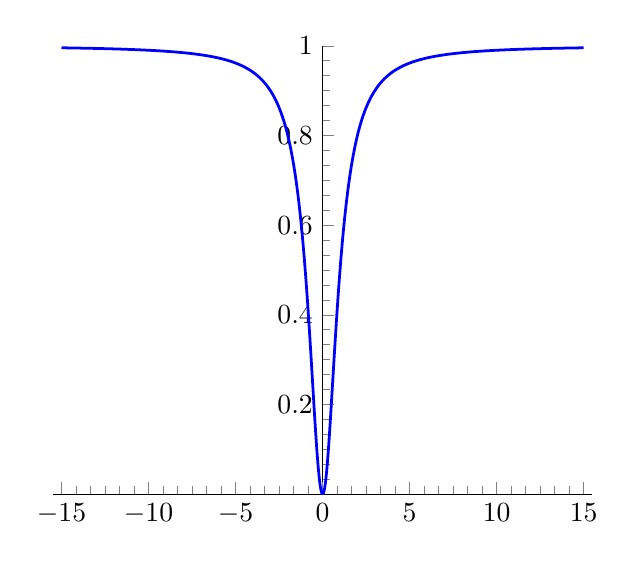
\begin{tikzpicture}
            \begin{axis}[
                ymin=0,
                ymax=1,
                xmin=-15.5, 
                xmax=15.5,
                minor tick num=5,
                axis lines*=middle,
                xtick align=inside,
                ytick align=inside,
                extra x ticks={0}
                ]       
                \addplot[blue, line width=1pt, domain=-15:15, samples=300, smooth] {x^2/(1+x^2)};
            \end{axis}
        \end{tikzpicture}
    \end{center}

    不难发现,表达式中分母大于分子。因此,当 $x$ 越来越大时,分子分母相对来说会越来越接近(也就是说,它们的比率接近 $1$)。另外,由于这两项都涉及平方,因此它们都非负,其比率至少为 $0$。综上所述,我们可以得出以下结论:
    \begin{itemize}
        \item 分母恒大于分子,故当 $|x|$ 增大时,函数值趋近于 $1$
        \item 分子分母均非负,故函数值非负
    \end{itemize}
    据此定义集合
    \[T = \{y \in \mathbb{R} \mid 0 \le y < 1\}\]
    并断言 $T = \im_f(\mathbb{R})$。

    沿用前例证明策略。根据前例的经验,证明所声明集合是像的子集(即 $T \subseteq \im_f (\mathbb{R})$)是难点所在。为此需要处理任意元素 $y \in T$,并寻找 $x \in \mathbb{R}$ 使得 $f(x) = y$。建立如下方程并求解 $x$:
    \begin{align*}
        y = \frac{x^2}{1+x^2} &\iff  (1 + x^2)y = x^2 \\
        &\iff y + yx^2 - x^2 = 0 \\
        &\iff (y - 1)x^2 = -y \\
        &\iff x^2=\frac{y}{1-y} 
    \end{align*}
    求解时需要考虑几个关键问题,$\frac{y}{1-y} \in \mathbb{R}$ 吗?是否确定其非负从而保证 $x$ 存在?如何处理可能出现的双根情况?建议先尝试独立完成证明,再参阅下文给出的证明。

    \begin{proof}
        首先,证明 $\im_f (\mathbb{R}) \subseteq T$。

        设 $y \in \im_f (\mathbb{R})$ 为任意固定元素。根据像的定义,$\exists x \in \mathbb{R}$ 使得 $f(x) = y$。给定这样的 $x$。

        由 $x \in \mathbb{R}$ 可知 $x^2 \ge 0$ 且 $0 < x^2+1$,由此可得 $0 < \frac{1}{x^2+1}$。

        由于所有项均非负,将 $0 < x^2+1$ 和 $0 < \frac{1}{x^2+1}$ 相乘得 $0 < \frac{x^2}{1+x^2}$。

        又由 $0 \le x^2 < x^2 + 1$,可得 $\frac{x^2}{x^2+1}<1$。(备注,为什么指出 $x^2>0$ 很重要?不指出可能会出现什么问题?)

        这证明了 $0 \le \frac{x^2}{1+x^2} < 1$。因为 $y = f(x) = \frac{x^2}{1+x^2}$,这等价于 $0 \le y < 1$。

        故 $y \in T$,因此 $\im_f (\mathbb{R}) \subseteq T$。\\

        接着,证明 $T \subseteq \im_f (\mathbb{R})$。

        设 $y \in T$ 为任意固定元素。这意味着 $y \in \mathbb{R}$ 且 $0 \le y < 1$。

        要证明 $y \in \im_f (\mathbb{R})$,需要得到一个 $x$ 满足 $f(x) = y$。

        我们声称 $x = \sqrt{\frac{y}{1-y}}$ 满足。

        请注意 $0 \le y < 1 \implies -y > -1$,所以 $1-y > 0$。由于 $\frac{y}{1-y} \ge 0$ 且 $x \in \mathbb{R}$,因此可以明确定义为平方根,且 $x$ 属于定义域 $\mathbb{R}$。
        
        注意到 $x^2=\frac{y}{1-y}$,所以
        \[f(x) = \frac{x^2}{1+x^2} = \frac{\frac{y}{1-y}}{1+\frac{y}{1-y}}=\frac{\frac{y}{1-y}}{\frac{(1-y)+y}{1-y}}=\frac{\frac{y}{1-y}}{\frac{1}{1-y}}=\frac{y}{1-y} \cdot \frac{1-y}{1} = \frac{y}{1} = y\]

        这证明了 $y \in \im_f (R)$,因此 $T \subseteq \im_f (R)$。\\

        综上,利用双向包含论证,我们得到结论 $T = \im_f (\mathbb{R})$。
    \end{proof}
\end{example}

请注意我们如何解决先前讨论的证明问题:存在两个可行的 $x$ 值(正平方根与负平方根),但我们仅需一个,这里选择正平方根并完成证明。

(问题:若函数仅定义在非负实数上会怎样?仅定义在负实数上呢?这些限制如何影响我们的选择?)\\

\begin{example}
    考虑函数 $p:\mathbb{N} \times \mathbb{N} \to \mathbb{N}$ 定义为
    \[\forall (a, b) \in \mathbb{N} \times \mathbb{N} \centerdot p(a, b) = ab + a\]
    $\im_p(\mathbb{N})$ 是什么?

    此例可能稍显复杂,因为它涉及集合的笛卡尔积,即函数 $p$ 以自然数对为输入并输出自然数。在这种情况下,一个有效策略是先代入一些具体值观察规律,如下表所示,其中左列为 $a$,顶行为 $b$,表格中的值为 $p(a,b)$。

    \begin{center}
        \begin{tabular}{c|ccccc}
              &  1 &  2 &  3 &  4 &  5 \\
            \hline
            1 &  2 &  3 &  4 &  5 &  6 \\
            2 &  4 &  6 &  8 & 10 & 12 \\
            3 &  6 &  9 & 12 & 15 & 18 \\
            4 &  8 & 12 & 16 & 20 & 24 \\
            5 & 10 & 15 & 20 & 25 & 30 \\
        \end{tabular}
    \end{center}

    看起来函数 $p$ ``取得''除 $1$ 以外的所有自然数。特别地,数组第一行显示除 $1$ 以外所有自然数均出现。下文证明将运用这一洞察。

    \begin{proof}
        设 $V = N - \{1\}$。我们声称 $V = \im_p(\mathbb{N} \times \mathbb{N})$。

        首先,证明 $\im_p(\mathbb{N} \times \mathbb{N}) \subseteq V$。

        设 $n \in \im_p(\mathbb{N} \times \mathbb{N})$ 为任意固定元素。这意味着 $n \in \mathbb{N}$ 且 $\exists (a,b) \in \mathbb{N} \times \mathbb{N}$ 使得 $p(a,b)=n$。给定这样的 $(a,b)$。这意味着 $n=ab+a$。
        
        由 $a,b \ge 1$ 可得 $ab \ge 1$,因此 $n = ab + a \ge 2$。根据 $V$ 的定义,这证明了 $n \in V$。

        因此 $\im_p(\mathbb{N} \times \mathbb{N}) \subseteq V$。

        (在继续阅读之前,试着自己写出证明的后半部分!)\\

        接着,证明 $V \subseteq \im_p(\mathbb{N} \times \mathbb{N})$。

        设 $v \in V$ 为任意固定元素。这意味着 $v \in \mathbb{N}$ 且 $v \ge 2$。定义 $(a, b) = (v - 1, 1)$。

        注意到 $v - 1 \ge 1$,故 $v-1 \in \mathbb{N}$,所以 $(a, b) \in \mathbb{N} \times \mathbb{N}$。

        此外,我们还注意到
        \[p(a, b) = p(v - 1, 1) = (v - 1) \centerdot 1 + 1 = v - 1 + 1 = v\]
        
        故 $p(a, b) = v$,所以 $(a,b) \in \im_p(\mathbb{N} \times \mathbb{N})$。
        
        因此 $V \subseteq \im_p(\mathbb{N} \times \mathbb{N})$。\\

        综上,利用双向包含论证,我们得到结论 $V = \im_p(\mathbb{N} \times \mathbb{N})$。
    \end{proof}
\end{example}

% !TeX root = ../../../book.tex

\subsection{关于像的证明}

你可能已经通过研究我们之前看到的一些例子发现了以下事实。无论如何,我们都可以通过使用像的定义来陈述和证明这个命题。请注意,这是关于\emph{任意}函数的命题;无论 $f$ 是什么,它都成立!

\begin{proposition}\label{prop:proposition7.3.6}
    设 $A,B$ 为集合,$f:A \to B$ 为函数。设 $S, T \subseteq A$,则
    \[Im_f (S \cap T) \subseteq Im_f (S) \cap Im_f (T)\]
\end{proposition}

\begin{proof}
    设 $z \in Im_f (S \cap T)$ 为任意固定元素。这意味着 $\exists a \in S \cap T$ 使得 $f(a) = z$。给定这样的 $a$。

    因为 $a \in S \cap T$,所以我们知道 $a \in S$ 且 $a \in T$。

    因此,根据像的定义,$z \in Im_f (S)$ 且 $z \in Im_f (T)$。

    根据交集的定义,我们推导出 $z \in Im_f (S) \cap Im_f (T)$。

    这证明了我们要证明的集合包含关系。
\end{proof}

为什么我们没有在这里声明\emph{相等}呢?实际上,相等\emph{不一定成立}!也就是说,存在至少一个函数使得逆包含关系 --- 即 $Im_f (S) \cap Im_f (T) \subseteq Im_f (S \cap T)$ --- 不成立。我们将在下面提供这样一个函数的例子。

(你应该尝试想出一个逆包含关系\emph{成立}的函数的例子。这样,我们就能证明不能\emph{必然}得出这个包含关系成立的结论!)

我们将通过示意图来展示一个具有特定属性的例子。然后,我们会使用这个例子来正式\emph{定义}一个函数,并说明其属性,指出这些属性如何与我们的论点相一致。

需要注意的是,使用这种方法是完全可行的,只要你之后补充一个正式的定义。仅仅依靠示意图作为``证明''是不够严谨的,但它确实能帮助你更好地构思证明的\emph{思路}。

另外,在这种情况下,没有必要构造\emph{复杂}或\emph{有趣}的反例。如果你想\emph{反驳}一个全称量化陈述,只需要\emph{一个}有效的例子就可以了!特别是,不要觉得你需要定义一个通过\emph{公式}处理\emph{数字}的函数。有时,这反而会增加难度!通常,反例可以通过只包含几个(如两个或三个)元素的集合来构造。\\

\begin{example}
    我们声称存在集合 $A,B,S,T$ 和函数 $f : A \to B$,使得 $Im_f (S) \cap Im_f (T) \nsubseteq Im_f (S \cap T)$。让我们看看如何构造这样的例子。基于前面的讨论,我们将尝试构造一个包含大约三个元素的集合的例子。我们先令 $A = \{1, 2, 3\}$ 并定义 $f(1)$:

    \begin{center}
        {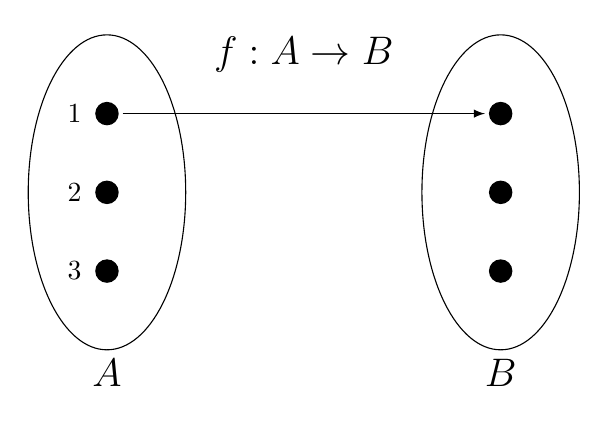
\begin{tikzpicture}[scale=1]
            \foreach \x in  {1,2,3}
            {
                \node at (5, -\x)[circle,fill,inner sep=3pt]{};
            }
            \draw[shift={(5.2, -1)}] node[right] {$\bigstar$};
            \draw (5,-2) ellipse (1 and 2);
    
            \foreach \x in  {1,2,3}
            {
                \node at (0, -\x)[circle,fill,inner sep=3pt]{};
                \draw[shift={(-0.2, -\x)}] node[left] {$\x$};
            }
            \draw (0,-2) ellipse (1 and 2);
    
            \draw[-latex] (0.2,-1) -- (4.8,-1); 
            
            \node[below] at (0, -4){\Large $A$};
            \node[below] at (5, -4){\Large $B$};
            \node[above] at (2.5, -0.6){\Large $f:A \to B$};
        \end{tikzpicture}}
    \end{center}

    为了便于定义,我们令 $S = \{1, 2\}$。让 $S$ 中包含两个元素似乎更合理,因此我们做出这个选择。此外,我们应该设 $f(1) \ne f(2)$,否则 $Im_f(S)$ 只会包含一个元素,这样 $S$ 有两个元素就没有意义了。因此,我们定义 $f(2)$:

    \begin{center}
        {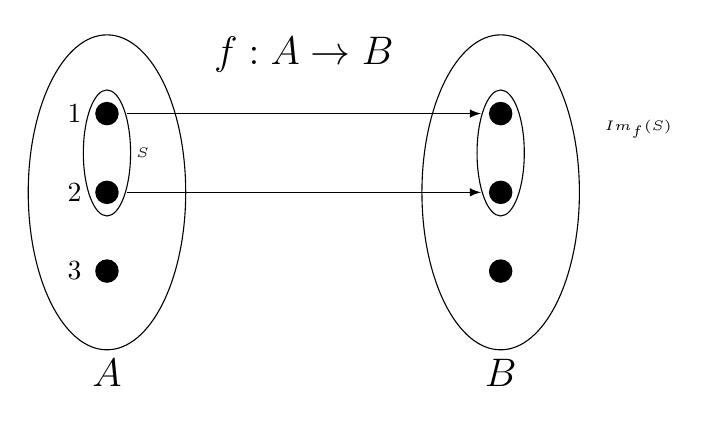
\begin{tikzpicture}[scale=1]
            \foreach \x in  {1,2,3}
            {
                \node at (5, -\x)[circle,fill,inner sep=3pt]{};
            }
            \draw[shift={(5.2, -1)}] node[right] {$\bigstar$};
            \draw[shift={(5.2, -2)}] node[right] {$\square$};
            \draw (5,-2) ellipse (1 and 2);
            \draw (5,-1.5) ellipse (0.3 and 0.8);
    
            \foreach \x in  {1,2,3}
            {
                \node at (0, -\x)[circle,fill,inner sep=3pt]{};
                \draw[shift={(-0.2, -\x)}] node[left] {$\x$};
            }
            \draw (0,-2) ellipse (1 and 2);
            \draw (0,-1.5) ellipse (0.3 and 0.8);
    
            \draw[-latex] (0.25,-1) -- (4.75,-1);
            \draw[-latex] (0.25,-2) -- (4.75,-2); 
    
            \node[right] at (0.25, -1.5){\tiny $S$};
            \node[right] at (6.2, -1.2){\tiny $Im_f(S)$};
            \node[below] at (0, -4){\Large $A$};
            \node[below] at (5, -4){\Large $B$};
            \node[above] at (2.5, -0.6){\Large $f:A \to B$};
        \end{tikzpicture}}
    \end{center}

    现在,我们需要选择集合 $T$。如果让 $S$ 和 $T$ 互不相交 ($S \cap T = \varnothing$) 会很有趣,而如果让 $T$ 包含 $S$ ($T \supseteq S$),处理起来可能会很复杂。因此,我们设 $T = \{2, 3\}$。接下来,我们只需要定义 $f(3)$。在考虑每种情况时,请参照上面的示意图,想象画一个箭头来表示 $f(3)$。

    \begin{itemize}
        \item 如果 $f(3) = f(2) = \square$。\\
            这种情况下,$Im_f(T) = \{\square\}$,所以 $Im_f (S) \cap Im_f (T) = \{\square\}$。而 $Im_f (S \cap T) = \{\square\}$, 这行不通。
        \item 如果 $f(3)$ 等于其他值,比如 $\smiley{}$。\\
            这也行不通。我们会得到 $Im_f (S) \cap Im_f (T) = \{\square\} = Im_f (S \cap T)$。
        \item 如果 $f(3) = f(1) = \bigstar$。\\
            这似乎可以!
    \end{itemize}

    \begin{center}
        {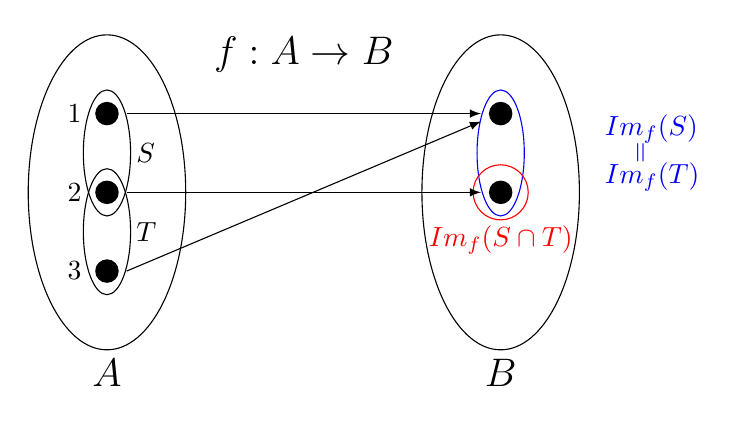
\begin{tikzpicture}[scale=1]
            \foreach \x in {1,2}
            {
                \node at (5, -\x)[circle,fill,inner sep=3pt]{};
            }
            \draw[shift={(5.2, -1)}] node[right] {$\bigstar$};
            \draw[shift={(5.2, -2)}] node[right] {$\square$};
            \draw (5,-2) ellipse (1 and 2);
            \draw[blue] (5,-1.5) ellipse (0.3 and 0.8);
            \draw[red] (5,-2) circle (0.35);
            \node[below, red] at (5, -2.3){$Im_f(S \cap T)$};
    
            \foreach \x in  {1,2,3}
            {
                \node at (0, -\x)[circle,fill,inner sep=3pt]{};
                \draw[shift={(-0.2, -\x)}] node[left] {$\x$};
            }
            \draw (0,-2) ellipse (1 and 2);
            \draw (0,-1.5) ellipse (0.3 and 0.8);
            \draw (0,-2.5) ellipse (0.3 and 0.8);
    
            \draw[-latex] (0.25,-1) -- (4.75,-1);
            \draw[-latex] (0.25,-2) -- (4.75,-2); 
            \draw[-latex] (0.25,-3) -- (4.75,-1.1); 
    
            \node[right] at (0.25, -1.5){$S$};
            \node[right] at (0.25, -2.5){$T$};
            \node[right, blue] at (6.2, -1.2){$Im_f(S)$};
            \node[right, blue, anchor=center, rotate=90] at (6.8, -1.5){$=$};
            \node[right, blue] at (6.2, -1.8){$Im_f(T)$};
            \node[below] at (0, -4){\Large$A$};
            \node[below] at (5, -4){\Large$B$};
            \node[above] at (2.5, -0.6){\Large $f:A \to B$};
        \end{tikzpicture}}
    \end{center}
\end{example}

我们已经成功实现 $Im_f (S) \cap Im_f (T)$ 是 $Im_f (S \cap T)$ 的\emph{真}超集。

回顾一下我们的构造过程,看看你是否理解我们的思路。我们需要遵守哪些限制?在哪些方面有选择的自由?我们最终决定怎么做?

需要说明的是,这绝对不是\emph{唯一的}例子!你也可以尝试想出其他的例子!

现在,我们只需要用我们构造的最终示意图来定义一个例子,并证明它的有效性。我们开始吧!

\begin{proof}
    定义 $A = \{1, 2, 3\}, B = \{\bigstar, \square\}$。

    定义 $f : A \to B$ 为 $f(1) = \bigstar, f(2) = \square, f(3) = \bigstar$。

    定义 $S = \{1, 2\}, T = \{2, 3\}$。

    易得 $S \cap T = \{2\}$,所以 $Im_f (S \cap T) = \{f(2)\} = \{\square\}$。

    然而,$Im_f (S) = Imf (T) = B$,所以 $Im_f (S) \cap Im_f (T) = \{\bigstar, \square\} \ne \{\square\}$。

    因为 $\bigstar \in Im_f (S) \cap Im_f (T)$ 而 $\bigstar \notin Im_f (S \cap T)$,这证明了我们的声明。
\end{proof}

我们已经展示了如何\textbf{证明}关于任意函数和像的声明,以及如何通过\textbf{构造}具体反例来\textbf{反驳}一个声明。在下面的练习中,你将会遇到类似的问题。有时,你需要判断一个声明是否为真。(在这里,我们已经提前告诉你哪个声明是正确的。)我们建议你可以尝试以下两种方法:
\begin{enumerate}[label=(\arabic*)]
    \item 试着证明这个声明,看看是否在某个地方会出现问题;
    \item 试着构造一个反例,看看是否会遇到困难。
\end{enumerate}
如果你完成了上面任意一项……太好了,你已经解决了这个问题!但如果你感到困难,这可能会帮助你更好地理解问题的本质。

具体来说,我们要求你用 ``$\cup$'' 代替 ``$\cap$'' 来重新审视我们上面讨论的命题。你认为会有什么不同吗?试试看吧!

% !TeX root = ../../../book.tex

\subsection{原像:定义与示例}

你可能会问:那反过来呢?我们能否取值域的一个子集,然后找出哪些定义域中的元素的输出落在该子集中?当然可以!接下来的定义将为这一概念提供一个术语,你会发现它与``像''的定义有很多相似之处。

\subsubsection*{定义}

\begin{definition}
    设 $A, B$ 为集合,$f:A \to B$ 为函数。设 $Y \subseteq B$。

    \dotuline{$Y$ 在函数 $f$ 下的原像} 写做 $PreIm_f(Y)$,定义为
    \[PreIm_f (Y) = \{a \in A \mid f(a) \in Y \}\]
    也就是说,$Y$ 在函数 $f$ 下的原像是所有能产生 $Y$ 中``输出''的``输入''的集合。

    (当函数明确且无歧义时,我们有时会将符号简写为 $PreIm(Y)$,并将其称为 ``$Y$ 的原像'',而不是``$Y$ 在函数 $f$ 下的原像''。)
\end{definition}

首先思考一下:什么是 $PreIm_f (B)$?这里 $B$ 是整个值域。

回顾一下定义:$PreIm_f (B)$ 是所有输入 (在 $A$ 中) 的集合,这些输入的输出``落''在 $B$ 上。由于 $f$ 是一个良好定义的函数,所以 $PreIm_f (B)$ 实际上就是整个 $A$。因此,我们通常只会关注 $Y \subset B$ 的情况,因为这些情况更有趣。

\subsubsection*{示例}

\begin{example}
    第一个例子沿用了我们在上一节中讨论图时定义的函数。我们会再次展示示意图,但不会重新定义函数的所有细节。(详细信息请参见示例 \ref{ex:example7.3.2}。)

    \begin{center}
        {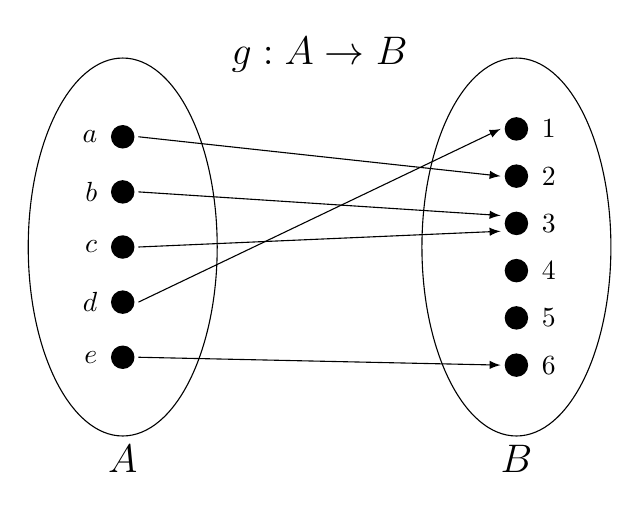
\begin{tikzpicture}[scale=1]
            \foreach \x in  {1,...,6}
            {
                \node at (5, -\x*0.6)[circle,fill,inner sep=3pt]{};
                \draw[shift={(5.2, -\x*0.6)}] node[right] {$\x$};
            }
            \draw (5,-2.1) ellipse (1.2 and 2.4);
    
            \foreach \x/\s in  {1/a,2/b,3/c,4/d,5/e}
            {
                \node at (0, -\x*0.7)[circle,fill,inner sep=3pt]{};
                \draw[shift={(-0.2, -\x*0.7)}] node[left] {$\s$};
            }
            \draw (0,-2.1) ellipse (1.2 and 2.4);
    
            \draw[-latex] (0.2,-0.7) -- (4.8,-1.2); 
            \draw[-latex] (0.2,-1.4) -- (4.8,-1.7); 
            \draw[-latex] (0.2,-2.1) -- (4.8,-1.9); 
            \draw[-latex] (0.2,-2.8) -- (4.8,-0.6); 
            \draw[-latex] (0.2,-3.5) -- (4.8,-3.6);
            
            \node[below] at (0, -4.5){\Large $A$};
            \node[below] at (5, -4.5){\Large $B$};
            \node[above] at (2.5, 0){\Large $g:A \to B$};
        \end{tikzpicture}}
    \end{center}

    定义 $Z_1 = \{1, 2, 3\}, Z_2 = \{2, 3, 4\}, Z_3 = \{4, 5, 6\}$。

    让我们识别并解释以下原像。

    \begin{enumerate}[label=(\arabic*)]
        \item $PreIm_g(\{1\}) = \{d\}$ \\
            因为 $g(d) = 1$ 且没有其他 $x \in A$ 满足 $g(x) = 1$。\\
            (注意,这里需要使用\emph{大括号}。``$PreIm_g(1)$'' 是没有意义的。)
        \item $PreIm_g(\{4\}) = \varnothing$ \\
            因为没有 $x \in A$ 满足 $g(x) = 4$。
        \item $PreIm_g(Z_1) = \{a, b, c, d\}$ \\
            因为 $g(a) = 2, g(b) = g(c) = 3, g(d) = 1$,但没有其他 $x \in A$ 满足 $g(x) \in Z_1$。
        \item $PreIm_g(Z_2) = \{a, b, c\}$ \\
            因为 $g(a) = 2, g(b) = g(c) = 3$,但没有其他 $x \in A$ 满足 $g(x) \in Z_2$。
        \item $PreIm_g(Z_3) = \{e\}$ \\
            因为 $g(e) = 6$,但没有其他 $x \in A$ 满足 $g(x) \in Z_3$。
        \item $PreImg(\{5\}) = \varnothing$ \\
            因为 $\forall x \in A \centerdot g(x) \ne 5$。
    \end{enumerate}
\end{example}

\begin{example}
    设函数 $f : \mathbb{R} \to \mathbb{R}$ 定义为 $\forall x \in \mathbb{R} \centerdot f(x) = x^2$。

    现在我们用这个函数来找几个原像。这次,我们希望你自己弄清楚为什么我们的结论是正确的,并尝试解释和证明它们。

    \begin{enumerate}[label=(\arabic*)]
        \item $PreIm_f (\{1\}) = \{-1, 1\}$
        \item $PreIm_f (\{y \in \mathbb{R} \mid y < 0\}) = \varnothing$
        \item $PreIm_f (\{y \in \mathbb{R} \mid y \ge 0\}) = \mathbb{R}$
        \item $PreIm_f (\{y \in \mathbb{R} \mid 0 < y < 1\}) = \{x \in \mathbb{R} \mid -1 < x < 1\}$
    \end{enumerate}
\end{example}

% !TeX root = ../../../book.tex

\subsection{关于原像的证明}


% !TeX root = ../../../book.tex

\subsection{习题}

\subsubsection*{温故知新}

以口头或书面的形式简要回答以下问题。这些问题全都基于你刚刚阅读的内容,如果忘记了具体定义、概念或示例,可以回顾相关内容。确保在继续学习之前能够自信地作答这些问题,这将有助于你的理解和记忆!

\begin{enumerate}[label=(\arabic*)]
    \item \textbf{像}与\textbf{原像}之间有什么区别?
    \item 假设 $f : A \to B$ 是一个函数。$\pim_f (B)$ 表示什么?
    \item 假设 $g : \mathbb{R} \to \mathbb{R}$ 是一个函数。为什么表达式 $\im_g(0)$ 不是一个正确的陈述?你认为写出该表达式的人想表达什么意思?
    \item 假设 $f : A \to B$ 是一个函数且 $Y \subseteq B$。如果 $\pim_f (Y) = \varnothing$,这意味着什么?这有可能吗?
    \item 假设 $f : A \to B$ 是一个函数且 $X \subseteq A$。如果 $\im_f (X) = \varnothing$,这意味着什么?这有可能吗?
\end{enumerate}

\subsubsection*{小试牛刀}

尝试解答以下问题。这些题目需动笔书写或口头阐述答案,旨在帮助你熟练运用新概念、定义及符号。题目难度适中,确保掌握它们将大有裨益!

\begin{enumerate}[label=(\arabic*)]
    \item 设函数 $h : \mathbb{R} - \{-1\} \to \mathbb{R}$ 定义为 $\forall x \in \mathbb{R} - \{-1\} \centerdot h(x) = \frac{x}{1+x}$。\\
        证明 $\im_h(\mathbb{R} - \{-1\}) = \mathbb{R} - \{-1\}$。\\
        然后,定义 $P = \{y \in \mathbb{R} \mid y > 1\}, U = \{y \in \mathbb{R} \mid y > -1\}$。 \\
        证明 $\pim_h(P) = U$。
    \item 设 $f:A \to B$ 为函数。设 $S,T \subseteq A$。对于下列陈述,\textbf{证明}其成立,或找出\textbf{反例}。
        \begin{enumerate}[label=(\alph*)]
            \item $\im_f (S \cup T) \subseteq \im_f (S) \cup \im_f (T)$
            \item $\im_f (S \cup T) \supseteq \im_f (S) \cup \im_f (T)$
        \end{enumerate}
    \item 设 $f:A \to B$ 为函数。设 $Y,Z \subseteq B$。对于下列陈述,\textbf{证明}其成立,或找出\textbf{反例}。
        \begin{enumerate}[label=(\alph*)]
            \item $\pim_f (Y \cup Z) \subseteq \pim_f (Y) \cup \pim_f (Z)$
            \item $\pim_f (Y \cup Z) \supseteq \pim_f (Y) \cup \pim_f (Z)$
        \end{enumerate}
    \item 回看命题 \ref{prop:proposition7.3.12},考虑\emph{反方向}包含关系
        \[\im_f \big(\pim_f (Y)\big) \supseteq Y\]
        通过构造一个具体的反例并证明其有效性,来\textbf{反驳}以下陈述:对于任意函数 $f : A \to B$ 和任意 $Y \subseteq B$,该陈述都成立。
\end{enumerate}

\newpage
% !TeX root = ../../../book.tex

\section{函数的性质}

% !TeX root = ../../../book.tex

\subsection{满射函数}

你可能会问……如果我们能确定给定函数定义域的像,为什么还要用比这个像更大的值域呢?例如,函数 $f : \mathbb{R} \to \mathbb{R}$ 定义为 $f(x) = x^2$ 是良好定义的函数,但如果把值域改为非负实数集也不会有任何影响。这样做甚至更好,因为函数不会``遗漏''任何值域中的元素!如果你有这样的想法,那么你已经理解了我们接下来的定义,这个定义准确地概括了函数的这一特性:值域和定义域的像是同一个集合这种情况。

\subsubsection*{定义}

\begin{definition}
    设 $A,B$ 为集合,$f:A \to B$ 为函数。我们说 $f$ 是\dotuline{满射}函数,当且仅当 $Im_f (A) = B$。

    同样地,我们可以说 ``$f$ 是满射的''(形容词形式),或者说 ``$f$ 是一个满射''(名词形式)。

    回到像的定义,我们可以用一个量化陈述来等价地描述这个性质:
    \[f \;\text{是满射} \iff \forall b \in B \centerdot \exists a \in A \centerdot f(a) = b\]
    也就是说,$f$ 是满射当且仅当每个输出至少有一个对应的输入。
\end{definition}

想一想为什么这个定义的第二种形式实际上与第一种形式是相同的。性质 $Im_f (A) = B$ 是关于集合的陈述。根据定义,我们已经知道 $Imf (A) \subseteq B$(像中的任何元素都不能``超出''值域),所以这个进一步的性质意味着 $B \subseteq Im_f (A)$。这正是定义的第二种形式所说的:值域的每个元素都满足像元素的定义。

另外,注意定义中没有说我们找到的与 $b$ 对应的 $a$ 必须是唯一的!这个性质所要求的只是,对于每个 $b \in B$,我们可以找到\emph{至少一个} $a \in A$ 满足 $f(a) = b$。可能有多个,也可能只有一个。这无关紧要,只要不是\emph{一个都没有}就行。

在示意图中,\emph{满射}的性质意味着什么?由于值域的每个元素都被函数``命中'',这意味着示意图右侧的每个点都有一个箭头指向它。(记住:这种启发式语言是可以记住的 --- 毕竟我们用它来帮助描述这些概念 --- 但这不构成证明。在你用于证明的任何语句中,应该使用着更严格的陈述,使用数学语言和/或逻辑符号。)为什么我们会关心这样的性质?一般来说,声明一个函数的像究竟是什么可能很困难,我们可能(首先)只能声明值域是什么。实际上证明值域的所有元素都是函数的输出可以提供额外的、有用的信息!

\subsubsection*{满射定义的否定}

通常,我们会先定义一个函数,然后问:这是一个满射吗?如果我们认为一个函数是满射,我们应该通过证明值域和像是同一集合来证实。如果我们认为它不是满射,我们应该通过找到一个反例来证明它不是满射。让我们来看一下满射函数定义的逻辑否定:
\[\neg (\forall b \in B \centerdot \exists a \in A \centerdot f(a) = b) \iff \exists b \in B \centerdot \forall a \in A \centerdot f(a) \ne b\]
也就是说,要证明函数 $f$ 不是满射,我们必须找到一个不在像中的值域元素。这需要一些验算和直觉来识别这样的元素 $b$。接下来,我们必须以某种方式证明没有任何 $a$ 满足 $f(a) = b$。我们可以通过取任意 $a \in A$ 并解释为什么 $f(a) \ne b$ 来直接证明这一点。或者,我们可以通过反证法来证明:假设存在一个 $a \in A$ 使得 $f(a) = b$,然后找出矛盾。这两种方法都是合理的,并且是逻辑等价的。

\subsubsection*{示例}

让我们通过几个例子来看看这些技术是如何应用的。对于其中一些例子,我们可以借助图形直觉或尝试一些测试案例来进行\emph{猜想},但最终我们需要通过\emph{证明}某些逻辑陈述来验证我们的观点。\\

\begin{example}
    考虑函数 $p : \mathbb{N} \times \mathbb{N} \to \mathbb{N}$ 定义为 $p(a,b) = ab$。$p$ 是满射吗?

    答案是肯定的。我们可以设 $a$ 为 $1$,则函数的输出就是 $b$。让我们通过证明来让这个观察更加正式:

    \begin{proof}
        设 $n \in \mathbb{N}$ 为任意固定自然数。定义 $(a, b) = (1, n)$。

        不难发现 $(1, n) \in \mathbb{N} \times \mathbb{N}$ 且 $p(1, n) = 1 \cdot n = n$。

        因为 $n$ 是任意的,这证明了 $p$ 是满射。
    \end{proof}
\end{example}

\begin{example}
    设 $C$ 为美国所有汽车的集合。设 $S$ 为所有由字母和数字组成的长度最多为 $7$ 的字符串的集合(这些是可能出现在汽车牌照上的\emph{潜在}字符串)。

    设 $f : C \to S$ 定义为输入一辆车,输出其牌照字符串。函数 $f$ 是满射吗?

    不,绝对不是!也许你没注意到,\emph{敏感词}是不允许出现在牌照上的!所以,肯定存在许多在美国牌照上绝对不会出现的字符串。(我们就不列举了,你可以自己想一些例子……)

    因为我们展示了 $S$ 中至少有一个元素\emph{不是} $Im_f (C)$ 的元素,因此我们已经证明了 $f$ 不是一个满射。
\end{example}

\begin{example}
    设函数 $d : \mathbb{N} \times \mathbb{N} \to \mathbb{Z}$ 定义为
    \[\forall (a, b) \in \mathbb{N} \times \mathbb{N} \centerdot d(a, b) = a - b\]
    我们来判断 $d$ 是否是满射,并证明我们的结论。
    
    我们可以先尝试一些``较小的''输入值。在下表中,左列表示 $a$,顶行表示 $b$,表格中的值是 $d(a, b) = a - b$:
    \begin{center}
        \begin{tabular}{c|ccccc}
              &  1 &  2 &  3 &  4 &  5 \\
            \hline
            1 &  0 & -1 & -2 & -3 & -4 \\
            2 &  1 &  0 & -1 & -2 & -3 \\
            3 &  2 &  1 &  0 & -1 & -2 \\
            4 &  3 &  2 &  1 &  0 & -1 \\
            5 &  4 &  3 &  2 &  1 &  0 \\
        \end{tabular}
    \end{center}
    看起来所有的整数 $z \in \mathbb{Z}$ 都会出现在这个表格中。然而,它们不会全部出现在某一特定的行或列中。相反,所有非负整数似乎都出现在第一列,而所有非正整数似乎都出现在第一行。让我们根据这些观察来写一个证明。我们将取任意整数 $z \in \mathbb{Z}$,并分两种情况讨论:如果 $z \ge 0$,我们将采取一种方法;如果 $z < 0$,我们将采取另一种方法。只要我们在这两种情况下都成功,我们就证明了 $d$ 是一个满射。

    \begin{proof}
        我们声称 $d$ 是满射。

        设 $z \in \mathbb{Z}$ 是任意固定整数。我们要证明 $\exists (a, b) \in \mathbb{N} \times \mathbb{N} \centerdot d(a, b) = z$。为此,考虑如下两种情况:
        \begin{enumerate}[label=(\arabic*)]
            \item 假设 $z \ge 0$,则定义 $(a, b) = (z + 1, 1)$。\\
                因为 $z \ge 0$,我们知道 $z+1 \ge 1$,因此 $z+1 \in \mathbb{N}$。这确保了 $(z + 1, 1) \in \mathbb{N} \times \mathbb{N}$。\\
                此时 $d(z + 1, 1) = (z + 1) - 1 = z$。
            \item 假设 $z < 0$,则定义 $ (a, b) = (1, -z + 1)$。\\
                因为 $z < 0$,我们知道 $-z > 0$,因此 $-z+1 > 1$,这意味着 $-z+1 \in \mathbb{N}$。这确保了 $(1, -z+1) \in \mathbb{N} \times \mathbb{N}$。\\
                此时 $d(1, -z + 1) = 1 - (-z + 1) = z$。
        \end{enumerate}
        无论哪种情况,我们都可以定义 $(a, b) \in \mathbb{N} \times \mathbb{N} \centerdot d(a, b) = z$。因为 $z \in \mathbb{Z}$ 是任意整数,所以这证明了 $d$ 是一个满射。
    \end{proof}
\end{example}

\begin{example}
    设函数 $g : \mathbb{R} - \{-1\} \to \mathbb{R}$ 定义为 
    \[\forall x \in \mathbb{R} - \{-1\} \centerdot g(x) = \frac{x}{1+x}\]
    (注意,我们为什么从定义域中移除了 $-1$。这是为了确保 $g$ 是\emph{良好定义的}。)

    我们来判断 $g$ 是否是满射,并证明我们的结论。如前所述,我们可以通过做一些验算来确定这一点:我们可以尝试代入一些 $x$ 的值,让 $x$ 非常接近 $-1$ 或变得越来越大,以测试``极端情况''……这些都有助于我们绘制函数图像,或者我们可以使用绘图软件直接画出函数图像:

    \begin{center}
        \begin{tikzpicture}
            \begin{axis}[
                ymin=-1.5,
                ymax=3.5,
                xmin=-5, 
                xmax=5,
                minor tick num=3,
                axis lines*=middle,
                xtick align=inside,
                ytick align=inside
                ]       
                \addplot[blue, line width=1pt, domain=-5:-1.1, samples=40, smooth] {x/(1+x)};
                \addplot[blue, line width=1pt, domain=-0.9: 5, samples=60, smooth] {x/(1+x)};
                \addplot[black, dashed, domain=-5:5, samples=2] {1};
            \end{axis}
        \end{tikzpicture}
    \end{center}

    然而,无论是哪种绘图方式,都不能构成\emph{证明}!它只是帮助我们观察到函数 $g$ \emph{不是}满射。在 $y = 1$ 处似乎有一个水平渐近线。也就是说,函数 $g$ 只会无限接近 $1$,但永远无法``达到'' $1$,。根据我们对\emph{满射}的定义,$g$ 显然不是满射!

    现在尝试证明这一点。你如何证明元素 $-1 \in \mathbb{R}$ \emph{不是}像 $Im_g(\mathbb{R})$ 的元素呢?试试看吧!然后继续阅读我们的证明。

    我们将给出\emph{两个}证明供你比较和对比。它们都证明了同一个结论 --- $g$ 不是满射。其中一个采用反证法,另一个采用直接证法(通过分情况讨论)。你觉得哪个更好?你是否也想到了其中一种证法?哪个更容易理解?对于这些问题,我们没有明确的观点;这两个证明都是有效的!

    \begin{proofs}{证明 1 (直接证法)}
        设 $x \in \mathbb{R} - \{-1\}$ 为任意固定元素。我们要证明 $g(x) \ne 1$。考虑如下两种情况:
        \begin{itemize}
            \item 假设 $x > -1$。\\
                这意味着 $x+1>0$,所以 $\frac{1}{x+1}>0$。我们还知道 $x+1>x$ 对于所有 $x \in \mathbb{R}$ 都成立。不等式两边同时乘以一个正项 $\frac{1}{x+1}$ 得 $1 > \frac{x}(x+1)$,即 $g(x) = \frac{x}(x+1) \ne 1$。
            \item 假设 $x < -1$。\\
                这意味着 $x+1<0$,所以 $\frac{1}{x+1}<0$。我们还知道 $x+1>x$ 对于所有 $x \in \mathbb{R}$ 都成立。不等式两边同时乘以一个负项 $\frac{1}{x+1}$ 得 $1 < \frac{x}(x+1)$,即 $g(x) =  \frac{x}(x+1) \ne 1$。
        \end{itemize}
        无论哪种情况都有 $g(x) \ne 1$。因为上述两种情况覆盖了所有可能的情况,并且 $x \in \mathbb{R} - \{-1\}$ 是任意的,这证明了
        \[1 \notin Im_g(\mathbb{R} - \{-1\})\]
        所以 $g$ 不是满射。
    \end{proofs}

    请注意,证明 1 揭示了图像的一个有趣现象:该函数在 $x = -1$ 的左侧图像位于水平渐近线之上,而在 $x = -1$ 的右侧图像位于渐近线之下。

    \begin{proofs}{证明 2 (反证法)}
        为了引出矛盾而假设 $g$ 是满射。这意味着
        \[\forall y \in \mathbb{R} \centerdot y \in Im_g(\mathbb{R} - \{-1\})\]
        特别地,我们知道 $1 \in Im_g(\mathbb{R} - \{-1\})$,所以 $\exists x \in \mathbb{R} - \{-1\} \centerdot g(x) = 1$。给定这样的 $x$。

        这意味着 $g(x) = \frac{x}{x+1} = 1$。两边同时乘以分母得 $x = x + 1$。两边同时减去 $x$ 得 $0 = 1$,显然这是一个矛盾。$
        \hashx$

        因此,$1 \notin Im_g(\mathbb{R} - \{-1\})$,所以 $g$ 不是满射。
    \end{proofs}

    请注意,证明 2 虽然确实证明了 $g$ 不是满射,但没有提供其他关于函数行为的信息(不像证明 1 那样)。

    接下来,我们来讨论一个与函数密切相关的性质。
\end{example}

% !TeX root = ../../../book.tex

\subsection{单射函数}

在证明一个函数是满射时,我们会选择值域中的任意元素,并在定义域中寻找\emph{至少一个}元素与之对应。有时对应的元素\emph{只有一个},有时有\emph{多个},有时则\emph{没有}。现在,我们来探讨恰好``只有一个''的情况。这里我们不假设函数已经是满射,而是施加一个条件:任何给定的输出\emph{最多只能有一个}输入。可能恰好有一个输入,也可能没有,但绝不会有两个或以上。这类函数非常特殊,因此我们给它们起了个名字。

\subsubsection*{定义}

\begin{definition}
    设 $A, B$ 为集合,$f: A \to B$ 为函数。我们说 $f$ 是\dotuline{单射}函数,当且仅当它具有如下性质
    \[\forall a_1, a_2 \in A \centerdot a_1 \ne a_2 \implies f(a_1) \ne f(a_2)\]
    同样地,我们可以说 ``$f$ 是单射的''(形容词形式),或者说 ``$f$ 是一个单射''(名词形式)。

    换句话说,这个性质要求``不同的输入会产生不同的输出''。另外,记住命题的逆否命题与原命题逻辑等价,我们可以将这个性质表示为
    \[\forall a_1, a_2 \in A \centerdot f(a_1) = f(a_2) \implies a_1 = a_2\]
    这意味着``如果两个输出相等,它们必然来自相同的输入''。
\end{definition}

想一想这个定义是如何传达我们之前描述的概念的。假设我们有一个单射函数 $f : A \to B$,并且给定一个元素 $b \in B$。这个定义是否意味着\emph{最多只有一个}元素 $x \in A$ 满足 $f(x) = b$?这个定义允许哪些可能性?

\subsubsection*{引言}

我们可以通过一个特定的函数应用来理解这个概念。想象函数是一个\emph{密码机},你可以用它和朋友发送和接收秘密消息。你的朋友写下一条秘密消息,把它放入编码器,然后输出一个加密的代码,他把这个代码发给你。稍后,你收到了这个加密代码。你希望这个代码只对应\emph{一条}输入消息。假设你尝试解码它,结果同时得到\verb|我恨你|\textbf{和}\verb|我爱你|两条信息,你会怎么想?你的朋友是否想同时发这两条信息给你?如果这两条矛盾的信息被编码成相同的加密消息,那说明你设计的编码系统很糟糕!在这种情况下,拥有一个编码函数会更好,其中两个\emph{不同的}输入不可能产生\emph{相同的}输出。这正是单射定义要求的属性。

\subsubsection*{单射定义的否定}

我们可以通过示意图和单射定义的\textbf{否定}来理解\emph{单射}的属性。首先,让我们给出单射定义的否定:
\[\neg \big(\forall a_1, a_2 \in A \centerdot a_1 \ne a_2 \implies f(a_1) \ne f(a_2)\big) \iff \big(\exists a_1, a_2 \in A \centerdot a_1 \ne a_2 \land f(a_1) = f(a_2)\big)\]
(记住,$P \implies Q$ 的否定为 $P \land \neg Q$!)

一个函数\emph{不是}单射的,当且仅当我们能找到两个\emph{不同的}定义域元素,它们对应\emph{相同的}值域元素。

基于这一点,下面是单射函数和非单射函数的典型例子:

\begin{multicols}{2}
    \begin{center}
        {\begin{tikzpicture}[scale=1]
            \foreach \x in {0,...,4}
            {
                \node at (4, -\x*0.6)[circle,fill,inner sep=3pt]{};
            }
            \draw (4,-1.2) ellipse (1 and 2);
    
            \foreach \x in {0,...,3}
            {
                \node at (0, -\x*0.8)[circle,fill,inner sep=3pt]{};
            }
            \draw (0,-1.2) ellipse (1 and 2);
    
            \draw[-latex] (0.2,-0.0) -- (3.8,0.0); 
            \draw[-latex] (0.2,-0.8) -- (3.8,-2.4); 
            \draw[-latex] (0.2,-1.6) -- (3.8,-1.2); 
            \draw[-latex] (0.2,-2.4) -- (3.8,-0.6); 
            
            \node[below] at (0, -3.2){$A$};
            \node[below] at (4, -3.2){$B$};
            \node[below] at (2, -4){单射};
            \node[above] at (2, 0.4){$f:A \to B$};
        \end{tikzpicture}}
    \end{center}

    \begin{center}
        {\begin{tikzpicture}[scale=1]
            \foreach \x in  {0,...,4}
            {
                \node at (4, -\x*0.6)[circle,fill,inner sep=3pt]{};
            }
            \draw (4,-1.2) ellipse (1 and 2);
    
            \foreach \x in  {0,...,3}
            {
                \node at (0, -\x*0.8)[circle,fill,inner sep=3pt]{};
            }
            \draw (0,-1.2) ellipse (1 and 2);
    
            \draw[-latex] (0.2,-0.0) -- (3.8,0.0); 
            \draw[-latex, red] (0.2,-0.8) -- (3.8,-0.55); 
            \draw[-latex] (0.2,-1.6) -- (3.8,-2.4); 
            \draw[-latex, red] (0.2,-2.4) -- (3.8,-0.65); 
            \node[red] at (0, -0.8)[circle,fill,inner sep=3pt]{};
            \node[red] at (0, -2.4)[circle,fill,inner sep=3pt]{};
            \node[red] at (4, -0.6)[circle,fill,inner sep=3pt]{};
            
            \node[below] at (0, -3.2){$A$};
            \node[below] at (4, -3.2){$B$};
            \node[below] at (2, -4){非单射};
            \node[above] at (2, 0.4){$f:A \to B$};
        \end{tikzpicture}}
    \end{center}
\end{multicols}

非单射函数中,有两个不同的定义域元素会输出相同的值域元素,而单射函数则不会出现这种情况。用否定的方式来描述一个属性可能会感觉有点奇怪 --- 一个函数只有在\emph{没有}……的情况下才是单射 --- 但实际上这在数学中是相当常见的。(稍后我们在讨论\emph{无限}集时会看到``……\emph{不是}有限集'' 这种类似的陈述。)这种否定的表述很容易记住,我们总是可以将其与另一种肯定的表述联系起来:单射函数对于\emph{任意}给定的输出只有 $0$ 或 $1$ 个对应的输入。

\subsubsection*{示例}

我们来讨论一下如何证明或证伪一个函数是单射。在尝试证明一个函数\emph{是}单射时,上述定义的前两种方法很有用:可以取定义域中的任意两个不同元素,证明它们的输出不同,或者取两个相同的输出,证明它们来自相同的输入。通过反证法,也可以用否定的方式来证明一个函数是单射。此外,第三种方法在证明一个函数\emph{不是}单射时很有帮助:只需找到两个不同的输入却有相同的输出作为反例即可。

让我们通过一些例子来看看这些方法的实际应用。实际上,我们会用到上一节讨论满射时提到的一些例子!\\

\begin{example}
    考虑函数 $p : \mathbb{N} \times \mathbb{N} \to \mathbb{N}$ 定义为 $p(a,b) = ab$。$p$ 是单射吗?

    尝试一些特定的 $(a, b)$ 值后,我们可以发现 $p$ 绝对不是单射。选择任意一个有两种不同因式分解的数字,例如 $12 = 3 \cdot 4 = 2 \cdot 6$。通过设 $(a, b) = (3, 4)$ 和 $(c, d) = (2, 6)$,我们可以轻松证明这一点。实际上,我们只需注意到 $(a, b)$ 是顺序相关的,就能更容易地证明这一点。

    \begin{proof}
        这个函数不是单射。

        设 $ (a, b) = (1, 2), (c, d) = (2, 1)$。因为 $1 \ne 2$,所以 $ (a, b) \ne (c, d)$。然而 $p(a, b) = 1 \cdot 2 = 2$ 并且 $p(c, d) = 2 \cdot 1 = 2$。因此 $p(a, b) = p(c, d)$。这证明了 $p$ 不是单射。
    \end{proof}
\end{example}

\begin{example}
    设 $C$ 为美国所有汽车的集合。设 $S$ 为所有由字母和数字组成的长度最多为 $7$ 的字符串的集合(这些是可能出现在汽车牌照上的\emph{潜在}字符串)。

    设 $f : C \to S$ 定义为输入一辆车,输出其牌照字符串。函数 $f$ 是单射吗?

    不,我们不这么认为!相同的车牌字符串可能会出现在不同州的不同汽车上\footnote{在中国不会出现这种情况,中国的机动车都是一车一号,因此是一个单射 --- 译者注}。虽然我们没有具体的例子,但希望你能理解这个概念。我们能修改函数定义使其成为单射吗?当然可以试试!假设 $S$ 是美国各州的集合。定义函数 $g : C \to L \times S$,将输入的汽车映射到该车的车牌字符串和所属州的有序对。这将是一个单射,因为在同一个州内没有两辆车可以有相同的车牌。(再次强调,这不是正式的证明,我们只是用一个非数值的例子来说明单射的概念。)
\end{example}

\begin{example}
    设函数 $d : \mathbb{N} \times \mathbb{N} \to \mathbb{Z}$ 定义为
    \[\forall (a, b) \in \mathbb{N} \times \mathbb{N} \centerdot d(a, b) = a - b\]
    我们来判断 $d$ 是否是单射,并证明我们的结论。

    事实表明 $d$ 不是一个单射!注意到 $a - b = (a + 1) - (b + 1)$。我们可以据此找到一个反例:

    考虑 $(2, 1) \in \mathbb{N} \times \mathbb{N}$ 和 $(3, 2) \in \mathbb{N} \times \mathbb{N}$。易得 $d(2, 1) = 1$ 且 $d(3, 2) = 1$。由于 $(2, 1) \ne (3, 2)$,但 $d(2, 1) = d(3, 2)$,因此我们可以得出 $d$ 不是单射。
\end{example}

\begin{example}
    设函数 $F : \mathcal{P}(\mathbb{N}) \to \mathcal{P}(\mathbb{Z})$ 定义为
    \[\forall X \in \mathcal{P}(\mathbb{N}) \centerdot F(X) = \bigcup_{a \in X} \{a, -a\}\]
    你看出这个函数的作用了吗?(你能解释为什么它是一个\emph{良好定义}的函数吗?)

    我们通过几个例子来帮助你理解:
    \begin{align*}
        F\big(\{1\}\big) &= \bigcup_{a \in \{1\}} \{a, -a\} = \{-1,1\} \\
        F\big(\{1,3,5\}\big) &= \bigcup_{a \in \{1,3,5\}} \{a, -a\} = \{-1,1\} \cup \{-3,3\} \cup \{-5,5\} \\
        &= \{-5,-3,-1,1,3,5\}\\
        F\big(\varnothing\big) &= \bigcup_{a \in \varnothing} \{a, -a\} = \varnothing \\
        F\big(\mathbb{N}\big) &= \mathbb{Z} - \{0\}
    \end{align*}

    我们声称 $F$ 是一个单射。在阅读我们的证明之前,请先思考一下如何证明这一点。特别是,基于单射的正式定义,考虑一下我们可能采用的不同策略。某种策略会不会比另一种更有效呢?

    \begin{proof}
        我们要证明 $F$ 是单射。
        
        设 $X,Y \in \mathcal{P}(\mathbb{N})$。假设 $X \ne Y$,我们要证明 $F(X) \ne F(Y)$。

        因为 $X \ne Y$,我们有两种情况:要么 $X \nsubseteq Y$,要么 $Y \nsubseteq X$。\\

        假设 $X \nsubseteq Y$,这意味着 $\exists n \in X \centerdot n \notin Y$。给定这样的 $n$。

        因为 $n \in \{-n, n\}$ 且 $n \in X$,根据 $F$ 的定义可得 $n \in F(X)$。

        然而,因为 $n \notin Y$,可得 $\forall a \in Y \centerdot n \notin {-a, a}$。由于 $n \notin Y$ 并且 $n \in \mathbb{N}, Y \subseteq \mathbb{N}$,所以 $\forall a \in Y \centerdot n \ne -a \in \mathbb{Z}$。

        因此 $n \notin F(Y)$。这证明了 $F(X) \ne F(Y)$。\\

        同理,对于 $Y \nsubseteq X$,我们可以采用与上面完全相同的论证,只需将 $X$ 和 $Y$ 互换一下(即每一步中交换 $X$ 和 $Y$),从而证明 $F(Y) \ne F(X)$。\\

        综上,我们证明了 $\forall X, Y \in \mathcal{P}(\mathbb{N}) \centerdot X \ne Y \implies F(X) \ne F(Y)$。因此 $F$ 是一个单射。
    \end{proof}

    思考一下,如果我们使用不同的方法来证明这个问题会怎样。如果我们从假设 $X, Y \in \mathcal{P}(\mathbb{N})$ 且 $F(X) = F(Y)$ 开始,我们能推导出 $X = Y$ 吗?
\end{example}

% !TeX root = ../../../book.tex

\subsection{映射的证明技巧}

为了总结本节内容,我们提供以下\textbf{证明模板},用于证明或证伪函数是否为单射 (Injection) 或满射 (Surjection)。我们通常用术语``映射 (Jection)''统称这两种属性。

\subsubsection*{证明函数 $f$ 是满射}

\begin{enumerate}
    \item 设 $b \in B$ 为任意固定元素。
    \item 定义 $a = \underline{\qquad\qquad}$。
    \item 证明 $a \in A$。
    \item 证明 $f(a) = b$。
    \item 这证明了 $b \in \im_f(A)$。因此,$\im_f(A)=B$,故 $f$ 是满射。
\end{enumerate}

\subsubsection*{证明函数 $f$ 不是满射}

\begin{enumerate}
    \item 定义 $b = \underline{\qquad\qquad}$。
    \item 证明 $b \in B$。
    \item 设 $a \in A$ 为任意固定元素。
    \item 证明 $f(a) \ne b$。\\
        (或者,假设 $f(a) = b$,推导出矛盾。)
    \item 这证明了 $\exists b \in B \centerdot b \notin \im_f(A)$。故 $f$ 不是满射。
\end{enumerate}

\subsubsection*{证明函数 $f$ 是单射}

\begin{enumerate}
    \item 设 $x,y \in A$ 为任意固定元素。
    \item 假设 $f(x) = f(y)$。
    \item 推导出 $x = y$。
\end{enumerate}

或者

\begin{enumerate}
    \item 设 $x,y \in A$ 为任意固定元素。
    \item 假设 $x \ne y$。
    \item 推导出 $f(x) \ne f(y)$。
\end{enumerate}

\subsubsection*{证明函数 $f$ 不是单射}

\begin{enumerate}
    \item 定义 $x = \underline{\qquad\qquad}$,定义 $y = \underline{\qquad\qquad}$。
    \item 证明 $x \in A, y \in B$。
    \item 证明 $x \ne y$。
    \item 证明 $f(x) = f(y)$。
\end{enumerate}

\subsubsection*{证明函数 $f$ 是双射}

\begin{enumerate}
    \item 证明 $f$ 为单射。
    \item 证明 $f$ 为满射。
\end{enumerate}

% !TeX root = ../../../book.tex

\subsection{双射}

你可能已经猜到本节要讨论的内容。回顾我们刚刚研究的两个核心函数性质:\emph{满射性 (Surjectivity)} 和\emph{单射性 (Injectivity)}。若函数同时具备这两个性质会如何?这意味着值域中每个元素在定义域中\emph{至少}有一个对应元素(满射性),且\emph{至多}有一个对应元素(单射性)。换言之,每个输出都有且仅有一个输入与之对应!这一关键性质将成为讨论\emph{基数}(集合大小)的基础。让我们先给出定义,再通过示例阐明。

\subsubsection*{定义}

\begin{definition}
    设 $A, B$ 为集合,$f: A \to B$ 为函数。称 $f$ 是\dotuline{双射}函数,当且仅当 $f$ 既是单射又是满射。

    亦可表述为``$f$ 是双射的 (Bijective)''或``$f$ 为双射 (Bijection)''。

    有时我们会说``$f$ 是集合 $A$ 和 $B$ 之间的双射'',而非``从 $A$ 到 $B$'' 的双射。(下一节将解释其中原因!)
\end{definition}

从逻辑上讲,该定义是\verb|逻辑与|陈述。目前证明函数双射性的唯一方法是分别验证其满射性与单射性。反之,要证明函数非双射,只需证明其非满射或非单射(即便二者皆不成立,仅需证明其一足矣)。这里不再重复前文已经详细讨论的证明技术,我们直接考察已有案例是否为双射。\\

\begin{example}
    \begin{enumerate}[label=(\alph*)]
        \item 设函数 $p:\mathbb{N} \times \mathbb{N} \to \mathbb{N}$ 定义为 $p(a, b) = ab$ \\
            我们已经证明 $p$ 是满射但不是单射,因此它\textbf{不是}双射。
        \item 设函数 $d:\mathbb{N} \times \mathbb{N} \to \mathbb{Z}$ 定义为 $d(a, b) = a-b$ \\
            我们已经证明 $d$ 是满射但不是单射,因此它\textbf{不是}双射。
        \item 设函数 $g : \mathbb{R} - \{-1\} \to \mathbb{R}$ 定义为 
             \[\forall x \in \mathbb{R} - \{-1\} \centerdot g(x) = \frac{x}{1+x}\]
             我们已经证明 $g$ 不是满射。(具体而言,我们证明了 $ 1 \notin \im_g(\mathbb{R} - \{-1\})$。)本节的练习中,我们将要求你证明 $g$ 是单射。无论如何,$g$ 不是双射。

             然而,考虑用相同``规则''定义的函数 $h : \mathbb{R} - \{-1\} \to \mathbb{R}- \{1\}$,即
             \[\forall x \in \mathbb{R} - \{-1\} \centerdot h(x) = \frac{x}{1+x}\]
             在 \ref{sec:section7.3.5} 节的练习中,我们将要求你证明函数 $h$ 满足 $\im_h(\mathbb{R} - \{-1\}) = \mathbb{R}- \{1\}$。这证明了 $h$ 是满射。

             此外,在本节的练习中,我们还会要求你证明,通过上面这种方式定义的函数 —— 取一个单射函数,应用相同的``规则'',将值域重新定义为像集 —— 最终能够生成一个双射函数。

             综上,上述内容证明了 $h$ 是 $\mathbb{R} - \{-1\}$ 和 $\mathbb{R}- \{1\}$ 之间的\textbf{双射}。
    \end{enumerate}
\end{example}

\begin{example}
    让我们来看一个新例子。之所以选择这个例子是为了预览一些即将出现的核心思想。定义 $E \subseteq \mathbb{N}$ 为所有\emph{偶数}的集合,即:
    \[E = \{e \in \mathbb{N} \mid \exists k \in \mathbb{N} \centerdot e = 2k\}\]
    定义函数 $d : \mathbb{N} \to E$ 为 $d(n) = 2n$。我们断言 $d$ 为双射。

    \begin{proof}
        首先,证明 $d$ 是满射。
        
        给定 $e \in E$。根据 $E$ 的定义,$\exists k \in \mathbb{N}$ 使得 $e = 2k$。给定这样的 $k$。

        此时 $d(k) = 2k = e$。因为 $e$ 是任意的。故可得 $d$ 是满射。\\

        接着,证明 $d$ 是单射。

        设 $m,n \in \mathbb{N}$ 且 $d(m) = d(n)$。

        这意味着 $2m=2n$。等式两边同时除以 $2$ 得 $m=n$。因此 $d$ 是单射。\\

        综上,这证明了 $d$ 为双射。
    \end{proof}
\end{example}

我们将通过提出若干问题来激发思考:你是否觉得 $\mathbb{N}$ 和 $E$ 之间存在\emph{双射}关系有点奇怪,毕竟 $E$ 是 $\mathbb{N}$ 的\emph{真}子集?是否总能在一个集合和它的真子集之间建立双射关系?我们之前是否见过类似的例子?

\subsubsection*{启下} 

双射 $f : A \to B$ 的核心思想是将 $A$ 和 $B$ 的元素\textbf{一一对应}。这源于满射和单射的定义:每个输出都\emph{有且只有}一个输入与之对应。回顾这些性质的证明过程:当证明 $f$ 是满射时,我们表明对于值域中的每个元素,都存在至少一个定义域中的元素映射到它;当证明 $f$ 是单射时,我们表明这样的元素是唯一的。实际上,这揭示了如何``反转''函数 $f$ 的作用,从而定义一个从 $B$ 到 $A$ 的新函数。这正是我们所说的\emph{反函数}。为了严格定义这种``从值域返回到定义域''的映射,我们需要给出反函数的精确定义,并将其与双射关联起来。这些内容将在下一节详细展开。


% !TeX root = ../../../book.tex

\subsection{习题}

\subsubsection*{温故知新}

以口头或书面的形式简要回答以下问题。这些问题全都基于你刚刚阅读的内容,所以如果忘记了具体的定义、概念或示例,可以回去重读相关部分。确保在继续学习之前能够自信地回答这些问题,这将有助于你的理解和记忆!

\begin{enumerate}[label=(\arabic*)]
    \item 用\textbf{像}来定义\textbf{满射}。然后,再用量词来定义满射。
    \item 描述证明函数是\textbf{单射}的两种不同方法。
    \item 一个函数可以既是单射又是满射吗?如果可以,举一个例子。
    \item 一个函数可以既不是单射也不是满射吗?如果可以,举一个例子。
    \item 对于以下每一个示意图,判断它们是否是函数;如果是,判断它是否是单射或满射。
\end{enumerate}

\subsubsection*{小试牛刀}

尝试回答以下问题。这些题目要求你实际动笔写下答案,或(对朋友/同学)口头陈述答案。目的是帮助你练习使用新的概念、定义和符号。题目都比较简单,确保能够解决这些问题将对你大有帮助!

\begin{enumerate}[label=(\arabic*)]
    \item 假设 $f : \mathbb{R} \to \mathbb{R}$ 是\emph{单调递增}函数,即
        \[\forall x, y \in \mathbb{R} \centerdot x < y \implies f(x) < f(y)\]
        证明 $f$ 必为\emph{单射}。\\
        然后,通过定义一个递增但不是满射的函数,证明 $f$ \emph{不一定}是满射。
    \item 设函数 $g : \mathbb{R} - \{-1\} \to \mathbb{R}$ 定义为 
        \[\forall x \in \mathbb{R} - \{-1\} \centerdot g(x) = \frac{x}{1+x}\]
        $g$ 是\emph{单射}吗?请证明你的声明。
    \item 给出函数 $f : \mathcal{P}(\mathbb{N}) \to \mathbb{N}$ 为满射的一个例子,并\emph{证明}它确实是满射。\\
        (\textbf{提示}:尤其要注意 $\varnothing \in \mathcal{P}(\mathbb{N})$。你可以回看 \ref{sec:section5.5.2} 获得一些灵感……)
    \item 给出函数 $F : \mathbb{N} \to \mathcal{P}(\mathbb{N})$ 为单射的一个例子,并\emph{证明}它确实是单射。\\
        然后\emph{证明}函数 $F$ \emph{不是}满射。\\
        (注意:我们要求你\emph{在不知道函数定义的情况下},证明它不是满射。我们知道这是正确的!你将在本章后面了解到我们使用的这个小技巧……)
    \item 假设函数 $f : A \to B$ 和 $g : B \to C$ 都是满射。证明 $g \circ f:A \to C$ 也是满射。
    \item 设函数 $f : A \to B$ 为单射。定义函数 $g : A \to Im_f (A)$ 为 $\forall x \in A \centerdot g(x) = f(x)$。证明 $g$ 为双射。
    \item 定义函数 $F:\mathbb{R} \times \mathbb{R} \to \mathbb{R} \times \mathbb{R}$ 为 $F(x, y) = (x+y, 2x-y)$。证明 $F$ 为双射。\\
        (\textbf{提示}:试着在草稿上解一个二元方程组。你可以参考 \ref{sec:section1.3.2} 节中的一些建议。)
    \item 设 $A, B$ 为集合,$g: A \to B$ 为\emph{单射}。\\
        设 $X \subseteq A$。定义函数 $h : X \to B$ 为 $\forall x \in X \centerdot h(x) = g(x)$。(也就是说 $h$ 和 $g$ 定义在相同``规则''下,但 $h$ 的``定义域更小''。)\\
        证明 $h$ 也是单射。
\end{enumerate}

\newpage
% !TeX root = ../../book.tex
\section{复合与逆}

% !TeX root = ../../../book.tex

\subsection{函数复合}

\subsubsection*{引言}

让我们来思考一下函数的示意图。假设我们有一个函数 $f : A \to B$,还有一个函数 $g : B \to C$,它们的定义如下:

\begin{multicols}{2}
    \begin{center}
        {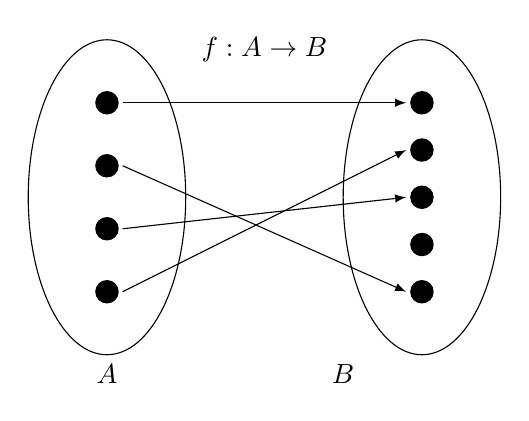
\begin{tikzpicture}[scale=1]
            \foreach \x in {0,...,4}
            {
                \node at (4, -\x*0.6)[circle,fill,inner sep=3pt]{};
            }
            \draw (4,-1.2) ellipse (1 and 2);
    
            \foreach \x in {0,...,3}
            {
                \node at (0, -\x*0.8)[circle,fill,inner sep=3pt]{};
            }
            \draw (0,-1.2) ellipse (1 and 2);
    
            \draw[-latex] (0.2,-0.0) -- (3.8,0.0); 
            \draw[-latex] (0.2,-0.8) -- (3.8,-2.4); 
            \draw[-latex] (0.2,-1.6) -- (3.8,-1.2); 
            \draw[-latex] (0.2,-2.4) -- (3.8,-0.6); 
            
            \node[below] at (0, -3.2){$A$};
            \node[below] at (3, -3.2){$B$};
            \node[above] at (2, 0.4){$f:A \to B$};
        \end{tikzpicture}}
    \end{center}

    \begin{center}
        {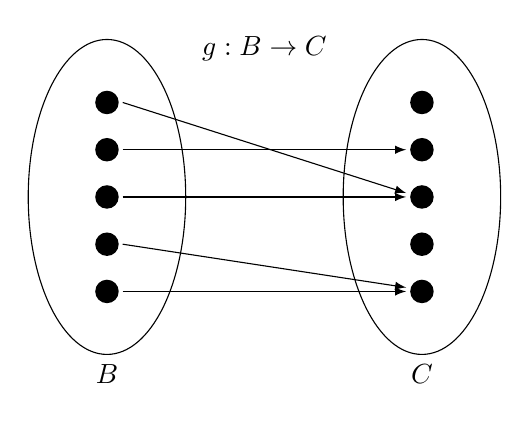
\begin{tikzpicture}[scale=1]
            \foreach \x in  {0,...,4}
            {
                \node at (4, -\x*0.6)[circle,fill,inner sep=3pt]{};
            }
            \draw (4,-1.2) ellipse (1 and 2);
    
            \foreach \x in  {0,...,4}
            {
                \node at (0, -\x*0.6)[circle,fill,inner sep=3pt]{};
            }
            \draw (0,-1.2) ellipse (1 and 2);
    
            \draw[-latex] (0.2,-0.0) -- (3.8,-1.15); 
            \draw[-latex] (0.2,-0.6) -- (3.8,-0.6); 
            \draw[-latex] (0.2,-1.2) -- (3.8,-1.2); 
            \draw[-latex] (0.2,-1.8) -- (3.8,-2.35); 
            \draw[-latex] (0.2,-2.4) -- (3.8,-2.4); 
            
            \node[below] at (0, -3.2){$B$};
            \node[below] at (4, -3.2){$C$};
            \node[above] at (2, 0.4){$g:B \to C$};
        \end{tikzpicture}}
    \end{center}
\end{multicols}

直观感觉,$f$ 就像一张``地图'',为我们提供了从 $A$ 中元素到 $B$ 中元素的特定路线,而 $g$ 则是从 $B$ 中元素到 $C$ 中元素的``地图''。如果我们依次遵循这些``地图'',会发生什么呢?也就是说,让我们把这两张``地图''叠加起来,

\begin{center}
    {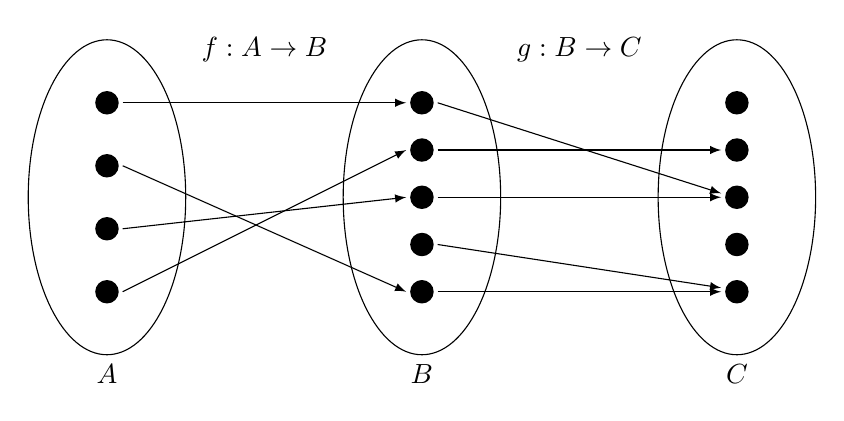
\begin{tikzpicture}[scale=1]
        \foreach \x in {0,...,3}
        {
            \node at (0, -\x*0.8)[circle,fill,inner sep=3pt]{};
        }
        \draw (0,-1.2) ellipse (1 and 2);

        \foreach \x in {0,...,4}
        {
            \node at (4, -\x*0.6)[circle,fill,inner sep=3pt]{};
        }
        \draw (4,-1.2) ellipse (1 and 2);

        \foreach \x in  {0,...,4}
        {
            \node at (8, -\x*0.6)[circle,fill,inner sep=3pt]{};
        }
        \draw (8,-1.2) ellipse (1 and 2);

        \draw[-latex] (0.2,-0.0) -- (3.8,0.0); 
        \draw[-latex] (0.2,-0.8) -- (3.8,-2.4); 
        \draw[-latex] (0.2,-1.6) -- (3.8,-1.2); 
        \draw[-latex] (0.2,-2.4) -- (3.8,-0.6); 

        \draw[-latex] (4.2,-0.0) -- (7.8,-1.15); 
        \draw[-latex] (4.2,-0.6) -- (7.8,-0.6); 
        \draw[-latex] (4.2,-1.2) -- (7.8,-1.2); 
        \draw[-latex] (4.2,-1.8) -- (7.8,-2.35); 
        \draw[-latex] (4.2,-2.4) -- (7.8,-2.4); 
        
        \node[below] at (0, -3.2){$A$};
        \node[below] at (4, -3.2){$B$};
        \node[below] at (8, -3.2){$C$};
        \node[above] at (2, 0.4){$f:A \to B$};
        \node[above] at (6, 0.4){$g:B \to C$};
    \end{tikzpicture}}
\end{center}

然后直接从 $A$ 到 $C$,省略中间环节:

\begin{center}
    {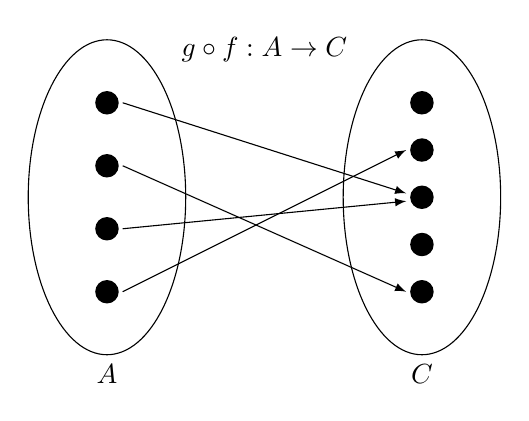
\begin{tikzpicture}[scale=1]
        \foreach \x in {0,...,4}
        {
            \node at (4, -\x*0.6)[circle,fill,inner sep=3pt]{};
        }
        \draw (4,-1.2) ellipse (1 and 2);

        \foreach \x in {0,...,3}
        {
            \node at (0, -\x*0.8)[circle,fill,inner sep=3pt]{};
        }
        \draw (0,-1.2) ellipse (1 and 2);

        \draw[-latex] (0.2,-0.0) -- (3.8,-1.15); 
        \draw[-latex] (0.2,-0.8) -- (3.8,-2.4); 
        \draw[-latex] (0.2,-1.6) -- (3.8,-1.25); 
        \draw[-latex] (0.2,-2.4) -- (3.8,-0.6); 
        
        \node[below] at (0, -3.2){$A$};
        \node[below] at (4, -3.2){$C$};
        \node[above] at (2, 0.4){$g \circ f:A \to C$};
    \end{tikzpicture}}
\end{center}

这看起来是个合理的做法,对吧?当然是的!每当我们有数学对象时,我们总是好奇如何合理地组合、操作和泛化它们。在函数的情况下,我们称这种组合为函数的\textbf{复合}。你可能会注意到,只有当``第一个''函数的值域与``第二个''函数的定义域相同时,这种复合才有意义。这一点在下面的定义中有所体现。

\subsubsection*{定义}

\begin{definition}
    设 $A, B, C$ 为集合,$f : A \to B$ 和 $g : B \to C$ 为函数。考虑函数 $h : A \to C$ 定义为:
    \[\forall a \in A \centerdot h(a) = g(f(a))\]
    我们说 $h$ 是 $g$ 和 $f$ 的\dotuline{复合},写做 $g \circ f$。

    我们也可以将该术语简化为 $f$ 是 ``$g$ 复合 $f$''。
\end{definition}

这结合了我们之前提到的所有概念。要求函数 $f$(``第一个''函数)的值域必须是函数 $g$(``第二个''函数)的定义域。

我们可以将函数直观地理解为一台\emph{机器}或一个\emph{黑箱}。输入定义域中的元素,输出值域中的元素。我们不一定知道机器内部的具体操作,只能看到输出结果。现在,想象将两台机器连接起来,一台执行 $f$,一台执行 $g$;将 $f$ 机器的输出作为 $g$ 机器的输入。最终的输出是集合 $C$ 中的一个元素。我们可以把这两台机器看作是一台更大的机器。这就是\emph{复合} $g \circ f$ 的作用;它相当于一台更大的机器,按特定顺序执行两台机器的操作。

\subsubsection*{符号}

注意符号 $g \circ f$ 的顺序以及它与我们应用函数顺序的对比:先应用 $f$,然后是 $g$,即 $g(f(a))$。用语言描述,我们会将``$g(f(a))$'' 读作 ``$a$ 的 $f$ 的 $g$''。事实上,如果你发现自己难以记住这个顺序,这里有一个建议:将 “$\circ$” 读作 ``在……之后''。因此,$h = g \circ f$ 意味着 ``$g$ 在 $f$ 之后'',因为我们先对 $a$ 元素应用 $f$,然后再应用 $g$。

记住复合函数的符号也很重要,并且要区分函数 $g \circ f$ 本身和将某元素 $x \in A$ 应用于函数 $g \circ f$。例如,要使用 ``$\circ$'' 符号表示``$x$ 的 $f$ 的 $g$'',我们会写
\[(g \circ f)(x)\]
因为我们将函数 $g \circ f$ 应用于元素 $x$。然而,以下符号是\textbf{没有意义的},因为它混淆了函数和元素的概念:
\[g \circ f(x)\]
你能看出区别吗?$f(x)$ 是集合 $B$ 中的一个元素,$B$ 是 $f$ 的值域。但 $g$ 是一个函数。将函数与集合中的元素复合是什么意思?这行不通。通常来说,要注意这一点!当我们必须将多个函数复合在一起时,这种区别尤其重要,例如 $(h \circ (g \circ k) \circ f)(z)$,其中 $z$ 是 $f$ 定义域中的元素,而 $f,g,h,k$ 都是函数。

\subsubsection*{示例}

\begin{example}
    定义函数 $ C : \mathbb{R} \to \mathbb{R}$ 为
    \[\forall x \in \mathbb{R} \centerdot C(x) = x - 273.15\]

    定义函数 $ F : \mathbb{R} \to \mathbb{R}$ 为
    \[\forall x \in \mathbb{R} \centerdot F(x) = \frac{9}{5}x + 32\]

    函数 $C$ 将开尔文温度转换为摄氏温度。

    函数 $F$ 将摄氏温度转换为华氏温度。

    函数 $F \circ C$ 直接将开尔文温度转换为华氏温度。我们可以复合函数的``规则''从而找到直接转换的公式。
    \begin{align*}
        \forall x \in \mathbb{R} \centerdot (F \circ C)(x) &= F(C(x)) = F(x - 273.15) \\
        &= \frac{9}{5} \cdot (x - 273.15) + 32 = \frac{9}{5}-459.67
    \end{align*}
\end{example}

\begin{example}
    设函数 $f : \mathbb{R} \to \mathbb{Z}$ 定义为
    \[\forall x \in \mathbb{R} \centerdot f(x) = \lfloor x \rfloor\]
    ($\lfloor x \rfloor$ 表示 $x$ 向下取整:即满足 $z \le x$ 的\emph{最大}整数 $z \in \mathbb{Z}$。)

    设函数 $g : \mathbb{Z} \to \mathbb{N}$ 定义为
    \[\forall z \in \mathbb{Z} \centerdot g(z) = \begin{cases}
        -z & \text{如果}\;z<0 \\
        z+1 & \text{如果}\;z \ge 0
    \end{cases}\]

    我们来找出 $g \circ f$。

    注意,只要 $x \in \mathbb{R} < 0$,我们都可以得到 $\lfloor x \rfloor < 0$。同理,只要 $x \in \mathbb{R} \ge 0$,我们都可以得到 $\lfloor x \rfloor \ge 0$。这告诉我们 $g \circ f$ 是一个\textbf{分段}函数:
    \[\forall x \in \mathbb{R} \centerdot (g \circ f)(x) = \begin{cases}
        -\lfloor x \rfloor & \text{如果}\;z<0 \\
        \lfloor x \rfloor+1 & \text{如果}\;z \ge 0
    \end{cases}\]
    问题:这个函数是单射吗?是满射吗?试着证明你的结论。
\end{example}

\begin{example}
    定义函数 $f : \mathbb{N} \to \mathbb{N}, g : \mathbb{Z} \to \mathbb{N}, h : \mathbb{Z} \to \mathbb{N}$ 为:
    \begin{align*}
        \forall n \in \mathbb{N} \centerdot f(n) &= n + 3 \\
        \forall n \in \mathbb{N} \centerdot g(n) &= n^2 \\
        \forall n \in \mathbb{N} \centerdot h(n) &= 2n - 1
    \end{align*}
    (问题:你确定这些函数都是良好定义的吗?为什么?)

    我们可以找到 $g \circ f$ 和 $h \circ g$ 的``规则'':
    \begin{align*}
        \forall n \in \mathbb{N} \centerdot (g \circ f)(n) &= g(f(n)) = g(n + 3) = (n + 3)^2 = n^2 + 6n + 9 \\
        \forall n \in \mathbb{N} \centerdot (h \circ g)(n) &= h(g(n)) = h(n^2) = 2n^2-1
    \end{align*}

    我们可以由此得到进一步复合的规则,比如 $h \circ (g \circ f)$:
    \begin{align*}
        \forall n \in \mathbb{N} \centerdot \big(h \circ (g \circ f)\big)(n) &= h\big((g \circ f)(n)\big) = h(n^2 + 6n + 9) \\
        &= 2(n^2 + 6n + 9) - 1 \\
        &= 2n^2 + 12n + 17
    \end{align*}

    类似地,我们可以找到 $(h \circ g) \circ f$ 的规则:
    \begin{align*}
        \forall n \in \mathbb{N} \centerdot \big((h \circ g) \circ f\big)(n) &= (h \circ g)(f(n)) = (h \circ g)(n + 3) \\
        &= 2(n + 3)^2 - 1 = 2(n^2 + 6n + 9) - 1 \\
        &= 2n^2 + 12n + 17
    \end{align*}
\end{example}

看一下上面两个结果,他们是相等的!也就是说,从\emph{函数}意义上讲,我们刚刚通过证明在\emph{每一个}允许的输入上都能产生相同的输出,从而\emph{证明}了
\[h \circ (g \circ f) = (h \circ g) \circ f\]

\subsubsection*{复合结合律}

在前面的例子中,函数 $f, g, h$ 并没有什么特别之处。实际上,我们得到的结果在\emph{一般情况下}都是成立的。下面的定理和证明将表明这一点。我们要证明的是函数复合满足\textbf{结合律}。这意味着在进行多重函数复合时,可以随意移动括号,而不影响结果。

\begin{theorem}
    设 $A,B,C D$ 为任意集合。设 $f : A \to B, g : B \to C, h : C \to D$ 为函数。则
    \[h \circ (g \circ f) = (h \circ g) \circ f\]
\end{theorem}

\begin{proof}
    我们要证明对于任意可能的输入,函数 $(h \circ g) \circ f$ 和函数 $h \circ (g \circ f)$ 的输出相同。

    给定 $x \in A$,应用\emph{复合}的定义,可得
    \[[h \circ (g \circ f)](x) = h\big((g \circ f)(x)\big) = h\big(g(f(x))\big)\]
    且
    \[[(h \circ g) \circ f](x) = \big(h \circ g\big)(f(x)) = h\big(g(f(x))\big)\]
\end{proof}

\subsubsection*{复合与映射}

现在有一个有趣的问题:如果我们将两个具有相同性质的函数复合起来,会发生什么?这个性质依然存在吗?比如,如果我们复合两个单射函数,结果还是单射函数吗?是否只需要其中一个函数是单射,就能确保复合后的函数也是单射?

同理,假设我们有两个函数的复合。如果已知复合后的函数是满射,我们能否确定其中一个函数也是满射?还是说两个函数都必须是满射?

在这部分内容中,我们将陈述并证明一些关于这些问题的结论。我们也会让你在本节和本章末尾的练习中证明一些相关的事实,或者找到适当的反例。

\begin{proposition}
    设 $A, B, C$ 为集合,$f : A \to B$ 和 $g : B \to C$ 为函数。如果 $g \circ f$ 为单射,则 $f$ 必为单射。
\end{proposition}

(请注意,这里并不假设 $g$ 具有任何特定性质;$g$ 甚至不一定是单射!作为练习,试着找出函数 $f: A \to B$ 和 $g: B \to C$ 的两个例子:一个例子中 $g \circ f$ 是单射且 $g$ 也是单射,另一个例子中 $g \circ f$ 是单射但 $g$ 不是单射。)

\begin{proof}
    给定 $x,y \in A$,假设 $f(x)=f(y)$,我们要证明 $x=y$。

    因为 $g$ 是良好定义的函数,所以 $g(f(x)) = g(f(y))$。

    这意味着 $(g \circ f)(x) = (g \circ f)(x)$。

    因为 $g \circ f$ 为单射,所以 $x=y$。这正是我们要证明的。
\end{proof}

事实证明,我们刚刚证明的命题它的\emph{逆命题}并不成立。因为这个命题涉及所有函数,所以要证伪它,我们需要提供一个反例。

\begin{proposition}
    设 $A, B, C$ 为集合,$f : A \to B$ 和 $g : B \to C$ 为函数。假设 $f$ 为单射,则 $g \circ f$ 不一定为单射。
\end{proposition}

在阅读我们的反例之前,试着自己动手想一个反例。记住,你不需要找到最有趣或最复杂的反例,也不一定要有明确的规则;只要能定义出一个反例即可!

\begin{proof}
    我们将构造一个反例。

    定义 $A = \{1, 2\}, B = \{\heartsuit, \diamondsuit\}, C = \{\bigstar\}$。

    定义函数 $f$ 为 $f(1) = \heartsuit, f(2) = \diamondsuit$。

    易得 $f$ 为单射,因为 $f(1) \ne f(2)$。

    定义函数 $g$ 为 $g(1) = g(2) = \bigstar$ 。

    则 $g \circ f$ 定义为 $(g \circ f)(1) = \bigstar, (g \circ f)(2) = \bigstar$。
    
    这表明 $g \circ f$ 不是单射,因为 $(g \circ f)(1) = (g \circ f)(2)$,而 $1 \ne 2$。
\end{proof}

% !TeX root = ../../../book.tex

\subsection{反函数}

\subsubsection*{引言}

此前我们提到,\textbf{双射}函数 $f: A \to B$ 具有一个重要性质:它能在集合 $A$ 和 $B$ 的元素之间建立``一一对应''关系。对于任意 $a \in A$,\emph{有且只有}一个 $b \in B$ 满足 $f(a) = b$,此乃良好定义的函数的要求;同时,由于 $f$ 是双射,$a$ 也是\emph{唯一一个}与 $b$ 关联的元素。基于这种双向唯一性,我们可以``逆转'' $f$。也就是说,给定任意 $b \in B$,存在唯一一个 $a \in A$ 使得 $f(a) = b$,这就是\textbf{反函数}。本节将通过\emph{函数复合}和\emph{恒等函数}形式化这一概念。这也说明双射关系存在于两个集合之间,而非单向;一旦获得一个方向的双射,必然存在反向的双射。

在正式定义之前,我们简要回顾一下\textbf{恒等函数}的定义,它在反函数的定义中扮演至关重要的角色。
\begin{center}
    给定集合 $X$,\textbf{恒等函数} $\id_X: X \to X$ 定义为 $\forall z \in X \centerdot \id_X(z) = z$。
\end{center}

\subsubsection*{定义}

请注意,以下定义未预设函数为双射,仅形式化反函数的含义。反函数与双射的关系将在后续证明。

\begin{definition}
    设 $f:A \to B$ 为函数。若存在函数 $g:B \to A$ 使得 
    \[g \circ f : A \to A \text{\ 满足\ } g \circ f = \id_A\] 
    \[f \circ g : B \to B \text{\ 满足\ } f \circ g = \id_B\]
    则称 $g$ 是 $f$ 的\dotuline{反函数},记作 $g = f^{-1}$。
\end{definition}

(请注意,上述定义中的假设和结论隐含 $B = \im_f(A)$ 以确保 $g$ 是良好定义的函数;同理,$A = \im_g(B)$。)

\subsubsection*{示例}

回顾此前讨论双射时涉及的函数。通过练习,我们已经证明该函数是双射,下面将求其反函数。

\begin{example}
    定义函数 $h : \mathbb{R} - \{-1\} \to \mathbb{R}- \{1\}$ 为
    \[\forall x \in \mathbb{R} - \{-1\} \centerdot h(x) = \frac{x}{1+x}\]

    为了找到 $h$ 的候选反函数,通常可以将 $h$ 的``规则''等同于一个新变量,然后求解 $x$。

    这里,我们令 $h(x) = y$。那么我们如何``逆转''这个过程,并用 $y$ 表示 $x$ 呢?我们可以通过以下代数步骤来实现:
    \begin{align*}
        h(x) = y &\iff \frac{x}{1+x} = y \\
        &\iff (1 + x)y = x \\
        &\iff xy + y = x \\
        &\iff y = x(1 - y) \\
        &\iff x = \frac{y}{1-y}
    \end{align*}

    上述推导得到 $h$ 的候选反函数。需注意:此过程并非严格证明。为了严谨表述,我们定义新函数 $H$ 并证明 $H = h^{-1}$。若直接使用 $h^{-1}$ 将导致循环论证,因为反函数存在性尚待证明,不能在证明开始时就假定反函数存在。

    \begin{proof}
        为了简便,我们定义 $S = \mathbb{R} - \{-1\}, T = \mathbb{R}- \{1\}$,则 $h:S \to T$。

        设函数 $H: T \to S$ 定义为 $\forall y \in T \centerdot H(y) = \frac{y}{1-y}$。

        首先,证明 $H$ 是良好定义的函数。对于每个 $y \in T$,都有 $y \ne 1$,所以 $1-y \ne 0$。因此分数 $\frac{y}{1-y}$ 是良好定义的实数。

        此外,还可以推导出 $\frac{y}{1-y} \ne -1$。为了引出矛盾而假设 $\frac{y}{1-y} = -1$,等式两边同时乘以 $1-y$ 得 $y = y-1$,这显然是矛盾的。\\

        接着,证明 $H \circ h = \id_S$。给定 $x \in S$,可得
        \begin{align*}
            (H \circ h)(x) &= H(h(x)) = H\Big(\frac{x}{1+x}\Big) \\
            &=\frac{\frac{x}{1+x}}{1-\frac{x}{1+x}} \cdot \frac{1+x}{1+x} = \frac{x}{(1+x)-x} \\
            &=\frac{x}{1} = x\\
        \end{align*}

        最后,证明 $h \circ H = \id_T$。给定 $y \in T$,可得
        \begin{align*}
            (h \circ H)(y) &= h(H(y)) = h\Big(\frac{y}{1-y}\Big) \\
            &=\frac{\frac{y}{1-y}}{1+\frac{y}{1-y}} \cdot \frac{1-y}{1-y} = \frac{y}{(1+y)-y} \\
            &=\frac{y}{1} = y
        \end{align*}

        综上,根据反函数的定义,$H = h^{-1}$。
    \end{proof}
\end{example}

\subsubsection*{双向检查}

若称函数 $f: A \to B$ 存在反函数 $g: B \to A$,则\textbf{关键}在于必须证明两个复合函数均等于恒等函数;也就是说,必须证明
\[f \circ g = \id_B \quad \text{且} \quad g \circ f = \id_A\]

初学者可能会忽略此验证,或不解其必要性。为了加深理解,\ref{sec:section7.5.4} 节的练习 \ref{exc:exercises7.5.2} 要求构造一个反例,其中``一个方向''的复合可得恒等函数,但``另一方向''的复合却无法得到恒等函数,此时函数并非真正意义上的\emph{反函数}。建议尝试构造多个此种类型的实例,以深刻理解双向验证的重要性。

% !TeX root = ../../../book.tex

\subsection{双射 $\iff$ 可逆}

正如我们一直暗示的,双射函数必然存在逆函数。该命题的逆命题同样成立,因此我们可以完整陈述并证明这一``\emph{当且仅当}''命题。章节标题中的``\textbf{可逆}''通常指``具有反函数''。

\begin{theorem}
    设 $A, B$ 为任意集合。$f : A \to B$ 为函数。则
    \[f \text{\ 为双射} \iff f \textbf{\ 存在反函数\ } f^{-1}: B \to A\]
\end{theorem}

\begin{proof}
    ($\implies$) 假设 $f$ 为双射。这意味着 $f$ 即是单射又是满射。我们按如下规则定义 $f$ 的反函数 $g : B \to A$: 

    给定 $b \in B$。由 $f$ 是满射可知 
    \[\exists a \in A \centerdot f(a)=b\]

    给定这样的 $a$。由 $f$ 是单射可知
    \[\forall x \in A \centerdot x \ne a \implies f(x) \ne f(a) = b\]

    这表明 $a$ 是 $A$ 中\emph{唯一}满足 $f(a) = b$ 的元素。定义 $f(b) = a$,这是一个良好定义的函数。

    易得 $(f \circ g)(b) = f(g(b)) = f(a) = b$,所以 $f \circ g = \id_B$。

    并且 $(g \circ f)(a) = g(f(a)) = g(b) = a$,所以 $g \circ f = \id_A$。

    因此,$g = f^{-1}$,即 $f$ 可逆。\\

    ($\impliedby$) 假设 $f$ 有反函数 $f^{-1} : B \to A$。

    首先,证明 $f$ 为单射。给定 $a_1, a_2 \in A$,易得
    \begin{align*}
        f(a1) = f(a2) &\implies f^{-1}(f(a_1)) = f^{-1}(f(a_2)) & f^{-1}: B \to A \text{\ 为函数} \\
        &\implies (f^{-1} \circ f)(a_1) = (f^{-1} \circ f)(a_2) & \text{复合的定义} \\
        &\implies \id_A(a_1) = \id_A(a_2) & \textbf{恒等函数的定义} \\
        &\implies a_1 = a_2 & \textbf{恒等函数的定义} 
    \end{align*}

    因此 $f$ 为单射。

    接着,证明 $f$ 为满射。给定 $b \in B$。因为 $f^{-1}$ 为函数,因此 $\exists a \in A \centerdot f^{-1}(b)=a$。给定这样的 $a$,易得
    \begin{align*}
        f^{-1}(b) = a &\implies f(f^{-1}(b)) = f(a) & f : A \to B \text{\ 为函数} \\
        &\implies (f \circ f^{-1})(b) = f(a) & \text{复合的定义} \\
        &\implies \id_B(b) = f(a) & \textbf{恒等函数的定义} \\
        &\implies b = f(a) d& \textbf{恒等函数的定义} 
    \end{align*}

    因此 $f$ 为满射。
\end{proof}

\subsubsection*{证明函数为双射}

该定理提供了一种证明函数 $f : A \to B$ 为双射的新方法:无需分别证明 $f$ 是单射和满射,只需定义函数 $g : B \to A$ 并证明 $g$ 是 $f$ 的\textbf{反函数}(即 $g = f^{-1}$)。根据定理,即可推出 $f$ 为双射。在实际应用中,可以根据具体情况选择更便捷或更熟悉的策略。这两种方法均可行!

\subsubsection*{反函数的反函数}

以下推论直接源于上述定理。我们称之为推论而非新定理,是因为其结论未引入新内容——如证明所示,其本质是对原定理的应用。

\begin{corollary}
    设 $A, B$ 为任意集合。$f : A \to B$ 为函数。

    若 $f$ 为双射,则 $f^{-1}$ 存在且亦为双射。

    此外 $\big(f^{-1}\big)^{-1} = f$。
\end{corollary}

\begin{proof}
    假设 $f$ 有反函数 $f^{-1} : B \to A$。根据反函数的定义,这意味着 $f \circ f^{-1} = \id_B$ 且 $f^{-1} \circ f = \id_A$。

    再次通过反函数的定义,这些条件证明了 $(f^{-1})^{-1}=f$!这表明 $f^{-1}$ 有一个反函数(即 $f$ 本身),因此根据上面的定理可得 $f^{-1}$ 必为双射。
\end{proof}

\subsubsection*{复合函数的反函数}

在进入练习和下一节之前,让我们总结一下本章的核心内容。我们将在此陈述两个重要结论,其证明留作本章练习。完成这些证明将帮助你:
\begin{enumerate}[label=(\alph*)]
    \item 巩固对已有概念的理解,包括函数、映射、复合、反函数等;
    \item 获得关于如何定义复合函数的反函数的重要结论。
\end{enumerate}

\begin{proposition}
    设函数 $f : A \to B$ 和 $g : B \to C$ 为双射。定义复合函数 $h : A \to C$ 为 $h = g \circ f$。
    
    则 $h$ 也为双射。
\end{proposition}

\begin{proof}
    留作练习 \ref{exc:exercises7.8.9}。
\end{proof}

\begin{proposition}
    设函数 $f : A \to B$ 和 $g : B \to C$ 为双射。定义复合函数 $h : A \to C$ 为 $h = g \circ f$。
    
    则 $h$ 可逆,且 $h^{-1} = f^{-1} \circ g^{-1}$。
\end{proposition}

\begin{proof}
    留作练习 \ref{exc:exercises7.8.10}。
\end{proof}

% !TeX root = ../../../book.tex

\subsection{习题}\label{sec:section7.5.4}

\subsubsection*{温故知新}

以口头或书面的形式简要回答以下问题。这些问题全都基于你刚刚阅读的内容,所以如果忘记了具体的定义、概念或示例,可以回去重读相关部分。确保在继续学习之前能够自信地回答这些问题,这将有助于你的理解和记忆!

\begin{enumerate}[label=(\arabic*)]
    \item 函数复合运算满足结合律吗?(也就是说,括号的顺序是否重要?)为什么满足或者为什么不满足?
    \item 函数复合运算满足交换律吗?(也就是说,我们可以颠倒顺序进行运算吗?)为什么满足或者为什么不满足?
    \item 假设 $f : A \to B$ 和 $g : B \to A$ 为函数。我们如何证明 $g = f^{-1}$?
    \item 假设 $f : A \to B$ 为双射。它的反函数也是双射吗?
\end{enumerate}

\subsubsection*{小试牛刀}

尝试回答以下问题。这些题目要求你实际动笔写下答案,或(对朋友/同学)口头陈述答案。目的是帮助你练习使用新的概念、定义和符号。题目都比较简单,确保能够解决这些问题将对你大有帮助!

\begin{enumerate}[label=(\arabic*)]
    \item 设 $O$ 为奇数集,设 $E$ 为偶数集。定义\textbf{双射}函数 $f : O \to E$,并通过找到它的反函数证明 $f$ 确实为双射。
    \item 在这个问题中,我们希望你能通过一个例子来展示,当我们尝试找到一个函数的反函数时,验证两个复合函数\textbf{都能}得到恒等函数是多么重要。\\
    定义集合 $A, B$ 以及函数 $f : A \to B, g : B \to A$ 使得
    \[\forall x \in A \centerdot g(f(x)) = x\]
    但
    \[\exists y \in B \centerdot f(g(y)) \ne y\]
    (\textbf{建议}:你可以找一个例子,其中 $A$ 和 $B$ 都只有一到两个元素……或者,你可以找一个例子,其中 $A=B=\mathbb{N}$。)
    \item 设 $U = \{y \in \mathbb{R} \mid -1 < y < 1\}, I = \{y \in \mathbb{R} \mid -6 < y < 12\}$。\\
        设函数 $g : U \to I$ 定义为 $\forall x \in U \centerdot g(x) = 9x + 3$。
        证明 $g$ 是双射,并找到 $g^{-1}$。
    \item 定义函数 $f : \mathbb{Z} \to \mathbb{N}$ 为
    \[\forall z \in \mathbb{Z} \centerdot f(z) = \begin{cases}
        -2z + 2 & \text{如果}\; z \le 0 \\
        2z-1 & \text{如果}\; z > 0
    \end{cases}\]
    证明 $f$ 是双射,并找到 $f^-1$。\\
    (\textbf{提示}:你给出的反函数也是分段定义的。在你的证明中要小心处理可能出现的各种情况。)
    \item \textbf{挑战性问题}:定义 $I = \{y \in \mathbb{R} \mid -1 < y < 1\}$。找到函数 $f : I \to \mathbb{R}$ 是双射函数,并证明之。\\
    (\textbf{提示}:无需使用任何三角函数。可以考虑在表达式中使用 $|x|$……)
\end{enumerate}


\newpage
% !TeX root = ../../book.tex
\section{基数}

% !TeX root = ../../../book.tex

\subsection{引言与定义}

我们如此关心双射的一个重要原因是,它们可以帮助我们比较\textbf{集合的大小}。你可能对此已有直觉认识:例如,集合
\[\{1, 2, 3, 4, 5\}\]
显然包含 $5$ 个元素,它是一个\textbf{有限集}。而集合
\[\mathbb{N} = \{1, 2, 3, 4, 5, \dots \}\]
则是\textbf{无限集}。我们知道 $\mathbb{Z}$, $\mathbb{Q}$ 和 $\mathbb{R}$ 也是都无限集。那么,这些集合的大小究竟是多少?我们能够比较它们的大小吗?我们如何\emph{在数学上}进行比较?\emph{无限集}到底意味着什么?是否存在``不同大小的无穷大''?

\subsubsection*{双射``配对''元素}

假设桌上有 $5$ 支笔和 $5$ 本书,但我们不知道如何计数。如何在不依赖数字的情况下验证笔和书的数量相同?显然不能直接说``两者都是 $5$'',此时\emph{双射}就派上了用场。我们可以将每支笔与每本书\emph{一一配对}。通过排列物品并建立对应关系,本质上是在笔的集合与书的集合之间构造双射。这一思想极其重要:
\begin{center}
    \large{在基数的国度里,双射为王。}
\end{center}

想象我们对基数的研究是一段穿越基数王国的旅程。在此领域中,我们臣服于双射王——因为他统治着一切。唯有他能判定两个集合是否具有\emph{相同的基数},无论是有限集还是无限集。

此外,我们\emph{必须}采用集合论语言,因为后续结论可能出人意料甚至令人震惊!严谨的定义和概念能确保推演的精确性。尽管某些结论可能反直觉,但将它们建立在既有概念和已证定理之上,方能获得在数学上真正令人信服的结论!

\clearpage

\subsubsection*{定义与符号}

首先,我们定义什么是\textbf{有限集}。

\begin{definition}
    设 $S$ 为任意集合。称 $S$ 是\dotuline{有限集} 当且仅当
    \[\exists n \in \mathbb{N} \cup \{0\} \text{\ 使得存在双射\ } f : S \to [n]\]
    在这种情况下,我们用 $|S| = n$ 表示 $S$ 的\dotuline{大小}为 $n$。
\end{definition}

注意:空集 $S = \varnothing$ 是有限集,因为 $[0] = \varnothing$。这就是为什么我们在定义中取 $n \in \mathbb{N} \cup \{0\}$,而不仅仅是 $n \in \mathbb{N}$。函数 $f : \varnothing \to \varnothing$ 是一个双射,它实际上是一个\emph{空关系}。(请记住,函数是一种关系!)

根据定义,形如 $[n]$ 的集合是有限集。它们是标准的有限集实例,大小为 $|[n]| = n$。因此,要证明一个集合 $S$ 的大小为 $n$,需要构造 $S$ 和 $[n]$ 之间的双射。例如,考虑集合 $\{1, 3, 5\}$。显然,它的大小为 $3$。我们可以通过构造双射 $f : \{1, 3, 5\} \to [3]$ 来证明这一点,该双射定义为 $f(1) = 1, f(3) = 2, f(5) = 3$。

思考一下有限集是否可以有两个\emph{不同的}大小?这是一个有趣问题。尽管定义未明确排除这种可能性,但可以\emph{证明}有限集的大小是唯一的。想一想如何证明这一点……我们将在完成基本定义之后给出证明。

\begin{definition}
    设 $S$ 为任意集合。称 $S$ 是\dotuline{无限集} 当且仅当 $S$ 不是有限集。

    也就是说,若 $\forall n \in \mathbb{N} \cup \{0\}$,所有可能的函数 $f : S \to [n]$ 都不是双射,则 $S$ 是无限集。

    当 $S$ 为无限集时,我们用 $|S|$ 表示集合的\dotuline{基数 (Cardinality)}。
\end{definition}

将无限集定义为``非有限集''可能有些奇怪,但它确实反映了这两个概念之间的直观对立。一个集合不可能既是有限集又是无限集,因此通常选择定义其中一个,而将另一个定义为``其他所有情况''。

此外,我们\textbf{不会}用 $|S| = \infty$ 来表示集合是无限的。正如后续将看到的,实际上\textbf{存在许多不同``级别''的无限集}。虽然这听起来可能非常奇特,但你会理解其中含义。没错,无限集也有不同的``大小'',我们将用 $|S|$ 表示集合 $S$ 的\textbf{基数},以便比较集合的大小。若写成 $|S| = \infty$,则暗示只有``一种无限'',这是错误的。

接下来,我们将主要区分两种\emph{类型}的无限集,并展示关于常见集合(如 $\mathbb{N}, \mathbb{Z}, \mathbb{Q}, \mathbb{R}$)的有趣结论。以下定义将解释这两种类型。

\begin{definition}
    设 $S$ 为任意集合。

    称 $S$ 为\dotuline{可数无限集},当且仅当存在双射 $f : S \to \mathbb{N}$。

    称 $S$ 为\dotuline{不可数无限集}(或\dotuline{不可数的}),当且仅当 $S$ 是无限集且每个函数 $f : S \to \mathbb{N}$ 都不是双射。
\end{definition}

给定无限集 $S$,可以根据其基数 $|S|$ 与 $|\mathbb{N}|$ 的关系分为两类。称之为\textbf{可数无限}体现了 $\mathbb{N}$ 的直观特性:$\mathbb{N}$ 的元素``无穷无尽'',但我们可以尝试枚举它们。它具有第一个元素、第二个元素、第三个元素……尽管无法在有限时间内枚举全部,但可以设想一个不朽的神奇机器人逐个输出它们。无论指定哪个自然数,机器人\emph{最终}都会将其打印出来。

但并非所有无限集都能这样处理。这便是\textbf{不可数无限}的概念。这类集合是无限的,但却没有与 $[n]$ 形式集合的双射关系,它``如此之大''以至于无法定义``第一元素''、``第二元素''、``第三个元素''等等。存在\textbf{双射} $f : S \to \mathbb{N}$ 意味着可以标记 $S$ 的所有元素,实现与自然数的配对。若无法做到,则集合不可数。你可能质疑此类集合的存在!不必担心,我们将展示实例。现在只需理解\textbf{可数无限}与\textbf{不可数无限}的区别:关键在于是否存在到 $\mathbb{N}$ 的\textbf{双射}。

\subsubsection*{基数比较}

正如我们之前提到的,当集合 $S$ 为无限集时,我们使用 $|S|$ 来\textbf{比较} $S$ 与其他集合的基数。我们不会写作 $|S| = \infty$,而是写作 $|S| = |T|$ 表示 $S$ 与 $T$ 具有\emph{相同的}基数(无论具体数值如何),或写作 $|S| < |P|$ 表示集合 $P$ 的基数\emph{严格大于} $S$。以下定义通过函数(特别是不同类型的映射)阐述基数比较的方式:

\begin{definition}
    设 $S, T$ 为任意集合。

    \begin{itemize}
        \item 记 $|S|=|T|$,当且仅当存在\textbf{双射} $ f : S \to T$。\\
            此时称 $S$ 和 $T$ 具有\textbf{相同的基数}。
        \item 记 $|S|\le|T|$ 当且仅当存在\textbf{单射} $ f : S \to T$。\\
            此时称 $S$ 的基数\textbf{至多}为 $|T|$。
        \item 记 $|S|<|T|$ 当且仅当 $|S|\le|T|$ 且 $|S|\ne|T|$。\\
            此时称 $S$ 的基数\textbf{严格小于} $T$ 的基数。
        \item 记 $|S|\ge|T|$ 当且仅当存在\textbf{满射} $ f : S \to T$。\\
            此时称 $S$ 的基数\textbf{至少}为 $|T|$。
        \item 记 $|S|>|T|$ 当且仅当 $|S|\ge|T|$ 且 $|S|\ne|T|$。\\
            此时称 $S$ 的基数\textbf{严格大于} $T$ 的基数。
    \end{itemize}
\end{definition}

我们可以用两种不同的方式来解释这些定义背后的内涵:

一般来说,$f : A \to B$ 是单射表示 $|A| \le |B|$,而 $g : A \to B$ 是满射表示 $|A| \ge |B|$。可以通过示意图理解该定义:$A \to B$ 存在单射意味着能将 $A$ 的元素唯一配对到 $B$ 的元素(无重叠),但 $B$ 中可能有剩余元素;$A \to B$ 存在满射则意味着能用 $A$ 的元素覆盖 $B$ 的所有元素(可能有重叠),因此 $A$ 的元素可能更多。当这两种情况同时成立(即存在 $A$ 到 $B$ 的双射)时,表明 $A$ 和 $B$ 具有相同的基数——所有元素都能一一配对。这是一个直观的解释,旨在阐明定义的内涵,并非严格证明。但基于这些定义,我们就能证明或证伪相关命题!要比较集合的基数——即使是无限集——只需找到具有特定性质的函数。本章建立的方法将在探索基数王国的旅程中发挥重要作用。

另一种理解方式是:``具有相同基数''可视为``所有集合的集合''上的``等价关系''。这里需要为这些短语加引号,因为根据 \ref{sec:section3.3.5} 节罗素悖论的阐述,不存在``所有集合的集合''。因此在严格数学意义上,讨论该``集合''上的等价关系没有意义。但从不严谨的直观角度看,其性质如下:

\begin{itemize}
    \item 给定任意集合 $S$,它当然跟其自身存在双射,即恒等函数 $\id_S : S \to S$。这表明 $|S|=|S|$,即``具有相同基数''关系具有``自反性''。
    \item 假设 $|S| = |T|$,则存在双射 $f:S \to T$。是否也存在双射 $g : T \to S$ 呢?当然存在!我们可以令 $g=f^{-1}$,显然 $g$ 也是双射。这表明 $|T| = |S|$,即``具有相同基数''关系具有``对称性''。
    \item 假设 $|S| = |T| = |U|$,则存在双射 $f : S \to T$ 和 $g : T \to U$。是否也存在双射 $h : S \to U$ 呢?当然存在!因为复合 $g \circ h$ 也是双射(此前练习已证明)。这表明 $|S| = |U|$,即``具有相同基数''关系具有``传递性''。
\end{itemize}

再次强调,这并非\emph{完全严谨}的表述,但有助于理解抽象概念。我们正在建立一种通过函数比较任意两个集合基数的方法,所有集合将按其基数归类。令人惊讶的是,我们即将证明:\emph{基数的种类是可数无穷多的}。

\subsubsection*{康托尔定理}

以下结论和证明源于十九世纪中后期德国数学家乔治·康托尔 (Georg Cantor) 的研究。如今,数学家们已普遍接受这一结论及其深远影响。然而在当时,该观点极具争议性,以至于部分数学家拒绝承认。康托尔的工作和思想最终推动了形式集合论的发展。

说明其命此结论的证明被称为\textbf{康托尔对角线论证}。后文将展示类似论证,并解释为什么它以``对角线''命名。眼下,我们更关注定理本身。

\begin{theorem}
    设 $S$ 为任意集合。则 $|S| < |\mathcal{P}(S)|$。
\end{theorem}

该定理表明:\textbf{任意集合幂集的基数总是严格大于其本身的基数}。对有限集而言这是显然的——已知 $[n]$ 的幂集元素数为 $2^n$,即 $|\mathcal{P}([n])| = 2^n$(练习 \ref{exc:exercises7.8.30} 将要求利用基数的相关结论通过归纳法证明此结论)。显然 $n < 2^n$ 对所有 $n \in \mathbb{N}$ 均成立。而定理进一步指出:该关系对\textbf{无限集}同样成立。这意味着存在一条无限集的链条,每一个集合都比前一个更大。通过不断取前一个集合的幂集可得:
\[|\mathbb{N}| < |\mathcal{P}(\mathbb{N})| < \big|\mathcal{P}\big(\mathcal{P}(\mathbb{N})\big)\big| < \Big|\mathcal{P}\Big(\mathcal{P}\big(\mathcal{P}(\mathbb{N})\big)\Big)\Big| < \dots
\]
接下来我们来证明该定理。此证明过程简洁而精妙,因此无需纠结论证的构造,只需理解其逻辑脉络。

\begin{proof}
    设 $S$ 为任意集合。为了引出矛盾而假设 $|S| \ge |\mathcal{P}(S)|$。

    这意味着存在满射函数 $g : S \to \mathcal{P}(S)$。

    定义 $T = \{X \in S \mid X \notin g(X)\}$。(这是合理的,因为对于任意 $X \in S, g(X) \in \mathcal{P}(S)$,都有 $g(X) \subseteq S$。因此,要么 $X \in g(x)$ 要么 $X \notin g(x)$。)

    根据集合构建符的定义可得 $T \subseteq S$。这意味着 $T \in \mathcal{P}(S)$。

    因为 $g$ 为满射,所以 $\exists Y \in S$ 使得 $g(Y) = T$。给定这样的 $Y$。

    此时,$Y \in T$ 是否成立?考虑如下两种情形:
    \begin{itemize}
        \item 若 $Y \in T$,则根据 $T$ 的定义可得 $Y \notin g(Y)$。然而,$g(Y) = T$,这意味着 $Y \notin T$。这与假设矛盾。$\hashx$
        \item 若 $Y \notin T$,则根据 $T$ 的定义可得 $Y \in g(Y)$。然而,$g(Y) = T$,这意味着 $Y \in T$。这与假设矛盾。$\hashx$
    \end{itemize}
    
    无论上述哪种情形,都会推出矛盾。$\hashx$

    因此不存在从 $S$ 到 $\mathcal{P}(S)$ 的满射,即 $|S| < |\mathcal{P}(S)|$。
\end{proof}

回顾 \ref{sec:section7.4.5} 节的练习 \ref{exc:exercises7.4.4}。请注意,我们要求你定义一个从 $\mathbb{N}$ 到 $\mathcal{P}(\mathbb{N})$ 的函数,并证明它不是满射。我们无需知道你定义的函数具体是什么!因为我们知道相关定理,因此确定你不可能定义一个满射!

\subsubsection*{讨论:公理与定义}

必须承认一点:我们略过了一些关于\emph{定义}和\emph{定理}的细节。定理是需要从基本假设中证明的结论。根据\emph{定义}(至少在本书的语境下),一个从 $A$ 到 $B$ 的双射(即同时为单射和满射)足以证明 $|A| = |B|$。类似地,若存在从 $A$ 到 $B$ 的单射和从 $B$ 到 $A$ 的单射,也足以保证 $|A| = |B|$,从而 $A$ 和 $B$ 之间必然存在双射。

尽管这些结论看似合理,但并\emph{并非显而易见}。假设我们有一个从 $A$ 到 $B$ 的单射函数和一个从 $B$ 到 $A$ 的单射函数,这能否保证两个集合间存在双射?我们期望如此,但这不能作为证明。实际上,该结论被称为\textbf{康托尔-施罗德-伯恩斯坦 (Cantor-Schroeder-Bernstein) 定理}:

\begin{theorem}[康托尔-施罗德-伯恩斯坦定理]
    设 $A,B$ 为任意集合,$f : A \to B$ 和 $g : B \to A$ 为单射,则存在双射 $h : A \to B$。
\end{theorem}

没错,这是一个\emph{定理},且证明并不简单!事实上,该定理存在一种\emph{构造性}证明:它提供了一种算法,利用两个单射 $f : A \to B$ 和 $g : B \to A$ 来构造双射 $h : A \to B$。鉴于本书的目标以及时间和空间的限制,我们无需单独展开此定理,更不必讨论其构造性证明。将单射和满射在基数比较中的作用视为定义即可;这些结论看起来很直观,我们可以直接接受它们。但需注意,我们是基于严格的数学基础来接受此结论的。若你对细节及其影响感兴趣,可以考虑选修一门关于\textbf{集合论}的课程或阅读一本关于\textbf{集合论}的书。

本质上,核心问题在于我们预设了\emph{任意}两个集合 $A$ 和 $B$ 的基数可进行有意义的\emph{比较},即对于任意 $A$ 和 $B$,我们假设能断言 $|A| \le |B|$ 或 $|B| \le |A|$(或两者相等)。然而,如何\emph{保证}这种比较对所有集合成立?这并非简单问题!本书中,我们假设任何两个集合的基数均可比较。但在更广泛的数学领域,这需要从更基本的假设中证明出来。


% !TeX root = ../../../book.tex

\subsection{有限集}

在进入神秘但又引人入胜的无限集世界之前,让我们先来看看\textbf{有限集}的一些结论。这些结论更直观易懂,并且可以帮助我们练习如何利用函数及其性质来证明基数的相关事实。

\subsubsection*{定理}

对于每一个结论,我们会陈述一个定理、命题或引理,然后要么直接给出证明,要么通过一些练习让你协助完成证明。

\begin{theorem}\label{theorem7.6.7}
    假设 $A,B$ 为互不相交的有限集,则 $|A \cup B| = |A| + |B|$。
\end{theorem}

通过一些例子来验证这个说法为什么正确。你能理解为什么我们需要这些集合\emph{互不相交}吗?你能证明这个说法吗?请记住,我们需要在这两个集合之间找到一个\emph{双射}关系……

\begin{proof}
    设 $A,B$ 为互不相交的有限集。

    我们知道 $\exists a, b \in \mathbb{N} \cup \{0\}$,并且存在双射 $f : A \to [a]$ 和 $g : B \to [b]$。(也就是说,我们假设 $|A| = a, |B| = b$)。给定这样的 $a, b, f, g$。

    我们要证明 $|A \cup B| = |A| + |B| = a + b$;也就是说,我们要证明存在双射 $h : A \cup B \to [a + b]$。

    定义函数 $h : A \cup B \to [a + b]$ 为
    \[\forall x \in A \cup B \centerdot h(x) = \begin{cases}
        f(x) & \text{如果}\; x \in A \\
        g(x)+a & \text{如果}\; x \in B
    \end{cases}\]
    请注意,函数 $h$ 是良好定义的,因为 $A \cap B = \varnothing$,所以每个 $x \in A \cup B$ 要么 $x \in A$ 要么 $x \in B$,不可能同时存在两个集合中。此外,对于每一个 $x \in A, 1 \le h(x) \le a$;对于每一个 $x \in B, a+1 \le h(x) \le a+b$,所以对于 $h$ 定义域中的每个 $x, h(x) \in [a+b]$。

    我们声明 $h$ 的反函数 $H : [a + b] \to A \cup B$ 为
    \[\forall y \in [a + b] \centerdot H(y) = \begin{cases}
        f^{-1}(y) & \text{如果}\; 1 \le y \le a \\
        g^{-1}(y-a) & \text{如果}\; a+1 \le y \le a+b
    \end{cases}\]
    如果该声明成立,则我们就证明了 $h$ 为双射。

    首先,我们来证明 $H$ 是良好定义的。每个 $y \in [a + b]$ 都满足 $H$ 定义中的唯一一个不等式。此外,$f$ 和 $g$ 被定义为双射函数,所以 $f^{-1}$ 和 $g^{-1}$ 也是良好定义的函数(并且也是双射函数)。另外,如果 $a + 1 \le y \le a + b$,那么 $1 \le y - a \le b$,因此 $y - a \in [b]$(即 $g^{-1}$ 的定义域)。\\

    接着,我们来证明 $h \circ H = Id_{[a+b]}$。给定 $y \in [a+b]$,则我们有两种情况:
    \begin{enumerate}[label=(\arabic*)]
        \item 假设 $1 \le y \le a$,即假设 $y \in [a]$。则
            \[(h \circ H)(y) = h\big(f^{-1}(y)\big) = f\big(f^{-1}(y)\big)= Id_{[a]}(y) = y\]
            这里我们使用了 $f^{-1}(y) \in A$ 这一事实。
        \item 假设 $a + 1 \le y \le b$。即假设 $y-a \in [b]$。则
            \begin{align*}
                (h \circ H)(y) = h(H(y)) &= h\big(g^{-1}(y-a)\big) = g\big(g^{-1}(y-a)\big)+a \\
                &= Id_{[b]}(y - a) + a = (y - a) + a = y
            \end{align*}
            这里我们使用了 $g^{-1}(y - a) \in B$ 这一事实。
    \end{enumerate}
    无论上面哪种情况,我们都得到 $(h \circ H)(y) = y$,并且这两种情况不相交且覆盖了所有可能。\\

    最后,我们来证明 $H \circ h = Id_{A \cup B}$。给定 $x \in A \cup B$,则我们有两种情况:
    \begin{enumerate}[label=(\arabic*)]
        \item 假设 $x \in A$,则
            \[(H ◦ h)(x) = H(h(x)) = H\big(f(x)\big) = f^{-1}\big(f(x)\big) = Id_A(x) = x\]
            这里我们使用了 $f(x) \in [a]$ 这一事实。
        \item 假设 $x \in B$。则
        \begin{align*}
            (H ◦ h)(x) = H(h(x)) &= H\big(g(x)+a\big) = g^{-1}\Big(\big(g(x)+a\big)-a\Big)\\
            &= g^{-1}\big(g(x)\big) = Id_B(x) = x
        \end{align*}
            这里我们使用了 $g(x) \in [b]$ 这一事实。所以 $a + 1 \le g(x) + a \le a + b$。
    \end{enumerate}
    无论上面哪种情况,我们都得到 $(H \circ h)(x) = x$,并且这两种情况不相交且覆盖了所有可能。\\

    因此,$H = h^{-1}$,所以 $h$ 具有反函数。这证明了 $h$ 为双射。

    因此,$, |A \cup B| = |[a + b]| = a + b = |A| + |B|$。
\end{proof}

\begin{corollary}
    假设 $S,T$ 为有限集且 $S \subseteq T$。则 $|T-S| = |T|-|S|$。
\end{corollary}

\begin{proof}
    定义 $U = T - S$。此时 $U \cap S = \varnothing$。应用上面的定理可得
    \[|U| + |S| = |U \cap S| = |T|\]
    两边同时减去 $|S|$ 得 $ |T - S| = |U| = |T| - |S|$。
\end{proof}

你可以利用上述两个结论来证明以下推广结论:

\begin{proposition}\label{prop:proposition7.6.9}
    假设 $A,B$ 为有限集,则 $|A \cup B| = |A| + |B| - |A \cap B|$。
\end{proposition}

\begin{proof}
    留作 \ref{sec:section7.6.5} 节练习 \ref{exc:exercises7.6.1}。
\end{proof}

上面的定理有另一个推论。

\begin{corollary}\label{corollary7.6.10}
    假设 $A_1,B_2,\dots,A_n$ 为有限集且互不相交(这意味着任意两个集合没有交集)。

    则 $|A_1 \cup \dots \cup A_n| = |A_1| + \dots + |A_n|$。
\end{corollary}

\begin{proof}
    留作 \ref{sec:section7.6.5} 节练习 \ref{exc:exercises7.6.2}。
\end{proof}

你还应该看看本章练习 \ref{exc:exercises7.8.32}。在那里,我们通过一个证明(对两个变量进行归纳)来指导你如何证明两个有限集的\emph{笛卡尔积}的大小。

% !TeX root = ../../../book.tex

\subsection{可数无限集}\label{sec:section7.6.3}

让我们继续深入到可数无限集的领域。我们将从一个以数学家大卫·希尔伯特 (David Hilbert) 命名的著名思想实验说起。

\subsubsection*{希尔伯特旅馆}

让我们玩一个假想游戏,这会帮助我们理解无限的奇妙之处。

假设我们有一间酒店,这间酒店有无数个房间。这些房间的编号为房间$1$、房间$2$、房间$3$,依此类推。也就是说,这些房间可以用自然数集 $\mathbb{N}$ \emph{索引}。

我们希望能够容纳尽可能多的客人(这样可以赚更多的钱!),而且由于我们的酒店非常豪华和周到,客人们完全愿意在我们要求时搬房间时搬到新的房间。他们只需几分钟时间收拾行李就可以搬到新的房间。

此外,我们还有一套广播系统,可以让我们同时向所有客人传达信息。

\begin{itemize}
    \item 假设所有房间都住满了。这是一个非常繁忙的周末。一个人走进大堂想要一个房间。我们能给他腾出一个房间吗?如果不能,为什么?如果可以,怎么做?\\

          事实证明,我们可以做到!我们只需把所有客人都向后挪一个房间,然后把这位新客人安排到房间 $1$。\\

          不过,关键是要利用我们的广播系统。如果我们不得不去敲\emph{每个}房间的门,告诉他们向后挪一个房间,我们实际上\emph{永远无法完成};我们会花费无尽的时间去敲门和传递信息。\\

          相反,我们可以做以下的公告:
          \begin{quotation}
              各位尊贵的客人请注意:如果您住在房间 $n$,请移至房间 $n+1$。谢谢合作!
          \end{quotation}
          五分钟后,所有客人移动完毕,房间 $1$ 就空出来可以让我们的新客人入住了。\\

          从理论上讲,我们刚刚验证了集合 $\mathbb{N}$ 和集合 $\mathbb{N} \cup \{ \bigstar \}$ 的基数是相同的,无论 $\bigstar$ 是什么。特别地,可以说 $|\mathbb{N}| = |\mathbb{N} \cup \{0\}|$。我们的酒店只有可数的房间,我们已经为每个自然数对应的每个人安排了一个房间,并且还多安排了一个人。\\
    \item 到了第二天,酒店的房间依旧住满了人。假设现在正在举办 Scrabble\footnote{Scrabble 是一款流行的英文拼字游戏。--- 译者注} 大会,来了无数参会者。这些人都佩戴着写有自然数的名牌,比如参会人 $1$、参会人 $2$、参会人 $3$……\\

          我们能容纳下这些人吗?又该如何分配房间和安排当前的住客呢?\\

          事实证明,我们依然可以做到!关键在于腾出一组无限的房间。\\

          同样地,关键在于一次性向\emph{所有}客人发布统一的公告,而不是逐个敲门。\\

          我们知道偶数房间和奇数房间的数量都是无限的,所以我们决定让当前的酒店住客都住进偶数房间,把参加大会的新客人分配到奇数房间。我们通过广播系统向酒店住客发布以下公告:
          \begin{quotation}
              各位尊贵的客人请注意:如果您住在房间 $n$,请移至房间 $2n$。谢谢合作!
          \end{quotation}
          然后,向在大厅等待的大会客人发布以下公告:
          \begin{quotation}
              各位参会嘉宾请注意:如果您的名牌号码是 $n$,请前往房间 $2n - 1$。谢谢!
          \end{quotation}
          五分钟后,所有酒店客人都已经搬好;再过五分钟,所有大会参会者也都找到了自己的房间。完美解决!\\

          从理论上讲,我们已经验证了两个不相交的可数无限集的并集也是可数无限集。具体来说,我们取当前酒店客人的集合 $A$($A$ 是可数无限集)和等待房间的参会者的集合 $B$($B$ 也是可数无限集,且 $A \cap B = \varnothing$),并找到了 $A \cup B$ 和 $\mathbb{N}$ 之间的双射,其中 $\mathbb{N}$ 代表房间的集合。\\
    \item 现在,假设又有一个大会,他们用另一种语言玩 Scrabble,不想跟之前的会议混在一起。我们该怎么安排才能让每个人都有房间呢?\\

          我们可以用同样的方法!就像之前一样,面对一个满员的酒店和一群无穷多等待房间的人。\\
    \item 假如现在有可数无穷多个会议,每个会议都不希望和其他会议混在一起。那该怎么办呢?\\

          幸运的是,酒店会议组织者给每个会议分配了一个自然数,每个会议的成员都戴着写有那个数字的帽子。此外,每个人还被分配了一个自然数,并佩戴相应的徽章。因此,每个人都有两种身份标识:帽子和徽章。比如,我们有会议 $1$ 的第 $1$ 个人,会议 $7$ 的第 $3$ 个人,会议 $8$ 的第 $12$ 个人,等等。\\

          我们怎么重新安排这些人在酒店中的房间呢?这是否可行?如果可行,怎样才能\emph{高效地}做到这一点呢?\\

          这里的问题在于,我们\textbf{不能}一遍又一遍地使用之前的方法。是的,我们可以用这种方法先安排会议 $1$ 的人。完成后,再安排会议 $2$ 的人。依此类推。但我们\textbf{永远无法}安排\emph{所有}会议。就像之前遇到的问题一样,逐个敲开每一个房间的门会花费太长时间;我们需要\emph{一次性向所有人}发送消息。同样地,这里我们需要向所有酒店的客人发送消息,然后再向所有在门外等待的参会者发送消息。我们需要一个关于去哪个房间的通用``公式''。\\

          我们可以从另一个角度来思考,也许会更容易理解。假设你在会议 $x$,并且你是这个会议的参会者 $y$。你急切地想要一个舒适的床来过夜。你想马上知道该去哪个房间。你不想等待所有在你前面的参会者一一被分配房间。你希望所有人能一次性进入酒点并找到各自的房间。\\

          这是其中一种方法。我们可以利用\emph{质数}的特性。我们知道质数有可数无穷多个,并且对于任意两个\emph{不同的}质数 $p$ 和 $q$(即 $p \ne q$),对于任意自然数 $k$,都有 $p^k \ne q^k$。基于这一点,我们可以将对应质数幂次的房间分配给每个客人,这样可以确保没有两个(潜在的)客人被分配到同一个房间。我们向当前酒店住客发布以下公告:
          \begin{quotation}
              各位尊贵的客人请注意:如果您住在房间 $n$,请移至房间 $2^n$。谢谢合作!
          \end{quotation}
          然后,向等在门外的参会者发布以下公告:
          \begin{quotation}
              各位参会嘉宾请注意:

              如果您是会议 $1$ 的参会者 $k$,请前往房间 $3^k$。

              如果您是会议 $2$ 的参会者 $k$,请前往房间 $5^k$。

              如果您是会议 $3$ 的参会者 $k$,请前往房间 $7^k$。

              也就是说,如果您是会议 $n$ 的参会者 $k$,您的房间号为第 $(n+1)$ 个质数的 $k$ 次幂。

              谢谢合作!
          \end{quotation}
          (注意:我们假设所有的客人都是数学天才,他们可以迅速算出第 $(n + 1)$ 个质数的 $k$ 次幂。否则,我们可能不会希望他们入住我们这间豪华的数学酒店!)\\

          请注意,这样的安排确保了\emph{每个人}都有一个独立的房间,没有人需要与他人共享。不过,这也导致许多房间\emph{空置}。谁住在房间 $1$?谁住在房间 $6$?谁住在房间 $18$?总体来说,你能描述出哪些房间会空置吗?\\

          我们怎样才能更``高效地''利用这些房间呢?是否有某种方法可以让\emph{所有}房间都住满?\\

          从理论上讲,我们刚刚验证了 $\mathbb{N}$ 和 $\mathbb{N} \times \mathbb{N}$ 具有相同的基数。我们有无数个会议,每个会议有无数的参会者,因此我们想要每个人都可以用一个\emph{自然数的有序对}来表示,其中第一个数是人员编号,第二个数是会议编号。既然我们能够将这组人匹配到房间集合(对应 $\mathbb{N}$),那么我们就证明了 $\mathbb{N} \times \mathbb{N}$ 是可数的。(注意:我们实际上``做过头了'',找到了将集合 $\mathbb{N} \times \mathbb{N}$ 嵌入 $\mathbb{N}$ 的\emph{真子集}的方法!)\\
\end{itemize}

希望这能让你了解如何思考可数无穷。一个重要的点是要记住,在这里,\textbf{无穷}是一个\textbf{基数},而不是一个\textbf{数字}。这并不是说自然数会一直延续,并且在它们之后有一个神奇的数字 $\infty$。这里我们把可数\emph{无穷}看作一个\textbf{基数};它代表了某物有多``庞大''。它更像是一个\emph{量级}而不是一个\emph{位置}。

\subsubsection*{示例}

让我们把\textbf{希尔伯特旅馆}示例中传达的一些想法用更正式的方式表达出来。我们将使用单射、满射和双射等概念。以下结论在我们接下来的讨论中会非常有用,因此我们现在就来证明它。

\begin{lemma}\label{lemma7.6.11}
    设 $S, T$ 为任意集合。假设 $S \subseteq T$。则 $|S| \le |T|$。
\end{lemma}

\begin{proof}
    定义``恒等函数'' $f : S \to T$ 为 $\forall x \in S \centerdot f(x) = x$。因为 $S \subseteq T$,因此这是一个良好定义的函数。

    (注意:我们不能严格地将其定义为通常的恒等函数 $\id_S$,因为定义域和值域可能不是同一个集合;本质上,$f$ 执行与 $\id_S$ 相同的操作,但值域不同。)

    显然 $f$ 为单射。

    (注意:$f$ 未必是双射,因为可能 $S \ne T$。)

    因为 $f$ 为单射,这告诉我们 $|S| \le |T|$。
\end{proof}

你可能会想,为什么我们不能在这里得出 $|A| < |B|$ 的结论,而是 ``$\le$'' 呢?确实,对于有限集来说,$\{1, 2\} \subseteq \{1, 2, 3\}$,并且 $|\{1, 2\}| = 2 < 3 = |\{1, 2, 3\}|$。然而,正如我们将在本节中看到的,有些\textbf{无限集}的\emph{真子集}与其本身具有相同的基数!\\

\begin{example}[$\mathbb{Z}$ 是可数无限集]\label{ex:example7.6.12}

    我们知道,根据定义,$\mathbb{N}$ 是可数无限集。恒等函数 $\id_{\mathbb{N}} : \mathbb{N} \to \mathbb{N}$ 显然是一个双射,因此 $\mathbb{N}$ 是可数的。

    在这个例子中,我们将证明 $\mathbb{Z}$ 也是可数无限集!为此,我们需要找到一个双射 $f : \mathbb{Z} \to \mathbb{N}$。我们会在这里提供一个例子,并通过找到它的\emph{反函数}来证明它是一个双射。在继续阅读之前,不妨自己尝试找找看!也许你会想到一个不同的函数!如果需要提示,可以考虑以下思路:为了证明一个无限集是\emph{可数}无限集,我们需要找到一种方法,将元素一个接一个地\emph{列出来}。试着找到一个模式,确定``第一个''整数,然后是``第二个'',接着是``第三个''……

    让我们定义函数 $f : \mathbb{Z} \to \mathbb{N}$ 并通过找到它的反函数 $f^{-1}$ 来证明 $f$ 为双射。

    \begin{proofs}{证明双射:}
        我们选择定义 $f : \mathbb{Z} \to \mathbb{N}$ 为
        \[\forall z \in \mathbb{Z} \centerdot f(z) = \begin{cases}
                -2z + 2          & \text{如果}\; z \le 0 \\
                \enspace\; 2z -1 & \text{如果}\; z > 0
            \end{cases}\]
        我们之所以选择这个函数是因为它可以将整数与自然数进行如下``配对'':
        \begin{center}
            \begin{tabular}{ccccccccc}
                \dots , & -3,            & -2,            & -1,            & 0,             & 1,             & 2,             & 3,             & \dots \\
                        & $\updownarrow$ & $\updownarrow$ & $\updownarrow$ & $\updownarrow$ & $\updownarrow$ & $\updownarrow$ & $\updownarrow$ &       \\
                \dots , & 8,             & 6,             & 4,             & 2,             & 1,             & 3,             & 5,             & \dots
            \end{tabular}
        \end{center}
        (也就是说,我们将偶数与非正整数配对,将奇数与正整数配对。通过观察这种对应关系,我们可以理解如何``逆转''它。这就是我们找到函数 $f$ 的反函数的方法。)

        接着定义函数 $F : \mathbb{N} \to \mathbb{Z}$ 为
        \[F(n) = \begin{cases}
                -\frac{n}{2} + 1 & \text{如果}\; n \;\text{为偶数} \\
                \frac{n+1}{2}    & \text{如果}\; n \;\text{为奇数}
            \end{cases}\]
        我们来证明 $F=f^{-1}$。给定 $z \in \mathbb{Z}$。我们有两种情况:
        \begin{itemize}
            \item 假设 $z > 0$。则 $f(z)=2z-1$。显然 $2z-1 \in \mathbb{N}$ 且 $2z-1$ 为奇数。这意味着
                  \[(F \circ f)(z) = F(f(z)) = F(2z - 1) = \frac{(2z-1)+1}{2} = \frac{2z}{2} = z\]
            \item 假设 $z \le 0$。则 $f(z)=-2z+2$。显然 $-2z \ge 0$,所以 $-2z + 2 \ge 2$,因此 $-2z + 2 \in \mathbb{N}$ 且 $-2z + 2$ 为偶数。这意味着
                  \begin{align*}
                      (F \circ f)(z) & = F(f(z)) = F(-2z + 2) = \frac{-2z + 2}{2}+1 \\
                                     & = -(-z + 1) + 1 = (z - 1) + 1 = z
                  \end{align*}
        \end{itemize}
        无论哪种情况,都得到 $(F \circ f)(z) = z$。这表明 $F \circ f = \id_{\mathbb{Z}}$。\\

        接下来,设 $n \in \mathbb{N}$。我们有两种情况:
        \begin{itemize}
            \item 假设 $n$ 为偶数。则 $F(n) = -\frac{n}{2} + 1$。显然 $\frac{n}{2} \ge 1$,所以 $-\frac{n}{2} + 1 \le -1+1=0$。这意味着
                  \begin{align*}
                      (f \circ F)(n) & = f(F(n)) = f\Big(-\frac{n}{2}+1\Big) = -2\Big(-\frac{n}{2}+1\Big)+2 \\
                                     & = \Big(\frac{2n}{2}-2\Big)+2=n
                  \end{align*}
            \item 假设 $n$ 为奇数。则 $F(n) = \frac{n+1}{2}$。显然 $n+1 \ge 2$,所以 $\frac{n+1}{2} \ge 1$。这意味着
                  \begin{align*}
                      (f \circ F)(n) & = f(F(n)) = f\Big(\frac{n+1}{2}\Big) = 2(\frac{n+1}{2}\Big)-1 = \frac{2n+2}{2}-1 \\
                                     & = (n + 1) -1 = n
                  \end{align*}
        \end{itemize}
        无论哪种情况,都得到 $(f \circ F)(n) = n$。这表明 $f \circ F = \id_{\mathbb{N}}$。\\

        因此 $F = f^{-1}$。
    \end{proofs}
\end{example}

这表明 $\mathbb{Z}$ 和 $\mathbb{N}$ 具有相同的基数,即 $|\mathbb{Z}| = |\mathbb{N}|$。你可能会觉得整数的数量是自然数的``两倍'',但这其实是一个误解。我们可以将这两个集合的元素\emph{一一对应},所以它们的大小是相同的!这个例子说明了为什么引理 \ref{lemma7.6.11} 的结论是正确的。在这里,虽然 $\mathbb{N} \subset \mathbb{Z}$($\mathbb{N}$ 是 $\mathbb{Z}$ 的真子集),但 $|\mathbb{N}| = |\mathbb{Z}|$。这种情况只有在集合是无限集的情况下才会发生,这就是一个例子。

(在本节后面,我们将\emph{证明}这是判定集合是否为无限集的一种等价方法:即能否找到集合与其真子集之间的双射。)\\

\begin{example}[$\mathbb{N} \times \mathbb{N}$ 是可数无限集]\label{ex:example7.6.13}

    在上一节关于\textbf{希尔伯特旅馆}的讨论中,我们基本上论证了 $\mathbb{N} \times \mathbb{N}$ 与 $\mathbb{N}$ 具有相同的基数。当我们有无穷多个会议,每个会议都有无穷多人时,我们仍然可以将他们全部安置在拥有无穷多间客房的酒店里!不过那只是一个直观的讨论,所以现在我们来正式证明这一事实。我们将找到这两个集合之间的一个\emph{双射}函数。我们将证明它是满射,并请你帮忙证明它是单射。

    \begin{proofs}{证明双射:}
        定义函数 $f : \mathbb{N} \times \mathbb{N} \to \mathbb{N}$ 为
        \[\forall (x, y) \in \mathbb{N} \times \mathbb{N} \centerdot f(x, y) = 2^{x-1}(2y - 1)\]
        在证明 $f$ 为双射的过程中,我们实际上要证明如下事实:
        \begin{quotation}
            所有自然数都可以\emph{唯一地}写成 $2$的幂乘以一个奇数的形式。
        \end{quotation}
        我们来看一下我们定义的这个函数。它接受一对自然数,并输出 $2$ 的幂乘以一个奇数。证明这个函数是双射函数意味着它不会输出相同的自然数(单射性),并且每个自然数都可以由某对输入得到(满射性)。你可以尝试使用这个函数,输入一些值看看结果。另外,你也可以尝试``逆向''思考,看看 $f^{-1}$ 会怎样。例如,选择一个你喜欢的 $n \in \mathbb{N}$。你能把它表示为 $2$ 的幂乘以一个奇数吗?如果 $n$ 为奇数,这很简单,因为 $2^0 = 1$。例如:
        \[11 = 1 \cdot 11 = 2^0 \cdot (2 \cdot 6 - 1) = f(1, 6)\]
        (注意:在定义函数时我们不得不使用 $x - 1$ 和 $2y - 1$ 是因为我们的定义域和值域都涉及 $\mathbb{N}$,而 $0 \notin \mathbb{N}$。)

        如果 $n$ 为偶数,我们可以不断地将其除以 $2$,直到不能再除为止;剩下的必定是奇数。例如:
        \begin{align*}
            40 & = 2 \cdot 20 = 4 \cdot 10 = 8 \cdot 5 = 2^3 \cdot (2 \cdot 3 - 1) = f(4, 3)                        \\
            32 & = 2 \cdot 16 = 2^2 \cdot 8 = 2^3 \cdot 4 = 2^4 \cdot 2 = 2^5 = 2^5 \cdot (2 \cdot 1 - 1) = f(6, 1)
        \end{align*}
        这一洞察对证明 $f$ 是满射至关重要。\\

        $f$ \textbf{为单射}:我们声称 $\forall n \in \mathbb{N} \centerdot n \in Im_f (\mathbb{N} \times \mathbb{N})$。我们通过``最小罪犯''论证来证明这一点。

        \textbf{基本情况}:易得 $f(1, 1) = 2^0 \cdot 1 = 1$。因此,$1 \in Im_f (\mathbb{N} \times \mathbb{N})$。

        \textbf{归纳假设}:假设我们有 $n \in \mathbb{N} - \{1\}$ 不能写成 $2$ 的幂乘以一个奇数的形式,即假设 $n \notin Im_f (\mathbb{N} \times \mathbb{N})$。

        \textbf{归纳步骤}:我们有两种情况:
        \begin{itemize}
            \item 如果 $n$ 为奇数,则 $n \cdot 2^0 = n \cdot 1 = n$ 就是这种表达形式。也就是说,我们知道 $\frac{n+1}{2} \in \mathbb{N}$ 且我们发现
                  \[f\Big(1, \frac{n+1}{2}\Big) = 2^0 \cdot \Big(2 \cdot \frac{n+1}{2}-1\Big) = 1 \cdot (n + 1 - 1) = n\]
                  所以 $n \in Im_f (\mathbb{N} \times \mathbb{N})$。这与我们的假设 $n \notin Im_f (\mathbb{N} \times \mathbb{N})$ 矛盾。所以这种情况不成立。
            \item 如果 $n$ 为偶数,则考虑 $\frac{n}{2}$。为了引出矛盾而假设 $\frac{n}{2}$ 可以写成 $2$ 的幂乘以一个奇数的形式,即假设 $\frac{n}{2} \in Im_f (\mathbb{N} \times \mathbb{N})$。这意味着 $\exists (x, y) \in \mathbb{N} \times \mathbb{N} \centerdot f(x, y) = \frac{n}{2}$。给定这样的 $(x,y)$。然后考虑 $f(x + 1, y)$(这是有效的,因为 $x+1 \in \mathbb{N}$)。我们发现
                  \[f(x + 1, y) = 2^{x+1} \cdot (2y - 1) = 2 \cdot \big(2^x \cdot (2y - 1)\big) =  2 \cdot f(x, y) = 2 \cdot \frac{n}{2} = n\]
                  这表明 $n$ 也有这种表达形式,即 $n \in Im_f (\mathbb{N} \times \mathbb{N})$。而这再一次与我们的假设 $n \notin Im_f (\mathbb{N} \times \mathbb{N})$ 矛盾。因此 $\frac{n}{2}$ 不具有这种表达形式,即 $\frac{n}{2} \notin Im_f (\mathbb{N} \times \mathbb{N})$。
        \end{itemize}

        我们已经证明,如果假设 $n$ 是该命题的一个反例,那么 $\frac{n}{2}$ 将是一个\emph{更小的}反例。通过``最小罪犯''论证法(因为我们已经证明了基本情况),我们可以得出结论,该命题对所有 $n \in \mathbb{N}$ 都成立。这说明 $f$ 满射。
    \end{proofs}

    (注意:你可能需要回顾 \ref{sec:section5.5.1} 节,以重新理解``最小罪犯''论证的工作原理。)

    $\mathbf{f}$ \textbf{为满射}:留作练习 \ref{exc:exercises7.8.21} 由你来证明。

    综上,我们已经证明 $f$ 为双射,因此 $|\mathbb{N} \times \mathbb{N}| = |\mathbb{N}|$。也就是说,$\mathbb{N} \times \mathbb{N}$,即所有自然数有序对的集合是可数无限集。这让你感到惊讶吗?这是否有些违反直觉?你觉得所有自然数有序\emph{三元组}的集合 $\mathbb{N}^3$ 会是什么样的呢?如果我们继续考虑 $\mathbb{N} \times \mathbb{N} \times \mathbb{N} \dots$ 会发生什么呢?思考这些问题,与同学们讨论一下,并尝试证明一些结论吧!
\end{example}

\begin{example}[$\mathbb{N} \times \mathbb{N}$ 格]\label{ex:example7.6.14}

    在进入下一个例子之前,我们再来看看 $|\mathbb{N} \times \mathbb{N}| = |\mathbb{N}|$ 的另一种解释。这次我们用一种更直观的方式来说明,虽然不进行正式定义,但可以帮助你理解如何在这两个集合之间建立双射。这种解释很常见,也很值得一看。

    这个思路是将 $\mathbb{N} \times \mathbb{N}$ 想象成一个二维正方形\emph{格 (Lattice)}\footnote{格是一个数学概念。在数学中,格是其非空有限子集都有一个上确界(叫并)和一个下确界(叫交)的偏序集合(poset)。最常见的二维格由平面上所有整点组成,也就是说,这些点在直角坐标系里的横纵坐标都是整数。我们称这种格为``正方形格''。--- 译者注},如下所示:

    \begin{center}
        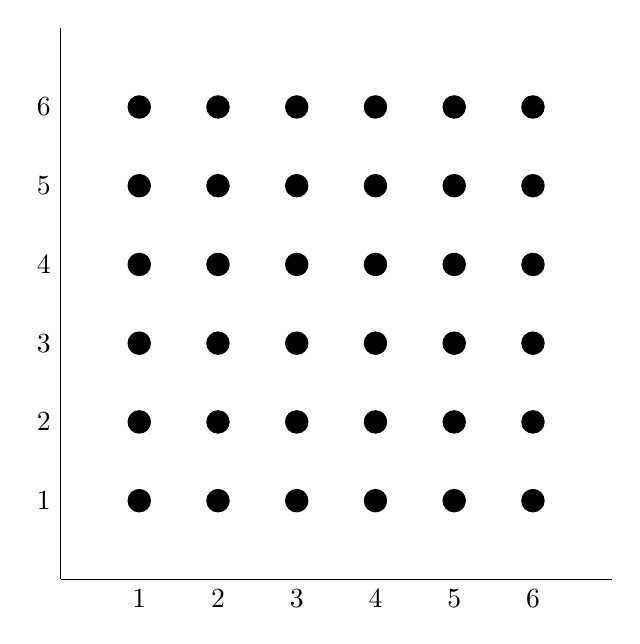
\begin{tikzpicture}[scale=1]
            \foreach \x in {1,...,6}
                {
                    \foreach \y in {1,...,6}
                        {
                            \node at (\x, \y)[circle,fill,inner sep=3pt]{};
                        }
                    \node[left] at (0, \x){$\x$};
                    \node[below] at (\x, 0){$\x$};
                }

            \draw (0.0, 0.0) -- (7.0, 0.0);
            \draw (0.0, 0.0) -- (0.0, 7.0);
        \end{tikzpicture}
    \end{center}

    为了证明这个格上无限多顶点是\textbf{可数}无限的,我们可以描述一条路径,该路径遍历所有的点(满射!)且每个点只遍历一次(单射!),并用自然数进行索引(可数无限!)。也就是说,我们可以描述一种通过一系列步骤遍历整个格上顶点的方式;会有一个``第一个点''和一个``第二个点''等等。

    关键的洞察是,这个格的左上对角线都是\textbf{有限的}。例如,从点 $(5, 1)$ 开始,向左上对角移动。你将经过 $(4, 2), (3, 3), (2, 4), (1, 5)$,然后到达格的边界。不论你从底部的哪一行开始,这都是正确的。

    让我们利用这一事实,根据 (a) 它所在的对角线,以及 (b) 它在该对角线上的位置,用自然数标记每个点。我们将从 $(1, 1)$ 开始的对角线视为第一条对角线,将从 $(2, 1)$ 开始的对角线视为第二条对角线,依此类推。这给了我们以下标注:

    \begin{center}
        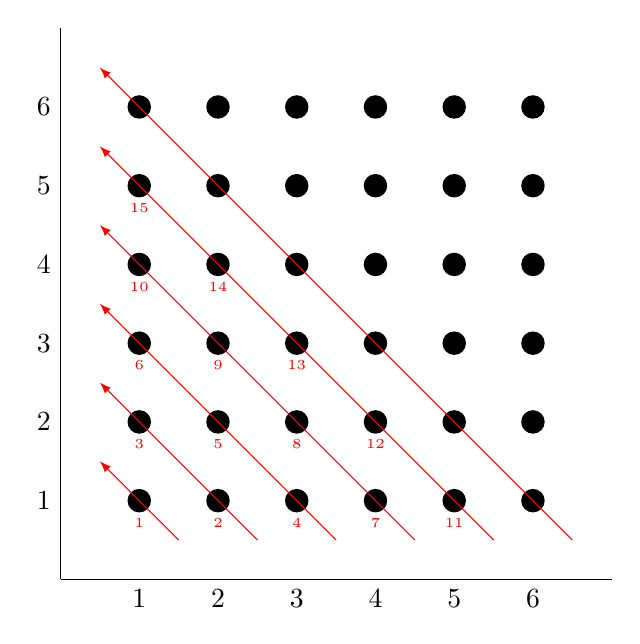
\begin{tikzpicture}[scale=1]
            \foreach \x in {1,...,6}
                {
                    \foreach \y in {1,...,6}
                        {
                            \node at (\x, \y)[circle,fill,inner sep=3pt]{};
                        }
                    \node[left] at (0, \x){$\x$};
                    \node[below] at (\x, 0){$\x$};
                    \draw[-latex, red] (\x+0.5, 0.5) -- (0.5, \x+0.5);
                }

            \draw (0.0, 0.0) -- (7.0, 0.0);
            \draw (0.0, 0.0) -- (0.0, 7.0);

            \foreach \y / \t in {1/1, 2/3, 3/6, 4/10, 5/15}
                {
                    \node[below,red] at (1, \y-0.1){\tiny$\t$};
                }
            \foreach \y / \t in {1/2, 2/5, 3/9, 4/14}
                {
                    \node[below,red] at (2, \y-0.1){\tiny$\t$};
                }
            \foreach \y / \t in {1/4, 2/8, 3/13}
                {
                    \node[below,red] at (3, \y-0.1){\tiny$\t$};
                }
            \foreach \y / \t in {1/7, 2/12}
                {
                    \node[below,red] at (4, \y-0.1){\tiny$\t$};
                }
            \node[below,red] at (5, 0.9){\tiny$11$};

        \end{tikzpicture}
    \end{center}

    我们可以看到,格中的每个顶点都会恰好落在某条对角线上。此外,这些对角线的数量是可数无限的(由 $\mathbb{N}$ 索引),而每条对角线上只有\emph{有限}多个点。这意味着(我们将在下面证明)所有对角线上的点的集合是可数无限集。

    你可以尝试通过定义一个函数来实现我们展示的标记方法,从而\emph{形式化}这个论点。或者,你也可以使用类似的方法,比如向右下方向移动,或者交替反转对角线的方向……
\end{example}

\begin{example}[$\mathbb{Q}$ 是可数无限集]

    这个结果是我们在处理无限集及其基数时,直觉失灵的一个显著例子。想象一下,把 $\mathbb{Q}$ 的元素分布在数轴上。它们似乎无处不在!事实上,回看练习 \ref{exc:exercises4.11.26},在那道练习中,你证明了有理数是\textbf{稠密的},这意味着在 $\mathbb{R}$ 中也是如此(即任意两个不同实数之间都存在一个有理数)。此外,有理数集\emph{看起来}比整数集 $\mathbb{Z}$ 大得多:仅在 $0$ 和 $1$ 之间,就有无穷多个有理数!出于这些原因,你可能会认为 $\mathbb{Q}$ 是不可数无限集,但这是错误的。

    在这个例子中,我们将提供几个论证来证明这一点,因为我们意识到这个结论确实非常奇特和炸裂。

    \begin{enumerate}[label=(\arabic*)]
        \item \textbf{直观解释:}\\
              考虑以下将 $\mathbb{Q}$ 表示为集合并集的形式:
              \[\mathbb{Q} \;\text{``}=\text{''}\; \big(\text{``}\mathbb{N} \times \mathbb{N}\text{''}\big) \cup \big(\text{``}-(\mathbb{N} \times \mathbb{N})\text{''}\big) \cup \{0\}\]
              某种意义上,$\mathbb{N} \times \mathbb{N}$ 可以对应所有正有理数。要理解这一点,只需考虑函数 $f : \mathbb{N} \times \mathbb{N} \to \mathbb{Q}_+$,定义为 $f(x, y) = \frac{x}{y}$。这个函数确实能够生成所有正有理数(因此 $f$ 是一个满射),但由于 $\frac{4}{2}=\frac{2}{1}$,所以它不是一个单射。因为 $f$ 是满射,这至少表明 $|\mathbb{N} \times \mathbb{N}| \ge |\mathbb{Q}|$。由于 $\mathbb{N} \times \mathbb{N}$ 是可数无限集,而 $\mathbb{Q}$ 显然也是无限集,这表明正有理数是可数无限集。\\

              负有理数集 $\mathbb{Q}_-$ 也具有与正有理数集 $\mathbb{Q}_+$ 相同的基数。它们之间存在明确的双射关系:定义函数 $g : \mathbb{Q}_+ \to \mathbb{Q}_-$ 为 $\forall q \in \mathbb{Q}_+ \centerdot g(q) = -q$。\\

              这里唯一遗漏的是 $0 \in \mathbb{Q}$。两个可数无穷集的并集仍然是可数无穷集(我们将在下面证明),再加上一个元素也不会改变这一点。因此,$\mathbb{Q}$ 是可数无限集。\\

              需要注意的是,这里有点``随意''。上面``等式''中的所有``引号''表示你应该仅将其作为启发性论证,而不是严格证明。然而,确实有方法可以使这些论证形式化。试着自己动手做做看吧!\\
        \item \textbf{列出 $\mathbb{Q}$ 中元素:}\\
              考虑编写一个计算机程序,列出所有正有理数。你会使用什么算法?只要你能保证你的程序``最终''会成功列出所有这些数,那么你就已经证明了 $\mathbb{Q}$ 可以一个一个地枚举出来,因此它必然是可数无限集。(这也是为什么我们使用 $\mathbb{N}$ 作为典型的可数无限集:我们可以一个一个地枚举它的元素,我们可以数它们。)\\

              这里有一种方法可以编写该程序:按照我们在前一个例子中使用 $\mathbb{N} \times \mathbb{N}$ ``格点路径''论证。这次,只需``跳过''已经打印过的有理数。\\

              也就是说,我们会先打印 $(1, 1) \leftrightarrow 1$,然后是 $(2, 1) \leftrightarrow 2$,再然后是 $(1, 2) \leftrightarrow \frac{1}{2}$,接着是 $(3, 1) \leftrightarrow 3$,依此类推……\\

              哦!我们需要跳过 $(2, 2) \leftrightarrow 1$。我们怎么知道的?因为我们已经打印过 $1$。我们怎么知道某个数已经打印过了?我们只需查看已经打印过的有理数列表,检查即将打印的数是否已经出现过。如果已经出现过,就跳过;如果没有,就打印它然后继续。\\

              在枚举过程中,这意味着对于我们经过的每个格点,我们只需检查\emph{有限的}项;也就是说,我们需要查看已经打印过的\emph{有限大的}有理数集合。这意味着在每一步打印过程中会花费``稍长一点的时间'',但不会\emph{无限长}。因此,我们的程序最终会列出每一个有理数;无论你想到的是哪个,我们都会在有限的时间内到达它。\\
        \item \textbf{$\mathbb{Q}$ 至多是可数无限集:}\\
              这是 $\mathbb{Q}$ 是可数集的另一个论证。(如果你觉得有点多余,那也没关系,可以跳过。我们只是觉得这个结果很有趣,从多个角度思考问题可能会有所帮助!)\\

              请思考一下:我们可以先验地认为 $|\mathbb{Q}| \ge |\mathbb{N}|$。这是因为 $\mathbb{Q} \supseteq \mathbb{N}$。现在,唯一的问题是这些基数是否相等。为了得出这个结论,我们需要找到
              \begin{enumerate}[label=(\alph*)]
                  \item 从 $\mathbb{Q}$ 到某个可数集的单射;
                  \item 从某个可数集到 $\mathbb{Q}$ 的满射。\\
              \end{enumerate}

              我们将在下面证明 $\mathbb{Z} \times \mathbb{N}$ 是可数的。(也就是说,我们将证明任意两个可数无限集的笛卡尔积也是可数无限集。)然后我们可以定义函数 $f : \mathbb{Z} \times \mathbb{N} \to \mathbb{Q}$ 为
              \[\forall (z, n) \in \mathbb{Z} \times \mathbb{N} \centerdot f(z, n) = \frac{z}{n}\]
              该函数是 $\mathbb{Q}$ 上的满射。虽然它肯定不是单射(为什么不是?)但这并不影响我们的结论。它表明 $|\mathbb{Z} \times \mathbb{N}| = |\mathbb{Q}|$。一旦我们证明了 $|\mathbb{Z} \times \mathbb{N}| = |\mathbb{N}|$,就可以得出 $|\mathbb{N}| = |\mathbb{Q}|$。\\
        \item \textbf{Stern-Brocot 树:}\\
              $\mathbb{Q}$ 还有其他视觉表示方法,其中 \textbf{Stern-Brocot 树}尤其具有启发性。这个概念最早由法国钟表匠 Achille Brocot 提出并发展,他在制作钟表时需要找到齿轮齿数的近似值。大约在同一时期($19$ 世纪 $50$ 年代和 $60$ 年代),德国数学家 Moritz Stern 也发展了这一想法。令人惊讶的是,一位非数学家竟然能\emph{独立地}发展出这样一个迷人的概念来解决实际问题!\\

              (不必过于担心\emph{图}和\emph{树}等术语。我们不会深入讨论它们,只是简单介绍一下,帮助理解 $\mathbb{Q}$ 的表示方法,并展示它是可数无穷集。)\\

              这棵树的\textbf{根节点}为 $1$。(即图中最顶端的数字。)\textbf{父节点和子节点的关系}(即如何生成树的下一层节点)是通过连分数定义的。(我们在这里不详细解释其含义,而是描述如何构建这棵树。)\\

              通过这种构造方法,从根节点到任一节点的路径会产生一系列有理数,这些有理数逐渐逼近最终的节点。此外,序列中的每个后续有理数的分母都比前一个大。这正是 Brocot 先生的动机所在。他需要确定手表内部两个齿轮的齿数,使它们的大小比率非常接近某个特定数值。通过沿着这棵树向下寻找,他可以找到更接近所需数值的近似比率!是不是很酷?

              \begin{center}
                  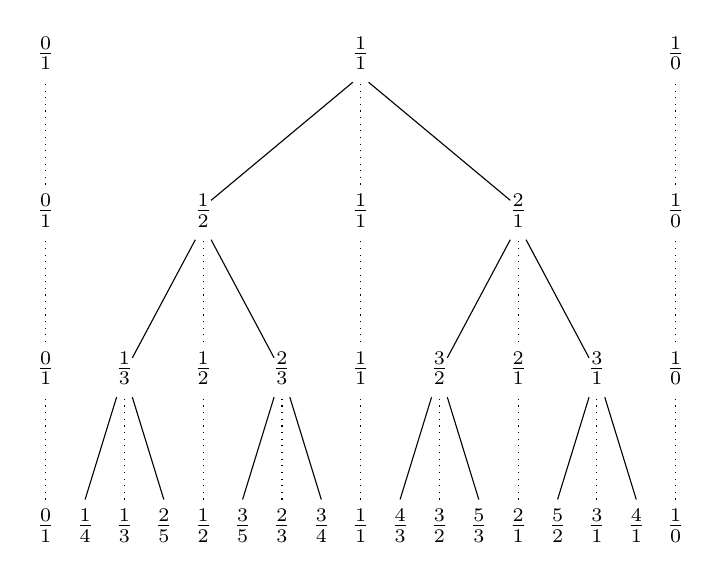
\begin{tikzpicture}[scale=1]
                      \edef \step {0.5};
                      \foreach \a / \b in {1/4, 1/3, 2/5, 1/2, 3/5, 2/3, 3/4}
                          {
                              \node[below] at (\step, 0){$\frac{\a}{\b}$};
                              \node[below] at (8-\step, 0){$\frac{\b}{\a}$};
                              \pgfmathparse{\step + 0.5};
                              \xdef \step{\pgfmathresult};
                          }

                      \edef \step {1.0};
                      \foreach \a / \b in {1/3, 1/2, 2/3}
                          {
                              \node[below] at (\step, 2){$\frac{\a}{\b}$};
                              \node[below] at (8-\step, 2){$\frac{\b}{\a}$};
                              \pgfmathparse{\step + 1.0};
                              \xdef \step{\pgfmathresult};
                          }

                      \node[below] at (2, 4){$\frac{1}{2}$};
                      \node[below] at (6, 4){$\frac{2}{1}$};

                      \foreach \y in {0,...,3}
                          {
                              \node[below] at (0, \y*2){$\frac{0}{1}$};
                              \node[below] at (4, \y*2){$\frac{1}{1}$};
                              \node[below] at (8, \y*2){$\frac{1}{0}$};
                          }

                      \edef \mx {0.1};
                      \edef \mya {0.2};
                      \edef \myb {0.7};
                      \foreach \y in {0,...,2}
                          {
                              \draw[dotted] (4, \y*2) -- (4, \y*2 + 2-\myb);
                          }

                      \foreach \x in {0,...,3}
                          {
                              \draw[dotted] (\x, 0.0) -- (\x, 2-\myb);
                              \draw[dotted] (8-\x, 0.0) -- (8-\x, 2-\myb);
                              \draw (\x*2+0.5, 0.0) -- (\x*2+1-\mx, 2-\myb);
                              \draw (\x*2+1.5, 0.0) -- (\x*2+1+\mx, 2-\myb);
                          }
                      \foreach \x in {0,...,1}
                          {
                              \draw[dotted] (\x*2, 2.0) -- (\x*2, 4-\myb);
                              \draw[dotted] (8-\x*2, 2.0) -- (8-\x*2, 4-\myb);
                              \draw (\x*4+1+\mx, 2.0-\mya) -- (\x*4+2-\mx, 4-\myb);
                              \draw (\x*4+3-\mx, 2.0-\mya) -- (\x*4+2+\mx, 4-\myb);
                          }
                      \foreach \x in {0}
                          {
                              \draw[dotted] (\x*8, 4.0) -- (\x*8, 6-\myb);
                              \draw[dotted] (8-\x*8, 4.0) -- (8-\x*8, 6-\myb);
                              \draw (\x*8+2+\mx, 4.0-\mya) -- (\x*8+4-\mx, 6-\myb);
                              \draw (\x*8+6-\mx, 4.0-\mya) -- (\x*8+4+\mx, 6-\myb);
                          }
                  \end{tikzpicture}
              \end{center}

              为了实际\emph{构建}这棵树,我们需要找到\emph{中位数}。给定两个有理数 $\frac{a}{b}$ 和 $\frac{c}{d}$,它们的中位数定义为 $\frac{a+b}{c+d}$。(注意,这里的中位数指的是一种特殊的对象;这\emph{不是}两个分数相加的正确方法!)\\

              树的每一层由上一层中相邻有理数对的所有中位数组成;我们不``计算''直接垂直的元素,它们只是为了便于阅读和构建而保留的。此外,注意分数 $\frac{0}{1}$ 和 $\frac{1}{0}$(尽管 $\frac{1}{0}$ 是未定义的!)包含在外侧列中,用于辅助生成每层最外侧的元素。\\

              (可以尝试探索这棵树的性质,并阅读更多\href{https://en.wikipedia.org/wiki/Stern%E2%80%93Brocot_tree}{相关内容}。这是一个非常有趣的数学对象!)\\

              我们在这里不会证明这棵树包含\emph{所有}有理数,但我们相信你可以理解为什么这是可信的。此外,我们也相信你可以理解为什么这棵树中的所有节点集合是\textbf{可数}无限集。每一层只有有限多个节点,而层数是可数无穷多层。
    \end{enumerate}

\end{example}

\subsubsection*{定理}

现在我们知道,$\mathbb{N}, \mathbb{Z}, \mathbb{Q}$ 这三个标准数集,以及 $\mathbb{N} \times \mathbb{N}$,都是可数无限集。接下来,通过一些定理,我们将展示如何从这些已有集合中生成更多的可数无限集。

我们先来看一个有用的结论。这个结论表明,如果我们在一个可数无限集上``添加''有限多个元素,结果仍然是可数无限集。

\begin{lemma}\label{lemma7.6.16}
    如果 $A$ 是可数无限集,$B$ 是有限集且 $A \cap B = \varnothing$,则 $A \cup B$ 为可数无限集。
\end{lemma}

\begin{proof}
    留作练习 \ref{exc:exercises7.8.19}

    (\textbf{提示}:采用与证明定理 \ref{theorem7.6.7} 类似的思路。)
\end{proof}

\begin{remark}
    注意:在这个引理中,假设 $A \cap B = \varnothing$ 并非\emph{必要},但它可以简化证明过程。

    当 $A \cap B \ne \varnothing$ 时,我们可以将刚刚证明的结果应用到集合 $A - B$(它是可数无限集)和 $B - A$(它是有限集)上,从而得到可数无限的集 $(A - B) \cup (B - A)$(因为它们是互斥的)。然后,我们可以再次将上述结论应用于该集合 --- $(A - B) \cup (B - A)$ --- 和 $A \cap B$,从而得到可数无限集:
    \[A \cup B = (A - B) \cup (B - A) \cup (A \cap B)\]
\end{remark}

下一个结论表明,该方法同样适用于 $A$ 和 $B$ 都是可数无限集的情况。

\begin{lemma}\label{lemma7.6.18}
    如果 $A$ 和 $B$ 都是可数无限集,且 $A \cap B = \varnothing$,则 $A \cup B$ 为可数无限集。
\end{lemma}

\begin{proof}
    因为 $A$ 和 $B$ 为可数无限集,则存在双射 $ f : A \to \mathbb{N}$ 和 $g : B \to \mathbb{N}$。给定这样的函数,我们要找到 $h : A \cup B \to \mathbb{N}$。

    首先定义函数 $p : \mathbb{N} \to \mathbb{Z} - \mathbb{N}$ 为 $\forall n \in \mathbb{N} \centerdot p(n) = -n + 1$。

    这是一个双射,因为 $p^{-1} : \mathbb{Z} - \mathbb{N} \to \mathbb{N}$ 为 $p^{-1}(z) = -z + 1$。(请你自行验证!)

    由于 $p$ 和 $g$ 都是双射,所以 $p \circ g : \mathbb{Z} - \mathbb{N}$ 也为双射。

    接着我们定义分段函数 $q : A \cup B \to \mathbb{Z}$ 为
    \[\forall x \in A \cup B \centerdot q(x) = \begin{cases}
            f(x)    & \text{如果}\; x \in A \\
            p(g(x)) & \text{如果}\; x \in B
        \end{cases}\]
    这是一个良好定义的函数,因为 $A \cap B = \varnothing$。此外,这也是一个双射函数,因为每一段函数都是双射。(请你自行检验以确保它是合理的。另外,请参见练习 \ref{exc:exercises7.8.31},那里给出了一般情况下的证明。)

    综上,我们知道如何构建双射 $r : \mathbb{Z} \to \mathbb{N}$。(还记得我们是怎么做的吗?请参考示例 \ref{ex:example7.6.12}。)

    最后,定义函数 $h : A \cup B \to \mathbb{N}$ 为 $h = r \circ q$。这个函数是双射的复合,因此也是双射。这证明了 $ |A \cup B| = |\mathbb{N}|$,即 $A \cup B$ 为可数无限集。
\end{proof}

接下来的推论表明,实际上我们不需要假设 $A \cap B = \varnothing$。这个假设只是为了让证明过程更简单。我们希望你能证明这个推论。

\begin{corollary}\label{corollary7.6.19}
    如果 $A$ 和 $B$ 都是可数无限集,则 $A \cup B$ 为可数无限集。
\end{corollary}

\begin{proof}
    留作练习 \ref{exc:exercises7.8.20}。

    (\textbf{提示}:将引理 \ref{lemma7.6.18} 应用于适当的集合上……)
\end{proof}

以上证明了几个关于集合\emph{并集}的情况。接下来我们来证明一个关于\emph{笛卡尔积}的结论。

\begin{theorem}
    如果 $A$ 和 $B$ 都是可数无限集,则 $A \times B$ 为可数无限集。
\end{theorem}

这个证明其实很简单,因为我们已经证明了关于 $\mathbb{N} \times \mathbb{N}$ 结论。这个集合是笛卡尔积,并且是可数无穷集。请看我们在证明中如何使用 $\mathbb{N} \times \mathbb{N}$:

\begin{proof}
    假设 $A$ 和 $B$ 为可数无限集,则存在双射 $ f : A \to \mathbb{N}$ 和 $g : B \to \mathbb{N}$。给定这样的函数。

    定义函数 $h : A \times B \to \mathbb{N} \times \mathbb{N}$ 为
    \[\forall (x, y) \in A \times B \centerdot h(x, y) = \big(f(x), g(y)\big)\]
    我们声称这是一个双射函数。因为 $f, g$ 都是可逆的,定义函数 $H : \mathbb{N} \times \mathbb{N} \to A \times B$ 为
    \[\forall (k, \ell) \in \mathbb{N} \times \mathbb{N} \centerdot H(k, \ell) = \big(f^{-1}(k), g^{-1}(\ell)\big)\]
    我们声称 $H = h^{-1}$。因为
    \begin{align*}
        \forall (x, y) \in A \times B \centerdot (H \circ h)(x, y) & = H(h(x, y)) = H \big(f(x), g(y)\big)           \\
                                                                   & = \big(f^{-1}(f(x)), g^{-1}g((y))\big) = (x, y)
    \end{align*}
    且
    \begin{align*}
        \forall (k, \ell) \in \mathbb{N} \times \mathbb{N} \centerdot (h \circ H)(k, \ell) & = h(H(k, \ell)) = h\big(f^{-1}(k), g^{-1}(\ell)\big)  \\
                                                                                           & = \big(f(f^{-1}(k)), g(g^{-1}(\ell))\big) = (k, \ell)
    \end{align*}
    所以 $H \circ h = \id_{A \times B}$ 且 $h \circ H = \id_{\mathbb{N} \times \mathbb{N}}$。这表明 $H = h^{-1}$。

    因此,$h$ 为双射。所以 $|A \times B| = |\mathbb{N} \times \mathbb{N}| = |\mathbb{N}|$。
\end{proof}

通过对前两个结论进行归纳,我们可以证明以下推论:

\begin{corollary}\label{corollary7.6.21}
    假设 $A_1, \dots , A_n$ 为可数集(其中 $n \in \mathbb{N}$,所以我们有可数无限个集合),则 $A_1 \cup \dots \cup A_n$ 和 $A_1 \times \dots \times A_n$ 为可数无限集
\end{corollary}

\begin{proof}
    留作练习 \ref{exc:exercises7.8.22}。
\end{proof}

\subsubsection*{可数个可数集的并集为可数集}

你可能会好奇,当我们对\emph{可数无穷多}个集合(每个集合都是可数无限集)进行并集或乘积运算时,会发生什么情况。让我们先来探讨并集的情况。这个结果非常基础且重要,我们甚至在章节标题中重复强调了它!

\begin{theorem}\label{theorem7.6.22}
    对于每个 $n \in \mathbb{N}$,假设我们有 $A_n$ 为可数无限集,则集合
    \[A = \bigcup_{n \in \mathbb{N}} A_n = A_1 \cup A_2 \cup A_3 \cup \dots\]
    为可数无限集。
\end{theorem}

我们将证明集合\textbf{互不相交}的情况,剩下的细节留给你来处理。

\begin{proof}
    对于每个 $n \in \mathbb{N}$,假设我们有 $A_n$ 为可数无限集,且 $\forall i, j \in \mathbb{N} \centerdot i \ne j \implies A_i \cap A_j = \varnothing$。定义
    \[A = \bigcup_{n \in \mathbb{N}} A_n\]
    我们声称 $A$ 为可数无限集。

    因为每一个 $A_n$ 都是有限可数集,我们知道对于每一个 $n \in \mathbb{N}$ 存在双射 $f_n : A_n \to \mathbb{N}$。这使得我们能够根据双射 $f_n$ 的定义对每一个集合 $A_n$ 的元素进行``编号''。此外,我们对 $A_n$ 集合进行编号,这些集合由 $\mathbb{N}$ 索引。本质上,我们对 $A$ 的元素进行了``编号'',这些编号对应于 $\mathbb{N} \times \mathbb{N}$。接下来我们将正式定义这种对应关系。

    我们定义函数 $F : A \to \mathbb{N} \times \mathbb{N}$。给定任意 $x \in A$,我们知道 $\exists n \in \mathbb{N} \centerdot x \in A_n$ 且 $n$ 是\emph{唯一的}。(这是因为给定的集合是互不相交的)。设 $F(x) = \big(n, fn(x)\big)$。

    我们声称 $F$ 为双射。考虑函数 $G : \mathbb{N} \times \mathbb{N} \to A$ 定义为
    \[\forall (a, b) \in \mathbb{N} \times \mathbb{N} \centerdot G(a, b) = f_a^{-1}(b)\]
    也就是说,$G$ 使用第一个坐标 $a$ 来确定集合 $A_a$,然后使用函数 $f_a$ 来确定 $A_a$ 中输出 $b \in \mathbb{N}$ 的元素。

    (留给读者验证 $G = F^{-1}$。)

    这表明 $|A| = |\mathbb{N} \times \mathbb{N}| = |\mathbb{N}|$,所以 $A$ 是可数无限集。

    $A_n$ 可能相交的情况,留作练习 \ref{exc:exercises7.8.37}。
\end{proof}

\begin{corollary}\label{corollary7.6.23}
    对于每个 $n \in \mathbb{N}$,假设我们有 $A_n$ 为有限集,且这些集合互不相交。定义集合
    \[A = \bigcup_{n \in \mathbb{N}} A_n\]
    则 $A$ 为可数有限集。
\end{corollary}

\begin{proof}
    留作练习 \ref{exc:exercises7.8.36}。
\end{proof}

这个结论非常强大。让我们两个应用示例。\\

\begin{example}[所有质数幂次的集合]
    还记得希尔伯特旅馆的讨论吗?在那个例子中,我们容纳了无穷多个会议,每个会议的人数也是无穷的。我们将客人们安排到对应质数幂次的房间。对于每一个 $n \in \mathbb{N}$,定义 $p_n$ 为第 $n$ 个质数。则
    \[A_n = \{p_n^k \mid k \in \mathbb{N}\}\]
    为第 $n$ 个质数所有幂次的集合。上面的定理告诉我们
    \[\bigcup_{n \in \mathbb{N}} A_n = \{\text{质数的所有幂次}\}\]
    也是可数无限集。确实,这并不意外,因为上面的并集只是自然数的一个子集,而自然数本身是可数无限集!
\end{example}

\begin{example}[所有有限长二进制字符串的集合]\label{ex:example7.6.25}
    二进制字符串被定义为由 \verb|0| 和 \verb|1| 组成的有序序列。\textbf{有限长二进制字符串}是指长度有限的二进制字符串。

    例如,下面这些都是有限长二进制字符串:
    \[0, \quad 1, \quad 101010, \quad 10000000000000000001 \]

    对于每个 $n \in \mathbb{N}$,定义 $F_n$ 为所有长度为 $n$ 的二进制字符串的集合。例如
    \begin{align*}
        F_1 & = \{ 0 , 1 \}                                         \\
        F_2 & = \{ 00 , 01 , 10 , 11 \}                             \\
        F_3 & = \{ 000 , 001 , 010 , 100 , 011 , 101 , 110 , 111 \}
    \end{align*}
    依此类推。(注意 $|F_n| = 2^n$。试着证明一下。)则定义所有有限长二进制字符串的集合为
    \[F = \bigcup_{n \in \mathbb{N}} F_n\]

    $F$ 的每个元素必须来自大并集中的某个集合;这意味着任意元素 $x \in F_n$ 都是某个具有有限长度的二进制字符串。这个长度可能非常大,但它是有限的。(这说明了``任意大(但有限)''和``无限''之间的区别。)

    这个例子的重点是,根据上面的定理,$F$ 是可数的!(实际上,这是从紧随其后的推论得出的。)相比之下,所有\emph{无限长}二进制字符串的集合 $S$ 是不可数的 --- 我们很快会证明这一点。我们将经常使用这些二进制字符串集合作为例子!
\end{example}

\subsubsection*{取``极限''}

我们已经证明,如果 $A$ 和 $B$ 是可数无限集,那么 $A \cup B$ 和 $A \times B$ 也是可数无限集。我们还建议你使用归纳法(对并集或乘积中的集合数量进行归纳)来证明,对于任意 $n \in \mathbb{N}$,
\[A_1 \cup A_2 \cup \dots \cup A_n = \bigcup_{i \in [n]} A_i \quad \text{和} \quad \prod_{i \in [n]} A_i = A_1 \times A_2 \times \dots \times A_n\] 
也是可数无限集。

这些结论是否为我们提供了某些关于
\[A_1 \cup A_2 \cup A_3 \cup \dots = \bigcup_{k \in \mathbb{N}} A_k\]
和
\[A_1 \times A_2 \times A_3 \times \dots = \prod_{k \in \mathbb{N}} A_k\]
的信息?也就是说,当我们尝试从\emph{有限}数量的并集/乘积(任意大但仍然有限)过渡到\emph{无限}数量的并集/乘积时,会发生什么?我们能得出必要的结论吗?我们能找到反例吗?

主要思想是,``取极限''确实会创建某些数学对象,但我们不能预先假设这个对象具有与定义它的序列中所有对象\emph{完全相同的属性}。

考虑有限集 $[n]$,对于每个 $n$,它们都是有限的,但``取极限''后我们得到的 $\mathbb{N}$ 是无限的。所以我们确实得到了一个对象(另一个集合),但它不一定具有相同的属性。

上述重要定理表明,在\emph{并集}中取极限肯定会保留可数性。正如我们将在下一节中看到的那样,\emph{乘积}肯定\textbf{不会}保留可数性。(实际上,即使是无限个有限集的乘积也是不可数的。真是令人惊讶!)

在微积分中也有类似的概念。我们本来承诺不使用微积分,但这些思想之间有如此自然的关系,所以我们不得不提及一个简单的例子。如果你不理解也没关系;如果你理解了,试着记住这个联系,并思考它如何从根本上改变了你在微积分中学到的一切。)

考虑如下\emph{极限}:
\[\lim_{x \to \infty} \frac{1}{x} = 0\]
这个极限在什么意义上\textbf{等于} $0$?为什么身为资深数学家的我们会选择用这种方式\emph{定义}极限?形式上,这个极限是有意义的,因为它符合极限的量化定义。设 $P$ 为正实数集,极限的定义(应用于这个例子)为
\[\forall \varepsilon \in P \centerdot \exists M \in \mathbb{N} \centerdot \forall n \in \mathbb{N} \centerdot \big(n > M \implies \big|\frac{1}{x}\big| < \varepsilon \big)\]
也就是说,对于任何小的正阈值($\varepsilon > 0$),我们都可以找到一个特定的截止点(一个依赖于 $\varepsilon$ 的大自然数 $M$),使得 $M$ \emph{之后}的每一点,函数 $\frac{1}{x}$ 都在极限点 $0$ 的 $\varepsilon$ 阈值内。

请注意,这与 ``$\frac{1}{\infty} = 0$'' 这样的说法\emph{完全不同}。事实并非如此。实际上,我们从未真正``代入''极限的终点来进行计算。极限是通过量化定义的,也就是说,我们讨论的是在\emph{任意大}值下发生的情况,而不是在\emph{无限大}值下发生的情况。

% !TeX root = ../../../book.tex

\subsection{不可数集}

为了开始讨论不可数集,让我们证明一个之前提到过的结果。具体来说,我们将证明集合的可数无限次\emph{笛卡尔积}是不可数无限的。注意,我们甚至不需要这些集合是无限集:我们可以让它们都是大小为 $2$ 的有限集!在下一部分,我们将用这个结果展示一些不可数集的例子,包括一个我们已经熟悉的集合……

\subsubsection*{不可数笛卡尔积}

\begin{theorem}
    双元素集合的可数无限次笛卡尔积是不可数无限的。也就是说
    \[\{0, 1\}^{\mathbb{N}} = \{0, 1\} \times \{0, 1\} \times \{0, 1\} \times \dots\]
    是不可数无限集。
\end{theorem}

\begin{proof}
    为了得到矛盾而假设 $\{0, 1\}^{\mathbb{N}}$ 是可数无限集。这意味着我们可以找到该集合和 $\mathbb{N}$ 之间的双射。也就是说,我们可以将该集合中的所有元素与自然数一一对应起来。因此,这个集合有第一个元素,对应于自然数 $1$;有第二个元素,对应于自然数 $2$;依此类推。

    虽然我们并不确切知道这些元素具体是什么,但可以确定这种对应关系确实存在。我们可以将 $\{0, 1\}^{\mathbb{N}}$ 的所有元素 $y_i$ 列出来。每个 $y_i$ 是一个由 $0$ 和 $1$ 组成的有序无限列表,因此可以这样表示:
    \begin{align*}
        1 & \leftrightarrow (a_{1,1} , a_{1,2} , a_{1,3} , a_{1,4} , a_{1,5} , \dots) = y_1 \\
        2 & \leftrightarrow (a_{2,1} , a_{2,2} , a_{2,3} , a_{2,4} , a_{2,5} , \dots) = y_2 \\
        3 & \leftrightarrow (a_{3,1} , a_{3,2} , a_{3,3} , a_{3,4} , a_{3,5} , \dots) = y_3 \\
        4 & \leftrightarrow (a_{4,1} , a_{4,2} , a_{4,3} , a_{4,4} , a_{4,5} , \dots) = y_4 \\
        5 & \leftrightarrow (a_{5,1} , a_{5,2} , a_{5,3} , a_{5,4} , a_{5,5} , \dots) = y_5 \\
          & \vdots
    \end{align*}
    每个值 $a_{i,j}$ 要么是 $0$,要么是 $1$。$i$ 表示我们对应的是哪个自然数(也就是列表中的\emph{垂直}位置),而 $j$ 则表示我们在哪个坐标(也就是列表中的\emph{水平}位置)。

    因为我们假设这个对应关系是双射,所以这个列表包含了 $\{0, 1\}^{\mathbb{N}}$ 的所有元素。为了完成反证法,我们将构造一个 $\{0, 1\}^{\mathbb{N}}$ 的元素,并确保它\textbf{不会}出现在这个列表中!(这就是康托对角线论证的一种形式。)

    我们定义对象 $x = (x_1, x_2, x_3, \dots)$ 为
    \[x_i = \begin{cases}
            0 & \text{如果}\; a_{i,i} = 1 \\
            1 & \text{如果}\; a_{i,i} = 0
        \end{cases}\]
    也就是说,我们通过沿着元素矩阵的\emph{主对角线}向下构建 $x$(这样我们可以看到所有的元素 $a_{i,i}$),并将值从 $1$ \emph{切换为} $0$,或从 $0$ 切换为 $1$。

    下图是一个\emph{具体示例},展示了如何执行这个操作,虽然它不是一般性证明的一部分,但为了更好地说明,我们将其包含在内:
    \begin{align*}
        1 & \leftrightarrow (\circled{1} , 1 , 0 , 0 , 1 , \dots) = y_1                        \\
        2 & \leftrightarrow (1 , \circled{0} , 0 , 0 , 1 , \dots) = y_2                        \\
        3 & \leftrightarrow (0 , 0 , \circled{1} , 1 , 0 , \dots) = y_3                        \\
        4 & \leftrightarrow (1 , 1 , 0 , \circled{1} , 1 , \dots) = y_4                        \\
        5 & \leftrightarrow (0 , 1 , 1 , 1 , \circled{0} , \dots) = y_5                        \\
          & \vdots                                                                             \\
        x & =\big(\circled{0}, \circled{1}, \circled{0}, \circled{0}, \circled{1}, \dots \big)
    \end{align*}
    我们为什么要这样做?思考一下,对象 $x$ 是否可能属于上面提到的元素列表。
    \begin{itemize}
        \item $x = y_1$ 吗?不相等!因为 $x$ 与 $y_1$ 的第一个坐标不同。(在本例中,$x_1=0$ 而 $y_{1,1} = 1$。)
        \item $x = y_2$ 吗?不相等!因为 $x$ 与 $y_2$ 的第二个坐标不同。(在本例中,$x_2=1$ 而 $y_{2,2} = 0$。)
        \item $x = y_3$ 吗?不相等!因为 $x$ 与 $y_3$ 的第三个坐标不同。(在本例中,$x_3=0$ 而 $y_{3,3} = 1$。)
    \end{itemize}
    一般来讲,对于任意 $i \in \mathbb{N}$,我们可以保证 $x$ 和 $y_i$ 在第 $i$ 个坐标上是不同的。因此,\textbf{没有}一个 $y_i$ 对象等于这个新对象 $x$。也就是说
    \[\big(\forall i \in \mathbb{N} \centerdot x_i \ne y_{i,i}\big) \implies \big(\forall i \in \mathbb{N} \centerdot x \ne yi\big)\]
    但是根据我们对 $x$ 的定义,它确实是一个有序无限的 $0, 1$ 列表,所以它必然是 $\{0, 1\}^{\mathbb{N}}$ 的一个元素。

    这就产生了一个矛盾。我们假设可以列出集合中的所有元素,但随后我们用这种顺序构造了一个集合中的元素,而这个元素显然不在列表中。$\hashx$

    因此 $\{0, 1\}^{\mathbb{N}}$ 为不可数无限集。
\end{proof}

请注意:这是一个非常巧妙的论证。这是我最喜欢的数学证明之一。康托尔真是个天才,他想出了这个证明,更有趣的是,这个证明实际上相当简单且令人难忘。我们相信你不会忘记这个``沿主对角线切换值''的论证。我们甚至可以用八个字总结整个证明,这进一步彰显了它的精彩。

\begin{corollary}
    任意至少两个元素的集合的可数无限次笛卡尔积是不可数无限的。
\end{corollary}
(注意:我们实际上只需要说明乘积中的集合都不为空,且其中只有有限多个集合可以只有一个元素。)

\subsubsection*{示例}

你可能会好奇:什么样的集合是不可数无限的呢?我们知道这样的集合吗?当然知道!下面是一些例子。\\

\begin{example}[所有无限长二进制字符串的集合]

    你可能已经注意到,我们在上面证明中使用的集合 --- 即 $\{0, 1\}^\mathbb{N}$ --- 实际上就是无限长二进制字符串集合 $S$!$\{0, 1\}^\mathbb{N}$ 中的元素是无限长的有序序列,每个位置上的值都是 \verb|0| 或 \verb|1|。$S$ 中的元素也是无限长的 \verb|0| 和 \verb|1| 的有序序列,只是不包含括号和逗号。因此,这两者之间存在一个非常自然的双射关系(只需去掉括号和逗号,或者再加上它们),所以我们将这两个集合视为相同集合。

    我们在上面的示例 \ref{ex:example7.6.25} 中看到,所有有限长二进制字符串的集合是可数无限集。最新的结果表明,所有无限长二进制字符串的集合是不可数无限集。另一种证明这一事实的方法是找到 $S$ 和 $\mathcal{P}(\mathbb{N})$ 之间的双射关系,然后应用康托尔定理,该定理表明 $|\mathbb{N}| < |\mathcal{P}(\mathbb{N})|$。(详见练习 \ref{exc:exercises7.8.33}。)
\end{example}

\begin{example}[$\mathbb{R}$ 是不可数无限集]

    这是我们第一次接触到一个不可数无限的标准数集。我们可以用上面的结论来证明这一点。

    这个说法在直觉上是合理的,因为实数轴看起来比自然数集 $\mathbb{N}$ 或整数集 $\mathbb{Z}$ 大得多。但我们也知道,有理数集 $\mathbb{Q}$ 是可数无限集,并且在实数轴上有无数个有理数存在。实际上,\emph{在任意两个实数}之间都有无限多个有理数。

    我们将看到,实数集 $\mathbb{R}$ 确实是不可数无限集。此外,我们还会证明 $\mathbb{R}$ 和幂集 $\mathcal{P}(\mathbb{N})$ 具有相同的``无限大小'';也就是说,我们将证明 $|\mathbb{R}| = |\mathcal{P}(\mathbb{N})|$。 (请记住,这比仅仅说两个集合都是不可数集具有更多信息量;不可数无限集有很多级别,我们暂时不深入讨论这些,以免让我们头脑爆炸。)

    直观上,要理解 $\mathbb{R}$ 是不可数无限集,首先可以将 $\mathbb{R}$ 与集合 $\{0, 1, 2, 3, 4, 5, 6, 7, 8, 9\}^\mathbb{N}$ 联系起来。每个实数都可以用十进制表示,这实际上就是一个有序的、可数无限的数字列表。虽然在十进制表示中会出现像 $0.999999 \dots = 1$ 这样的问题,但这些问题并不重要。既然我们已经知道,即便像 $\{0, 1\}$ 这样的小集合,当我们无限次地取其乘积时,也会生成一个不可数集合,那么一个更大的集合,比如 $\{0, 1, \dots , 9\}$,也必定会生成一个不可数集合。这个直观的论证可以帮助你理解并向朋友解释这个结论。(事实上,大多数教科书中也是这样解释的。)

    更正式地,我们可以证明 $|\mathbb{R}| = |\mathcal{P}(\mathbb{N})|$。这个更强的结论意味着 $\mathbb{R}$ 是不可数无限集(因为康托尔定理告诉我们 $|\mathbb{N}| < |\mathcal{P}(\mathbb{N})|$)。为此,我们考虑集合
    \[I = \{y \in \mathbb{R} \mid 0 \le y \le 1\}\]
    即区间 $[0, 1] \subseteq \mathbb{R}$。我们将证明
    \[|{0, 1}^\mathbb{N}| = |\mathcal{P}(\mathbb{N})| = |I|\]
    然后再应用一些关于区间与 $\mathbb{R}$ 之间存在双射的结论。

    考虑函数 $f_1 : \{0, 1\}^{\mathbb{N}} \to I$,它输入一个无限长二进制字符串,在这个二进制字符串的前面加上一个小数点,并将其作为\textbf{十进制}表示进行评估。

    例如,考虑元素 $(1, 1, 0, 0, 1, 0, \dots)$,其余部分为 $0$。则
    \[f_1(1, 1, 0, 0, 1, 0, \dots) = 0.110010 \dots _\text{DEC} = \frac{1}{10^1}+\frac{1}{10^2}+\frac{1}{10^5} = \frac{11001}{100000}\]
    请注意,这确实是一个函数,因为它的任何输出都必然是一个实数(因为它有小数表示法;我们刚刚给出了它),并且它的值介于 $0$ 和 $1$ 之间,这是因为我们把小数点放在了最前面。此外,请注意函数 $f_1$ 是\textbf{单射};两个不同的无限长二进制字符串在某些位置上必定不同,因此它们表示的小数在某些地方也会不同,从而不可能是相同的实数。这表明 $|\{0,1\}^{\mathbb{N}}| \le |I|$。

    考虑函数 $f2 : \{0, 1\}^{\mathbb{N}} \to I$,它输入一个无限长二进制字符串,在这个二进制字符串的前面加上一个小数点,并将其作为\textbf{二进制}表示进行评估。

    例如,考虑上面提到的相同元素。则
    \[f_2(1, 1, 0, 0, 1, 0, \dots) = 0.110010 \dots _\text{BIN} = \frac{1}{2^1}+\frac{1}{2^2}+\frac{1}{2^5} = \frac{25}{32}\]
    请注意,这确实是一个函数,因为它的任何输出都必然是一个实数;只需计算分数求和的结果,就会得到一个介于 $0$ 和 $1$ 之间的实数(即使序列是无限的,它也保证收敛)。例如,输入全是 $0$ 时,输出为 $0$;输入全是 $1$ 时,输出为 $1$,因为
    \[\frac{1}{2}+\frac{1}{4}+\frac{1}{8}+\dots = \sum_{k \in \mathbb{N}} \frac{1}{2^k} = 1\]
    此外,请注意,函数 $f_2$ 是\textbf{满射}。这一事实依赖于一些关于有理数和无理数的外部知识;具体来说,任何无理数都可以通过一系列二进制有理数(分母为 $2$ 的幂的有理数)来逼近。我们不会详细阐述或证明这些结论,但我们认为通过一些例子,你会逐渐理解其中的原理。事实上,搜索一下无理数的二进制展开形式,你会发现一些有趣的结果。

    因为 $f_2$ 是满射,这表明 $|\{0,1\}^{\mathbb{N}}| \ge |I|$。综上,我们得出结论 $|\{0,1\}^{\mathbb{N}}| = |I|$。我们还知道 $|\mathcal{P}(\mathbb{N})| = |\{0, 1\}^{\mathbb{N}}|$(见练习 \ref{exc:exercises7.8.33}),所以我们知道 $|I| = |\mathcal{P}(\mathbb{N})|$。

    最后一步是证明 $|I| = |\mathbb{R}|$。回看 \ref{sec:section7.5.4} 节中的练习 \ref{exc:exercises7.5.5}。在那里我们找到了集合 $J = \{y \in \mathbb{R} \mid -1 < y < 1\}$ 和 $\mathbb{R}$ 之间的双射。很容易找到集合 $J$ 和集合 $K = \{y \in \mathbb{R} \mid 0 < y < 1\}$ 之间的双射(不妨现在试一下!)。这表明 $|\mathbb{R}| = |J| = |K|$。此外,$K \subseteq I$,他们之间唯一的区别在于 $0$ 和 $1$ 这两个元素,因此 $K| = |I|$。最终,我们证明了 $|I| = |\mathbb{R}|$。因此,我们可以得出如下结论
    \[|\mathbb{R}| = |\mathcal{P}(\mathbb{N})|\]
    我们来看一下之前提到的两个论证:
    \begin{itemize}
        \item 考虑集合 $\{0, 1, 2, 3, 4, 5, 6, 7, 8, 9\}^\mathbb{N}$
        \item 考虑集合 $\{0, 1\}^\mathbb{N}$
    \end{itemize}
    这两个论证都涉及到一些关于十进制展开和二进制展开的知识。似乎没有简单的方法绕过这一点,所以我们希望上述结果仍然是令人信服的。特别是,你可以思考一下上面讨论中 $f_2$ 是\textbf{满射}但不是\textbf{单射}的结论。你能说服自己接受这个观点吗?你能说服别人吗?
\end{example}

\subsubsection*{定理}

让我们来看一个关于不可数集的结论。然后,在继续之前,我们会陈述一个关于无限集的最终定理。

\begin{lemma}\label{lemma7.6.29}
    假设 $A$ 为不可数无限集,$B$ 为可数无限集,且 $B \subseteq A$。则 $A-B$ 为不可数无限集。
\end{lemma}

(注意:我们\emph{不需要}假设 $B \subseteq A$。如果不是这种情况,可以将 $A$ 和 $B \cap A$ 作为集合来考虑。)

\begin{proof}
    留作 \ref{sec:section7.6.5} 节练习 \ref{exc:exercises7.6.5}。

    (\textbf{提示}:采用反证法……)
\end{proof}

\subsubsection*{识别无限集}

为了定义\textbf{无限集},我们首先定义了\textbf{有限集},然后称任何\emph{不是}有限集的集合都是无限集。下面的定理展示了另一种定义\textbf{无限集}的方法。具体来说,我们可以说一个集合是无限集,当且仅当我们能够找到一个双射,使其映射到自身的一个真子集。首先,让我们陈述并证明一个有用的引理;我们将在接下来的定理证明中用到它。

\begin{lemma}\label{lemma7.6.30}
    设 $A$ 为任意集合。则 $A$ 为无限集 $\iff$ 存在 $B \subset A$ 为可数无限集。
\end{lemma}

\begin{proof}
    $\impliedby$ 方向很明显。如果 $A$ 比某个无限集更大,它当然也是无限集。

    $\implies$ 方向则更有趣一些。假设 $A$ 为无限集。设 $\bigstar \in A$ 为某个特定元素。我们将其排除在外,并构造一个不包含 $\bigstar$ 且是可数无限的集合 $B$。这样就能保证 $B \subset A$,同时 $B \ne A$。

    考虑集合 $A_1 = A - \{\bigstar\}$。这个集合也是无限集,所以我们可以选择某个元素 $b_1 \in A_1$。

    考虑集合 $A_2 = A_1- \{b_1\} = A - \{\bigstar, b_1\}$。这个集合也是无限集,所以我们可以选择某个元素 $b_2 \in A_2$。

    考虑集合 $A_3 = A_2- \{b_2\} = A - \{\bigstar, b_1, b_2\}$。这个集合也是无限集,所以我们可以选择某个元素 $b_3 \in A_3$。

    这个过程可以永远持续下去。定义 $B = \{b_1, b_2, b_3, \dots\}$。(注意:我们虽然在这里``取极限'',但这是可以接受的,因为我们并不是用这个方法来``保留'' $B$ 的任何属性。我们只是\emph{构造}出对象 $B$。)

    需要注意的是,$B$ 是可数无穷的,因为它与 $\mathbb{N}$ 显然存在双射关系。
\end{proof}

有了这个引理,我们就可以成熟并证明接下来的结论了:

\begin{theorem}
    设 $A$ 为任意集合。则 $A$ 为无限集 $\iff$ 存在 $B \subset A$ 满足函数 $f : A \to B$ 为双射。
\end{theorem}

\begin{proof}
    ($\implies$) 假设 $A$ 为无限集。我们必须找到真子集 $B \subset A$ 和双射 $f : A \to B$。

    因为 $A \ne \varnothing$,取任意元素 $x \in A$。考虑 $B = A-\{x\}$,显然 $B \subset A$。

    我们需要证明存在双射 $f : A \to B$。

    根据上面的引理 \ref{lemma7.6.30},我们知道可以找到一个可数无限的真子集 $C \subset B$。(注意:集合 $A$ 是无限集,因此 $B = A - \{x\}$ 也是无限集,因为我们只移除了一个元素。如果你对此有疑问,可以假设 $B$ 是有限集,那么它必然有某个具体的大小;那么,集合 $A$ 的大小又是多少呢?)

    因此 $C$ 是可数无限集,我们可以列出 $C$ 中元素 $\{y_1, y_2, y_3, \dots\}$。

    (注意:这里的想法是存在一个双射 $g : \mathbb{N} \to C$,所以我们可以令 $y_1 = g(1), y_2 = g(2)$,依此类推。)

    定义函数 $f : A \to B$ 为
    \[\forall y \in A \centerdot f(y) = \begin{cases}
            y       & \text{如果对于所有}\; i \in \mathbb{N} \;\text{且}\; y \ne x, y \ne yi \\
            y_1     & \text{如果}\; y = x                                               \\
            y_{i+1} & \text{如果对于某个}\; i \in \mathbb{N}, y = y_i
        \end{cases}\]
    这是一个双射,因为我们可以找到它的反函数 $F : B \to A$ 为
    \[\forall z \in B \centerdot F(z) = \begin{cases}
            z & \text{如果对于所有}\; i \in \mathbb{N}, z \ne y_i \\
            x & \text{如果}\; z = y_1                \\
            y_{i-1} &\text{如果对于某个}\; i \in \mathbb{N}-\{1\}, z = y_i
        \end{cases}\]
    我们将留给读者来证明 $F = f^{-1}$。(至少画出图像,从直觉上说服自己。)\\

    ($\impliedby$) 这个方向声称无限集是\emph{唯一}具有这种性质的集合。我们将通过反证法来证明这一点。也就是说,我们将证明任何有限集都\emph{不能}与其真子集建立双射关系。

    假设 $A$ 为有限集,即它的大小为 $n \in \mathbb{N}$。考虑 $A$ 的任意真子集 $B \subset A$。我们要证明 $A$ 和 $B$ 之间不存在双射。

    为了得到矛盾而假设存在这样一个双射 $f : A \to B$。由于 $B$ 是有限集且 $B \subset A$,设 $B$ 的大小为 $m$,则 $m < n$。因此,存在双射 $g : B \to [m]$。将这两个双射复合,我们得到双射 $h : A \to [m]$。于是,我们有 $|A| = n$ 且 $|A| = m$,这意味着 $m = n$。然而,我们已经知道 $m < n$,这就产生了矛盾。$\hashx$

    (注意:我们也可以通过\emph{抽屉原理}来论证这一点。虽然我们还没有讨论这个原理,但很快就会讨论。基本上,当 $n > m$ 时,我们不能得到双射 $p:[n] \to [m]$,因为没有足够的``抽屉''可以容纳 $n$ 个``东西''。)
\end{proof}

在解决问题时,可能你需要证明某个集合是有限集。与其证明无法找到与任何有限集合之间存在双射,不如考虑使用这个定理!只要你能找到一个真子集和一个双射,就可以利用这个定理来证明集合是无限集。


% !TeX root = ../../../book.tex

\subsection{习题}\label{sec:section7.6.5}

\subsubsection*{温故知新}

以口头或书面的形式简要回答以下问题。这些问题全都基于你刚刚阅读的内容,如果忘记了具体定义、概念或示例,可以回顾相关内容。确保在继续学习之前能够自信地作答这些问题,这将有助于你的理解和记忆!

\begin{enumerate}[label=(\arabic*)]
    \item 一个集合在什么情况下是\textbf{有限的}?
    \item 有哪两种方法可以表示一个集合是\textbf{无限的}?
    \item \textbf{可数}无限和\textbf{不可数}无限有什么区别?请分别给出两种类型的两个例子。
    \item 给定两个可数无限集 $A$ 和 $B$,我们可以对它们进行哪些集合操作,以\emph{保证}结果仍是一个可数无限集?是否有任何集合操作会导致结果是\emph{有限集}?
    \item $\mathbb{R} \times \mathbb{N}$ 是可数无限还是不可数无限?$\mathbb{R} - \mathbb{N}$ 呢?
\end{enumerate}

\subsubsection*{小试牛刀}

尝试解答以下问题。这些题目需动笔书写或口头阐述答案,旨在帮助你熟练运用新概念、定义及符号。题目难度适中,确保掌握它们将大有裨益!

\begin{enumerate}[label=(\arabic*)]
    \item 证明命题 \ref{prop:proposition7.6.9}。也就是说证明:如果 $A$ 和 $B$ 为有限集,则
          \[A \cup B| = |A| + |B| - |A \cap B|\] \label{exc:exercises7.6.1}
    \item 证明推论 \ref{corollary7.6.10}。也就是说证明:如果 $A_1, A_2, \dots, A_n$ 为可数集且互不相交,则
          \[|A_1 \cup \dots \cup A_n| = |A_1| + \dots + |A_n|\]\label{exc:exercises7.6.2}
    \item 以下``错误证明''证明了 $\mathbb{R}$ 为可数无限集,请找出其中的错误:
          \begin{quote}
              \begin{spoof}
                  设集合 $S \subset \mathbb{R}$ 为 $S = \{y \in \mathbb{R} \mid 0 \le y < 1\}$。

                  对于每一个 $x \in S$,定义集合 $A_x = \{x + z \mid z \in \mathbb{Z}\}$。

                  (例如 $A_\frac{1}{2} = \{\dots, -\frac{3}{2}, -\frac{1}{2}, \frac{1}{2}, \frac{3}{2}, \dots\}$)

                  因为 $\mathbb{Z}$ 是可数无限集,每个集合 $A_x$ 也都是可数无限集。所以
                  \[\mathbb{R} = \bigcup_{x \in S} A_x\]
                  这是可数无限集的并集,因此 $\mathbb{R}$ 也是可数无限集。
              \end{spoof}
          \end{quote}
          请确保指出每个错误步骤,并解释为什么它是错误的。理想情况下,你应该解释该错误结论为什么是错误的,而不是直接说``$\mathbb{R}$ 是不可数集,因为我们已经证明了这一点''。为什么这个错误步骤是对结论的误用?以及为什么某个步骤的结论是无效的。
    \item 对于一下每种情况,提供一个例子或说明其是不可能的。\\
          例如,如果情况为``有限集 $A$ 和 $B$ 满足 $A \cup B$ 的大小为 $4$'',可能的答案是``考虑 $A=\{1,2\}$ 和 $B=\{3,4\}$''。如果情况为``对于每个 $x \in \mathbb{N}$,无限集 $S_x$ 满足 $\displaystyle\bigcup_{x \in \mathbb{N}} S_x$ 为有限集'',答案将是``不可能''。\\
          无需\emph{证明}你的答案;给出恰当的例子即可。
          \begin{enumerate}[label=(\alph*)]
              \item 不可数无限集 $A$ 和可数无限集 $B$ 满足 $A \cap B$ 为有限集。
              \item 不可数无限集 $C$ 和 $D$ 满足 $C-D$ 为可数无限集。
              \item 不可数无限集 $E$ 和 $F$ 满足 $E-F$ 为不可数无限集。
              \item 对于每个 $x \in \mathbb{N}$,可数无限集 $S_x$ 满足 $\displaystyle\bigcup_{x \in \mathbb{N}} S_x$ 为不可数无限集。
              \item 对于每个 $y \in \mathbb{R}$,可数无限集 $T_y$ 满足 $\displaystyle\bigcup_{y \in \mathbb{R}} T_y$ 为可数无限集。
          \end{enumerate}
    \item 证明引理 \ref{lemma7.6.29}。也就是说,假设 $A$ 为不可数无限集且 $B \subset A$ 为可数无限集;证明 $A-B$ 为不可数无限集。\label
          {exc:exercises7.6.5}
\end{enumerate}

\newpage
% !TeX root = ../../../book.tex
\section{总结}

至此,我们已经全面探索了\textbf{函数}及其相关性质!我们认识到,函数本质上是一种具有特定性质的关系。这个所需的性质就是每个可能的``输入''都有一个对应的``输出''。我们使用数学语言将这些概念形式化,包括定义域、值域和像。此外,函数还具有其他重要性质,例如单射性和满射性。通过大量实例与反例,我们讨论了如何证明或证伪这些性质,并运用了之前所学的逻辑推理技巧。

特别值得关注的是,\emph{双射}这一概念既强大又实用。我们将其与\emph{反函数}联系起来,证明了函数是双射\emph{当且仅当}它存在反函数!这一结论在讨论\textbf{基数}时尤为重要,因为``双射为王''。通过``配对元素''的概念,我们得以理解一些关于``集合大小''的奇妙甚至反直觉的结论。

我们将无限集划分为可数无限集和不可数无限集,并借助康托尔定理这一历史性成果,认识到实际上存在无穷多种不同的\emph{基数}!尽管对无限集的完整分类极为复杂,但仅区分上述两种类型便足以支撑我们的讨论。我们考察了各类无限集的例子,证明了若干从已知集合构造特定基数集合的定理。这些结果不仅富有启发性,也具有重要的数学教育意义。不过,从此刻起,我们将把注意力聚焦于\textbf{有限集}。


\newpage
% !TeX root = ../../book.tex
\section{本章习题}

\newpage
% !TeX root = ../../../book.tex
\section{展望}

在下一章中,我们将进入\textbf{组合数学}的领域,它属于``计数''这一数学分支。在基数那一节中,我们已经看到,有限集的许多性质直观而自然。而在组合数学中,我们将通过\emph{描述}集合元素的特性来刻画它们,而非简单罗列所有元素。这使得统计符合某类特性的元素数量变得既有趣又富有挑战。组合数学正是研究如何系统地对这类集合进行计数的方法。我们将基于本章的结论,陈述并证明一系列基本计数原理,并借助这些原理发展出更高级的技巧,以解决一系列有趣的实际问题。